\chapter[Intro a Python \textsection \textsection \ Intro to python]{Introducción a la programación en Python\\ Introduction to Python Programming} \index{Python} \index[eng]{Python}
\epigraph{\textbf{UN PARACAIDISTA SE DESNUCA}\\ Por darle una sorpresa y a escondidas, su hacendosa, tierna e inocente esposa le cambió a última hora el paracaídas de reglamento por otro de punto, amorosamente tejido por ella, de malla ancha.}{Julio Ceron. Diario ABC, 2.03.1986. p.55}
\begin{paracol}{2}
Este capítulo presenta una introducción general a la programación. Para su desarrollo, vamos a emplear uno de los lenguajes de progaramción que  que más aceptación ha tenido en los últimos años: Python. Este lenguaje fue desarrollado por Guiod van Rosssum a finales de los años 80 del siglo pasado. El un lenguaje de alto nivel de propósito general.

El porqué emplear python está relacionado con la existencia de un gran número de \emph{módulos} expecialmente diseñados para el cálculo científico. Además, al tratarse de un lenguaje interpretado, es posible centrarse en el estudio de la programación en sí, sin tener que preocuparse de la compilación. En resumen, emplearemos Python tanto par aprender a programar como para a resolver problemas de calculo científico.

Este capítulo no pretende ser exhaustivo, --cosa que por otro lado resulta imposible en el caso de Python--, sino tan solo dar una breve introducción a su uso. Afortunadamente, Python cuenta con una muy buena documentación, accesible a través de la Red. 
\switchcolumn 
This chapter presents a general introduction to programming. We will use Python, one of the currently most used programming languages, along their pages. Guido van Rossum developed Python in the late 1980s. It is a high-level, general-purpose programming language. 

Why Python? Well, it has many useful \emph{modules} that allow us to develop code for scientific computing efficiently and reliably. Moreover, being an interpreted language facilitates focusing on programming skills without bothering with the compiling process. We will use Python to learn basic general programming methods and solve numerical problems.

This chapter is by no means exhaustive. It would be impossible in the case of a language like Python. It is just an introduction to its use. Fortunately, Python has excellent online documentation and plenty of examples in the Wed. 
\end{paracol}


\begin{paracol}{2}
\section{Un entorno de programación para Python}\index{Python! entorno de programación}
En primer lugar antes de empezar a describir el lenguaje de programación, vamos a introducir las herramientas  que usaramos. Es frecuente que los lenguajes de programación cuenten con lo que se conoce como un entorno de desarrollo integrado o, abreviadamente IDE (acrónimo tomado de su nombre en inglés: \emph{integrated development environment}. Un IDE suministra un habitualmente un entorno gráfico y un conjunto de herramientas tales como ayuda en línea, un depurador o un editor que facilitan la construcción y el depurado del código. Nosotros vamos a emplear un IDE específicamente diseñada para cálculo científico, no es el único, ni es necesariamente el mejor. Pero es adecuado para empezar a trabajar con Python. Se trata de \emph{Spyder}. Veamos en primer lugar como conseguirlo y como instalarlo en un ordenador personal.

\subsection{Anaconda. Una distribuci- ón de herramientas de com\-putación de software abierto}\index{anaconda}
Entre los distintos medios en los que podemos instalar Python y algunas de sus herrramientas de desarrollo, hemos seleccionado Anaconda porque es software libre, fácil de instalar e incluye Spyder. La Manera más sencilla de instalarlo es descargar el instalador de Anaconda de su página Web: 
\switchcolumn
\section{A python's development environment}\index[eng]{Python! IDE}
Before describing the programming language, we will introduce the tools we should use. It is common for programming languages to provide an \emph{integrated development environment} (IDE). An IDE usually includes a graphic environment and tools, such as online help,  a debugger, or a text editor, that simplify code development and debugging. We are going to use an IDE specifically designed for scientific computing. It's not the only one available; neither is perhaps the best one, but it is suitable to begin working with Python. We refer to \emph{Spyder}. First, Let's see how to get it and install it on a personal computer.

\subsection{Anaconda. A free software computing tools distribution}\index[eng]{Anaconda}
Among the many ways you may follow to install Python and some of its development tools, We have selected Anaconda because it is free software, easy to install, and includes Spyder. The easy way to install Anaconda is by downloading it from its Web page:  
\end{paracol}
\begin{center}
    \hyperlink{https://www.anaconda.com/download}{https://www.anaconda.com/download}
\end{center}

\begin{figure}[h]
    \centering
    
\includegraphics[width=\textwidth]{anaconda.jpg}
    \caption{Ventana de Anaconda Navigator. Se ha señalado en rojo el icono correspondiente a Spyder.}
    \label{fig:anaconda}
\end{figure} 
\begin{figure}
    \centering
    
\includegraphics[width=0.8\textwidth]{anaconda_2.jpg}
    \caption{Ventana de Anaconda-Navigator, se ha señalado en rojo el botón Environments.}
    \label{fig:anaconda2}
\end{figure}

\begin{figure}
\centering
    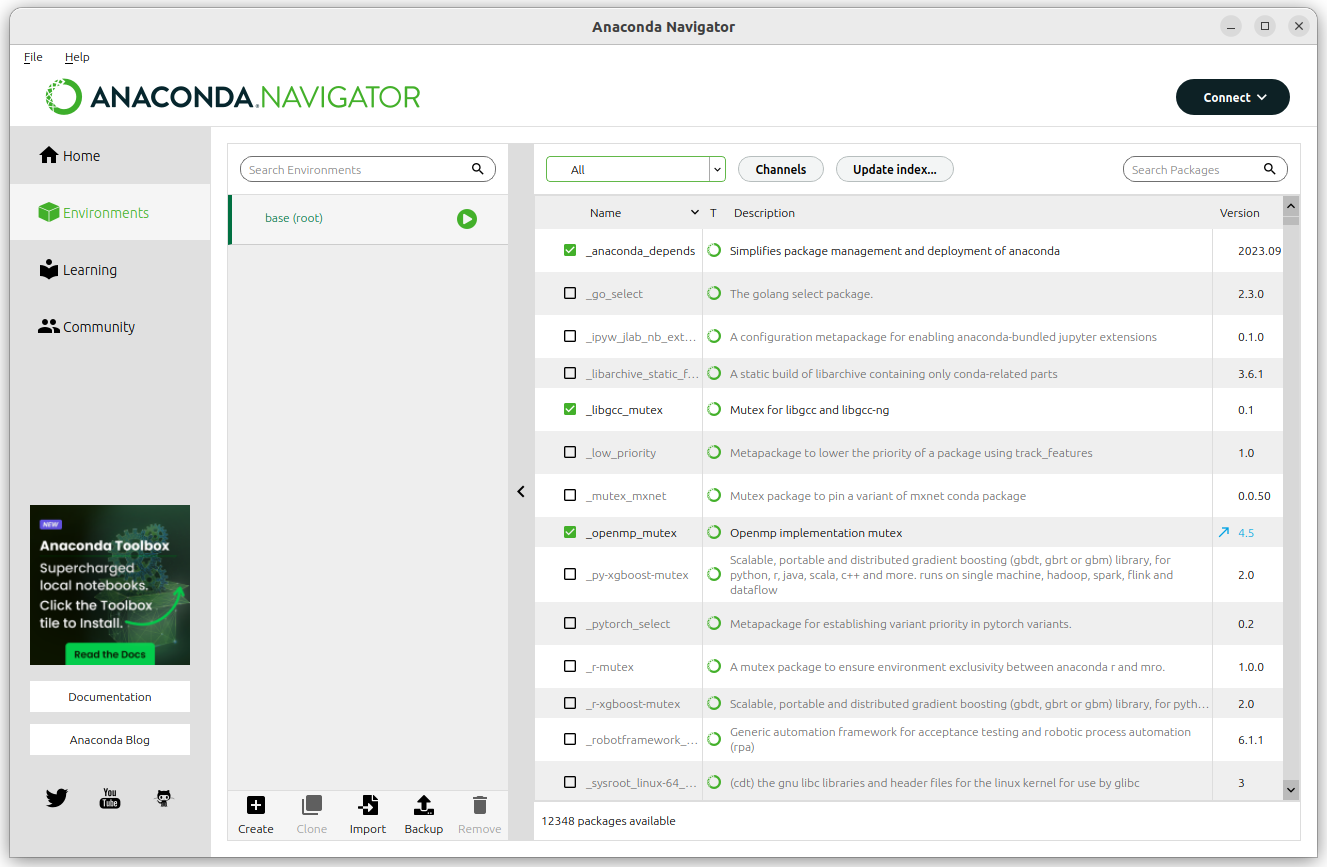
\includegraphics[width=0.8\textwidth]{notebook1.png}
    \caption{Ventana de Anaconda-Navigator, se ha señalado en rojo el botón Environments.}
    \label{fig:ntb1}
\end{figure}
\begin{paracol}{2}
 Hay instaladores de Anaconda disponibles para Windows, Linux y Mac. El proceso de instalación es en todos los casos bastante sencillo. La página web contiene además documentación en la que se explica detallademente el funcionamiento de Anaconda.

 Una vez instalado, Ananconda proporciona una aplicación (Navegador) desde la que manejarlo: \emph{anaconda-navigator}. Si ejecutamos Anaconda-Navigator, obtendremos una ventana como la que se muestra en la figura \ref{fig:anaconda}.

 El navegador de Anconda, muestra un conjunto de iconos. Cada uno de ellos corresponde a una aplicación distinta. Muchas de ellas están relacionadas con IDEs especialmente diseñados para usar Python, otras están relacionada con otros programas orientado al tratamiento de datos, las representaciones gráficas o la estadística. En algunos de los iconos aparece la palabra \emph{launch}. Indica que la aplicación se encuentra instalada en nuestro ordenador,. Si pulsamos con el ratón sobre el botón \emph{launch}, la aplicación se ejecuta. En otros casos, aparece la palabra \emph{install}. Se trata de aplicaciones que no están instaladas en nuestro ordenador, pero que pueden ser instaladas si pulsamos en botón \emph{install}. 

 En nuestro caso, vamos a emplear Spyder, que aparece entre las aplicaciones ya instaladas, y que aparece rodeada en la figura \ref{fig:anaconda} con un círculo rojo.

 Antes de entrar en la descripción de spyder, vamos a emplear Anaconda navigator para instalar un plug-in, que nos permitirá manejar desde spyder, otro de los entornos de programación de Python más empleados actualmente: \emph{Jupiter Notebook}. Jupiter Notebook, es en realidad un IDE para programar en Python independiente de Spyder. Es muy útil porque permite combinar código en python con texto y gráficos. Más adelante explicaremos como usarlo.

 \paragraph{Instalación de spyder-notebook.} para instalar el plug-in de Spyder que permite manejar notas de jupyter-notes, pulsamos en la ventana de Anaconda-Navigator el botón \emph{Environmets}, (enmarcado en rojo en la figura \ref{fig:anaconda2}). La ventana de Anaconda-Navigator nos muestra ahora los entornos de trabajo de Anaconda, (figura \ref{fig:ntb1}). Por defecto, estaremos en el entorno base (root). Este será además el único entorno disponible si acabamos de hacer una instalación de Anaconda nueva en el ordenador. Si seleccionamos \emph{All} en el menu desplegable situado en la parte superior izquierda del panel de la derecha,  obtenemos una relación de todos los paquetes disponibles en anaconda. Aquellos que ya están instalados aparecen marcados a la izquierda con un cuadro verde, mientras que para aquellos disponibles pero no instalados el cuadro aparece en blanco.

 En la parte superior derecha de éste panel hay un buscador. Si introducimos en el la palabra spyder, El panel nos mostrará los paquetes relacionados con Spyder (figura \ref{fig:ntb2}). Seleccionamos el paquete spyder notebook y en la parte inferior derecha del panel nos aparaceran dos nuevos botones. Si seleccionamos el botón \emph{apply}, Anaconda commenzará el proceso de instalación del paquete. Lo primero que hace es abrir un pop-up y comprobar las dependencias, una vez terminada la comprobación, pulsamos el botón apply del pop-up y dejamos que Anaconda instale spyder notebook.
 

 \switchcolumn
 \selectlanguage{english}
 Anaconda installers are available for Windows, Linux, and Mac. The installation process is straightforward. The Anaconda webpage offers complete information on installation and performance.

 Once installed, it supplies an application \emph{anaconda-navigator} to manage Anaconda. When we start Anaconda-Navigator, we get a window like that shown in figure \ref{fig:anaconda}.

 Anaconda-Navigator shows a set of icons. Anyone of them is intended to launch a different application. Many of them are IDEs specifically designed to use Python. Others relate to other programs devoted to data processing, graphics, or statistics. The work \emph{launch} is written in some of these icons. This means that the application has already been installed on our computer. Pressing the left-hand button of the mouse over the word \emph{launch} opens the application. In other cases, the word \emph{install} is Written over the icon. In these cases, the application is not installed on our computer, but we can install it by pressing the left-hand button of the mouse over the word \emph{install}.

 We are going to use Spyder, which has already been installed. In figure \ref{fig: anaconda}, the Spyder icon has been enclosed in a red circle.

 Before starting with a Spyder description, we will use Anaconda to install a plug-in, allowing us to use another of Phyton's most currently used IDEs: \emph{Jupyter Notes}. Jupyter Notes is an IDE for Python code development.  It is independent of Spyder. It is a handy tool because it allows us to combine Python code with graphics and text. We will describe Jupyter Notes later on.

 \paragraph{Spyder-notebook installation.} To install the plugin that allows using Jupyter Notes from Spyder, we press the mouse left button on the \emph{Environments} icon (framed in red in figure \ref{fig:anaconda2}). Then, the Anaconda-Navigator window shows us Anaconda work environments (figure \ref{fig:ntb1}). If we have just installed Anaconda, the only environment already available should be the base (root) environment. We will focus on the right-side panel. The upper left corner has a drop-down menu; we select the option \emph{all}. Then, the panel shows us all the software packages available in the Anaconda default channel. Those packages installed in the computer are ticked with a green square label before the package name; packages available but not installed are ticked with a white square.

 There is a browser located in the upper right corner of the panel. We will write the word \emph{spyder} of \emph{spyder notebook}. The panel now shows those software packages related to Spyder (figure \ref{fig:ntb2}). We select the package spyder notebook by clicking the white square before the package name. A new pair of push buttons appear on the panel's lower side. Clicking on \emph{apply} triggers the Spyder notebook installation process. First, Anaconda launches a pop-up window and checks Spyder Notebook software dependencies. The process may take some time, so be patient until it finishes the checking.  Once the checking process is over, we will press the \emph{apply} button on the pop-up window and let Anaconda install the software.
 
\end{paracol}
 
\begin{figure}
\centering
    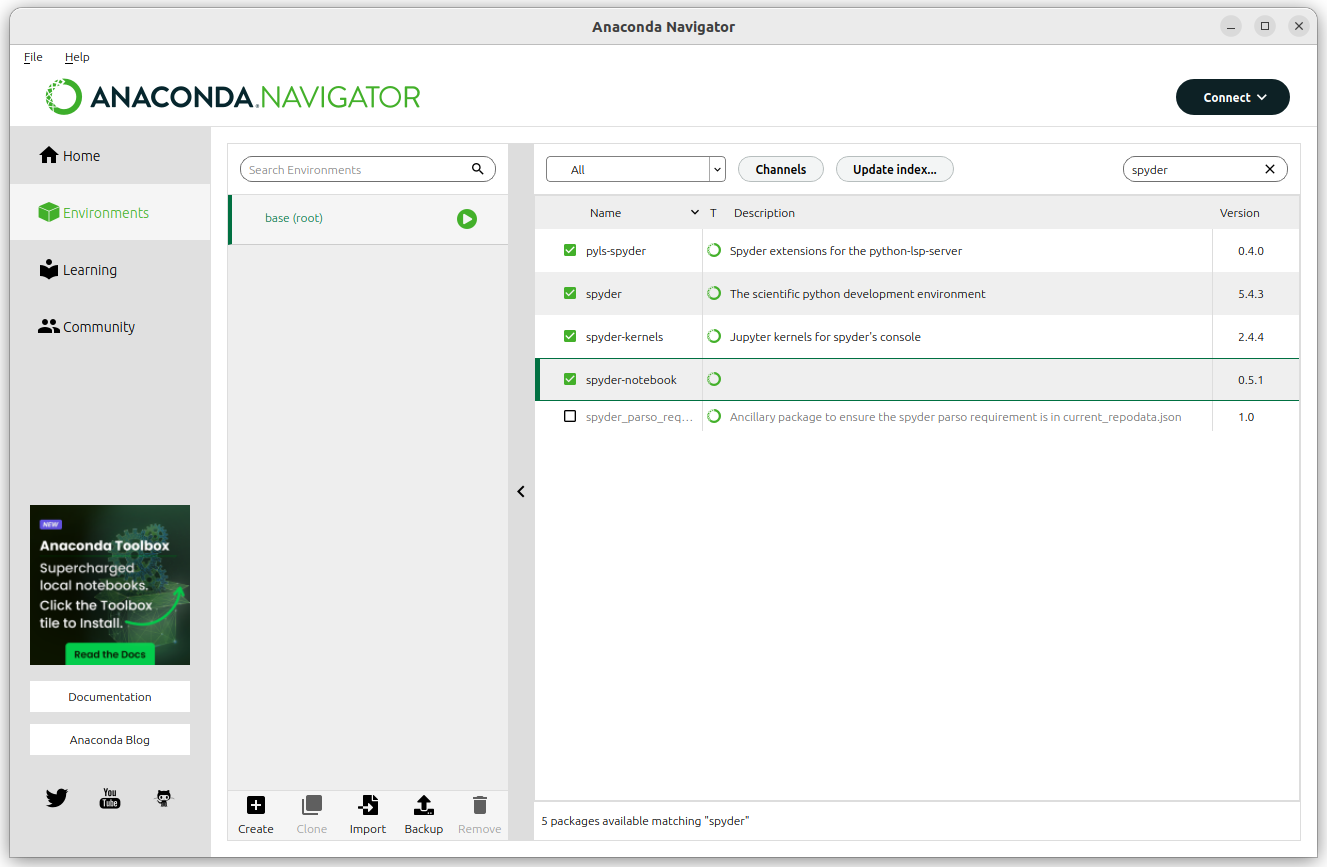
\includegraphics[width=0.8\textwidth]{notebook2.png}
    \bicaption{Ventana de Anaconda-Navigator, se ha señalado en rojo el botón Environments.}{Anaconda-Navgator window. The Environments button has been encircled in red}
    \label{fig:ntb2}

\end{figure}

\begin{figure}
\centering
    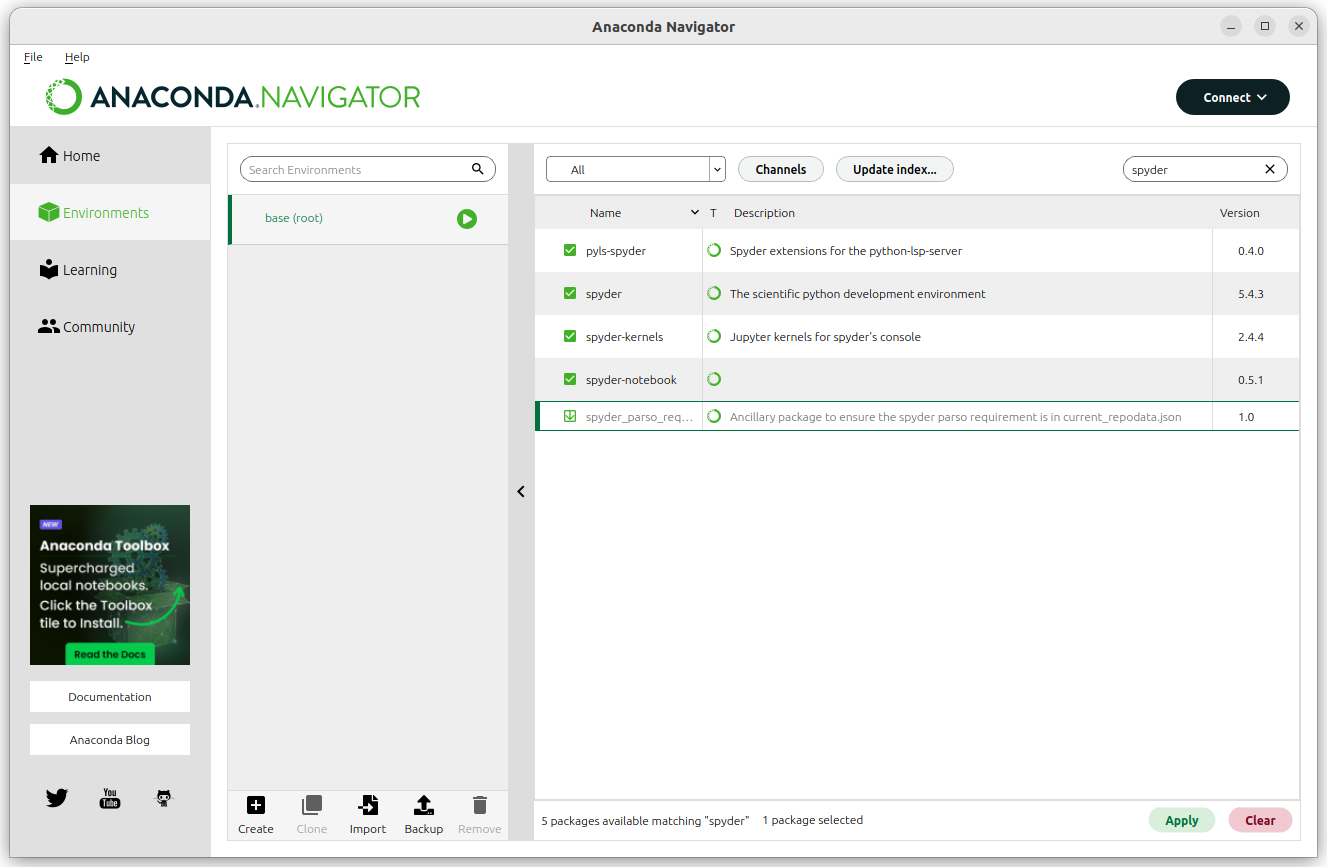
\includegraphics[width=0.8\textwidth]{notebook3.png}
    \bicaption{Ventana de Anaconda-Navigator, se ha señalado en rojo el botón Environments.}{Anaconda-Navgator window. The Environments button has been encircled in red}
    \label{fig:ntb3}
\end{figure} 

\begin{paracol}{2}
\subsection{Spyder}\index{Spyder}
Vamos a centrarnos en esta sección en describir Spyder. Como ya dijimos, Spyder es unn entorno de programación integrado, especialmente pensado para trabajar con Python en computación científica. Para lanzar el entorno basta con que pulsemos el botón \emph{launch} del icono de Spyder, en la ventana de Anaconda-navigator (figura: \ref{fig:anaconda}). Al hacerlo, se nos abrirá una nueva ventana como la que se muestra en la figura \ref{fig:ide}.

En la ventana de Spyder podemos distiguir tres paneles distintos\footnote{La configuración que Spyder que se describe  aquí, es la configuración por defecto. El usuario puede cambiarla a su gusto modificando los valores por defecto.}. Además, en la  parte superior de las ventamos tenemos una barra con menús deplegables y otra con botones. Vamos a describir brevemente algunas de las características principales del entorno a la vez que nos vamos introduciendo en las caracterís- ticas fundamentales de la programación en Py- thon. En cualquier caso, no vamos a dar una descripción exhaustiva. La mejor manera de aprender a manejar Spyder es usarlo y consultar la abundante documentación disponible.
\switchcolumn

\subsection{Spyder}\index[eng]{Spyder}
Let's focus on the Spyder description. As we said before, Spyder is an Integer Development Environment specially designed to use Python for scientific computing. To start Spyder, we push the \emph{launch} button on the Spyder Icon, located in the Anaconda-Navigator window (figure \ref{fig:anaconda}. Then, a new window opens, as shown in figure \ref{fig:ide}.

This (Spyder) window has three different panels\footnote{We describe here the default Spyder configuration. The user may change this default configuration according to their preferences.}. Besides, in the upper part of the window, there is a toolbar and a second bar that contains drop-down menus. We are going to give a brief description of the Spyder environment and, at the same time, some of Python programming's basic features. Anyway, we will not be exhaustive. An exhaustive description is far beyond the reach of these notes. The best way to learn to deal with Spyder is by using it. Moreover, there is a vast amount of available documentation.
\end{paracol}

\begin{paracol}{2}
\paragraph{El terminal mejorado de Python}\index{Ipython}
De los tres paneles mostrados en la figura \ref{fig:ide}, vamos a describir primero el situado abajo a la derecha. Este panel es un terminal, se conoce con el nombre de Ipython (Interactive python) y e incluye muchas mejoras sobre el terminal est estándar de python. Ipython nos muestra el símbolo \mintinline{python}{In [1]:}, que recibe el nombre de \emph{prompt}, y a continuacion una barra vertical $|$ parpadeante. El terminal permite al usuario interactuar directamente con Python; es decir, Python puede recibir instrucciones directamente a través del terminal, ejecutar las instrucciones, y devolver y/o guardar en memoria los resultados obtenidos.  Veamos un ejemplo. Si escribimos en el terminal:
\begin{minted}{python}
In [1]: 2+2
\end{minted}
y pulsamos la tecla \emph{intro}, Python calcula la suma pedida, muestra el resultado y nos desvuelve un nuevo prompt, esperando una nueva orden:
\begin{minted}{python}
Out[1]: 4
In [2]:
\end{minted}
Es interesante notar que el resultado nos lo ha mostrado empleando una marca de salida (\emph{eco}) \mintinline{python}{Out[1]:}. En programación, cuando una orden nos muestra por pantalla el resultado de la operción realizada, se dice que el ordenador ha hecho \emph{eco}. Como veremos más adelante esto no es lo más habitual, en la mayoría de los casos, el ordenador ejecuta la orden recibida y cuando termina nos devuelve el prompt \mintinline{python}{In [2]:} para indicarnos que ha terminado y está listo para recibir una nueva instrucción. De este modo, podemos emplear Python de modo análogo a como empleamos una calculadora. De hecho, la sintáxis es prácticamente la misma.
\switchcolumn
\paragraph{The Python's Enhance Terminal}
Returning to the three panels shown in figure \ref{fig:ide}, we will focus first on the left-down one. This panel is a Python console. The console displays a symbol \mintinline{python}{In [1]:} known as the \emph{prompt} followed by a flicking vertical bar. The console allows the user to interact with Python straight; i.e., Python can get direct instructions through the terminal, run the instructions, and show and/or save in memory the achieved results. Let's see an example. If we write in the console:
\begin{minted}{python}
In [1]: 2+2
\end{minted}
and press the intro key; Python calculates the sum, shows the result using an output (\emph{echo}) mark,  \mintinline{python}{Out [1]:}, gives back a new clean prompt, and stops waiting for a new command:
\begin{minted}{python}
Out[1]: 4
In [2]:
\end{minted}

In programming slang, it is usual to call the answer the computer shows on the screen an \emph{echo}. As we shall see later on, it is not usual for the computer to show us the result of the operations. Most of the time, it just executes the commands, and when it finishes, it shows us the prompt \mintinline{python}{In[2]:} again to tell us that it is ready for a new command. In this way, we can use Python as a calculator. The syntaxis is, indeed, quite similar.
\end{paracol}

\begin{figure}
	\centering
		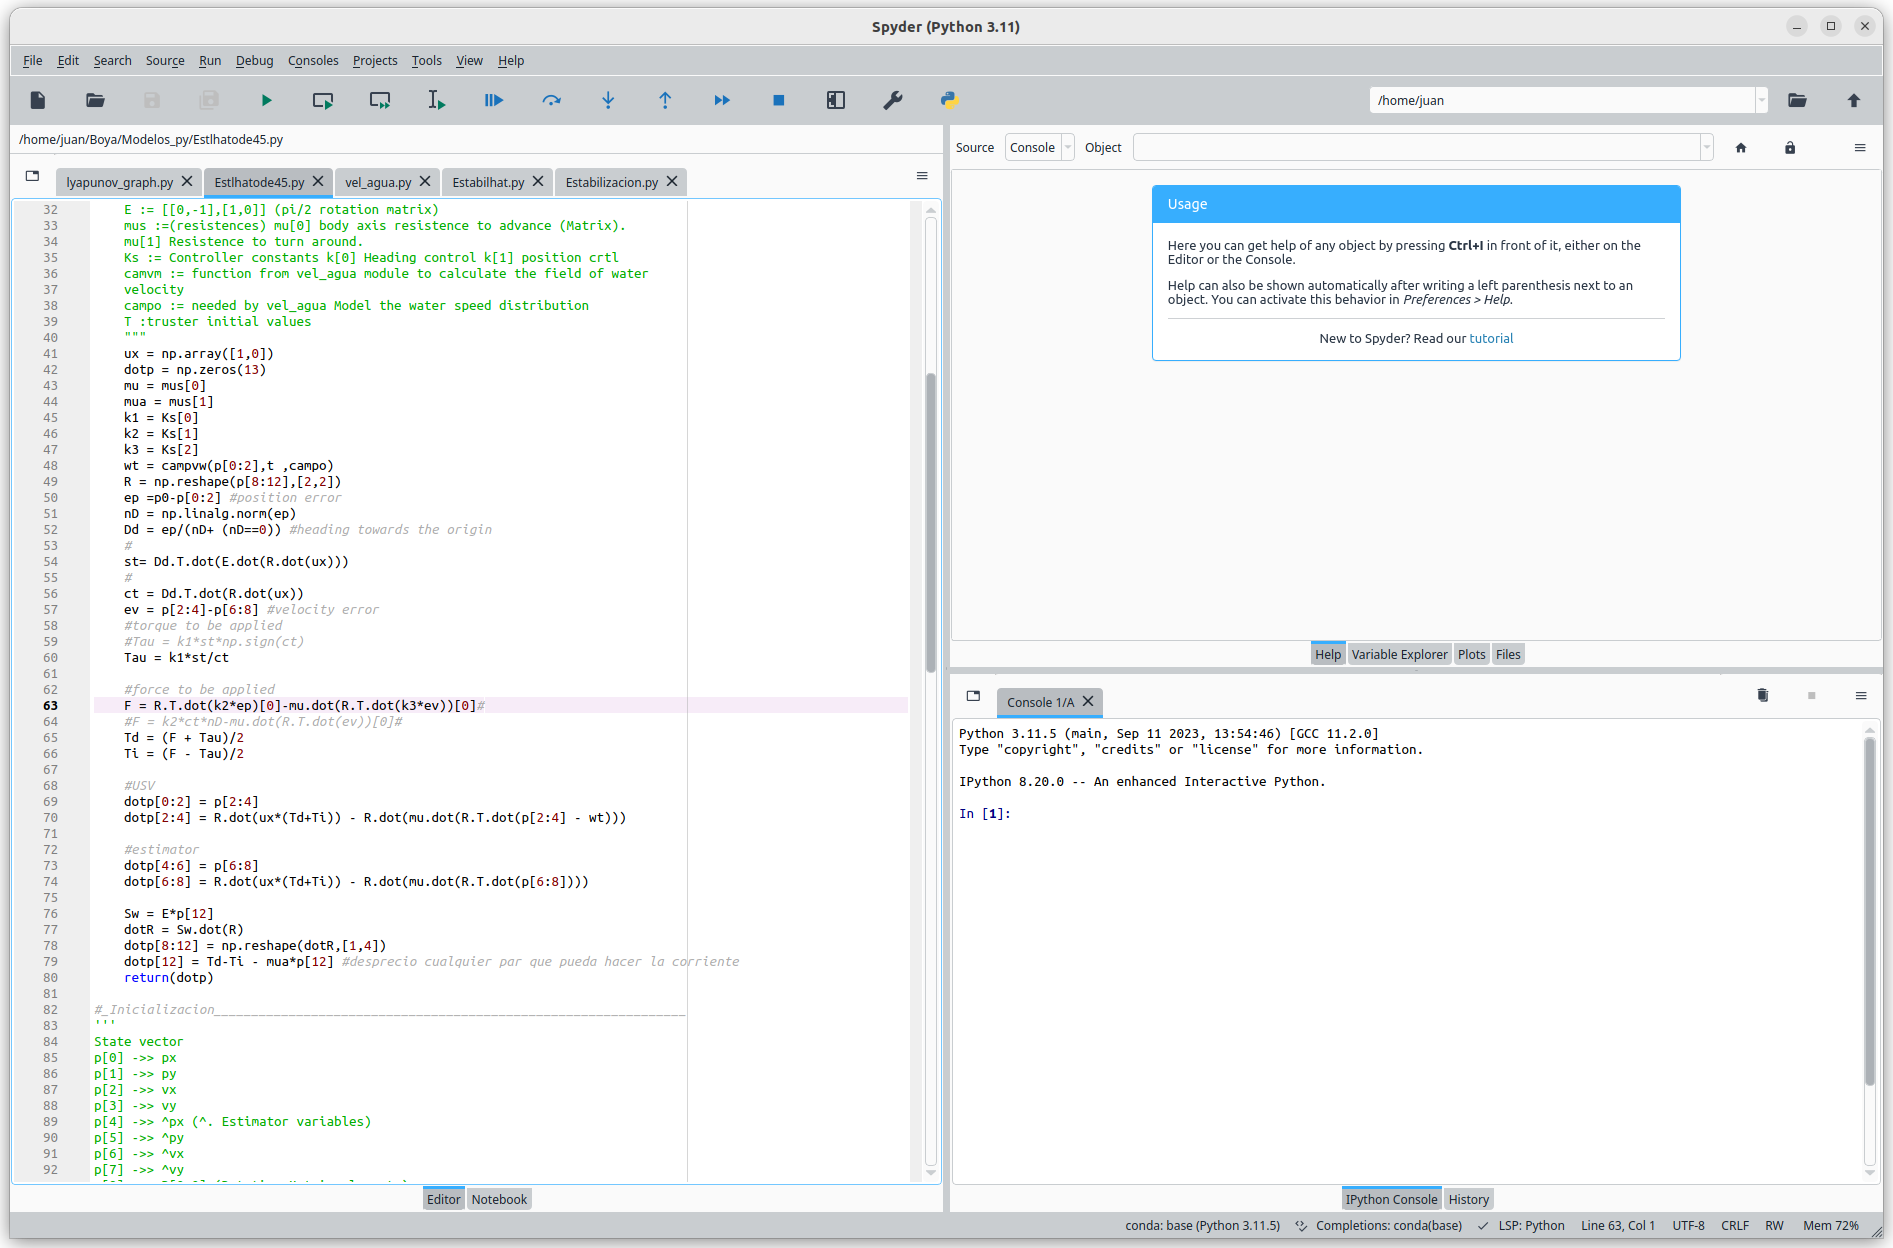
\includegraphics[width=14cm]{ide_n.png}
	\bicaption{Spyder: Entorno de desarrollo integrado para Python}{Spyder: An integer development environment for Python}
	\label{fig:ide}
\end{figure}

\begin{paracol}{2}
\subsection{Variables}\index{Variables}
El uso de Python como si fuera una calculadora no tiene demasiado interés. Una vez ejecutada la orden, tras pulsar la teccla \emph{intro} el ordenador no guarda ninguna información sobre la operación realizada. Si queremos realizar un cálculo complejo descomponiéndolo en más sencillas, deberemos anotar los resultados parciales y volver a copiarlos en el terminal si queremos emplearlos de nuevo. Por supuesto, hace ya mucho tiempo que alguien encontró una buena solución, para este y otros problemas similares: el uso de variables.

\switchcolumn
\subsection{Variables}\index[eng]{Variables}
Nevertheless, handling Python as a calculator is hardly ever enjoyable. Once a command has been executed after pressing the \emph{intro} key, the computer keeps no memory of the operation. If we wish to make a complex computation, splitting it into simpler operations, we should take note of the partial results and copy them again on the console to be used again. Of course, a long time ago, somebody found a good solution for this and other similar problems: using variables.

\switchcolumn
Podemos ver una variable como una región de la memoria del computador, donde un programa guarda una determina información: números, letras, etc. Una característica fundamental de una variable es su nombre, ya que permite identificarla. \index{Variable! nombre} Como nombre para una variable se puede escoger cualquier combinación de letras y números, empezando siempre con una letra, en el caso de Python\footnote{Como se verá más adelante, Python tiene un conjunto de nombres de instrucciones y comandos ya definidos. Se debe evitar emplear dichos nombres, ya que de hacerlo se puede perder acceso al comando de Python que representan}. Se puede además emplear el signo "\_". Python distingue entre mayúsculas y minúsculas, por lo que si elegimos como nombres de variable Pino, PINO y PiNo, Matlab las considerará como variables distintas. 

\switchcolumn
We can consider a variable as a computer memory region where a program has allocated specific information: numbers, characters, etc. A variable fundamental characteristic is its name because it permits one to identify it univocally. \index[eng]{Variable! name}. We can take as a variable name whatever combination of lowercase and uppercase letters and numbers, provided that the first character is always a letter. When using Python\footnote{As we shall see later on, Python has a set of command names and keywords already defined. We should avoid using these names or keywords as names for our variables. Otherwise, we could lose access to the corresponding Python command or keyword.}, We may also use the symbol ''\_". For Python, uppercase and lowercase letters are different symbols. Thus, if we choose variable names, such as Oack, OACK, and OaCk, they represent different variables for phyton.

\switchcolumn
El método más elemental de crear o emplear una variable es asignarle la información para la que se creó. Para hacerlo, se emplea el símbolo de asignación \index{"= Símbolo de asignación} \index{Símbolo de asignación}, que coincide con el signo $=$ empleado en matemáticas. Como veremos más adelante la asignación en programación y la igualdad en matemáticas no representan exáctamente lo mismo. La manera de asignar directamente información a una variable es escribir el nombre de la variable, a continuación  el signo de asignación y, por último, la información asignada, \mintinline{python}{variable_1 = 18}. Si escribimos dicha expresión en la terminal de Python y pulsamos la tecla \emph{intro}:
\begin{minted}{python}
In [2]: variable_1 = 18
In [3]:
\end{minted}
En este caso, Python no hace eco, no nos muestra por pantalla ningún resultado. Sin embargo, la variable ha quedado guardada en la memoria del ordenador. Podemos pedirle a Python que nos la muestre, 
\begin{minted}{python}
In [3]: variable_1
Out[3]: 18

In [4]: print(variable_1)
18

In [5]: 
\end{minted}
En el primer caso, hemos escrito directamente el nombre de la variable en e prompt de IPython. En el segundo, hemos hecho uso de una función de Python \mintinline{python}{print()}. Mas adelante veremos con detalle las funciones en Python. Por el momento, es suficiente con decir que una función es un objeto de programación que toma una variable de entrada y opera sobre dicha variable y nos devuelve un resultado. La  función \mintinline{python}{print()} toma como variable de entrada, una variable cualquiera y nos imprime en el terminal de Ipython su contenido.

Podemas asignar también a una variable el resultado de una operación aritmética,
\mint{python}{In [5]: variable_2 = 2 * 5}

Para saber qué variables tiene guardadas el ordenador en memoria, podemos emplear algunos de los comandos especiales de la consola de Ipython,

\switchcolumn
The most straightforward method to create or use a variable is to assign the information we want to contain. To do this, we use the assignment symbol \index[eng]{= assignment symbol} \index[eng]{Asignment Symbol}, which coincides with the mathematical symbol $=$. As will be seen later, programming assignment and mathematical equality are not the same concept. To assign some piece of information to a variable, we write the variable name, then the assignment symbol, and, eventually, the assigned information \mintinline{python}{variable_1 = 18}. If we write this expression on the console and press the \emph{intro} key, we get:
\begin{minted}{python}
In [2]: variable_1 = 18
In [3]:
\end{minted}
In this case, the computer doesn't echo the result. Anyway,  the variable has been saved in the computer's memory. We may ask Python to show it,

\begin{minted}{python}
In [3]: variable_1
Out[3]: 18

In [4]: print(variable_1)
18

In [5]: 
\end{minted}
In the first case, we have written the name of our variable straightforwardly after the Ipython prompt. In the second case,  we use the Python function \mintinline{python}{print()}. Later on, we will see the concept of function in Python in more detail. Meanwhile, it is enough to say that a function is a programming object that takes an input variable, operates it and returns a result. In our case, the function \mintinline{python}{print()} takes a variable whatsoever and prints in the Ipython console the content of the variable.

We can also assign to a variable the result of an arithmetic operation,
\mint{python}{In [5]: variable_2 = 2 * 5}

To know which variables are saved in the computer memory, we can use some special Ipython console commands:
\end{paracol}

\begin{center}
\begin{minipage}{0.4\textwidth}
\begin{minted}{python}
In [5]: %whos
Variable          Type    Data/Info
-----------------------------------
variable_1        int     18
variable_2        int     10



In [6]: %who
variable_1	 variable_2    
\end{minted}
\end{minipage}
\end{center}

\begin{paracol}{2}
 En el primer caso, hemos empleado el comando de Ipython \mintinline{python}{whos}. Delante del comando hemos puesto el carácter \%, que sirve para indicar al ordonedar que se trata de un comando de de la Consola y no de Python. El ordenador nos muestra todas las variables que hemos definido, el tipo de variable y el dato que contienen. En el segundo caso hemos empleado el comando \mintinline{python}{who}, que nos da simplemente una lista de las variables contenidas en memoria. 

 \switchcolumn
 In the first case, we used the Ipyhon command \mintinline{python}{whos}. Notice that we have written the symbol \% just before the command. This tells the computer we are introducing a console (Ipython) command, not an ordinary Python command. The computer displays the variables we have defined until this point, the variable Type, and the data contained. In the second case, we have used the command \mintinline{python}{who}, which shows us the bare list of the variables saved in the computer memory.
 \switchcolumn Acabamos de mencionar, el concepto de tipo de una variable.\index{Variable! tipo} En algunos lenguaje, es preciso indicar al ordenador qué tipo de información se guardará en una determinada variable, antes de poder emplearlas. Esto permite manejar la memoria del computador de una manera más eficiente, asignando zonas adecuadas a cada variable, en función del tamaño de la información que guardarán. A este proceso, se le conoce con el nombre de \emph{declaración} de variables. En Python no es necesario declarar las variables antes de emplearlas. El tipo de dato se asigna directamente cuando la variable se crea, de acuerdo con la información asignada. Para saber el tipo de dato que contiene una variable se le aplica la función \mintinline{python}{type()} Vamos a ver los tipos de datos estándar o \emph{built-in} de Python.

\paragraph{Numeric.} Se trata de datos que corresponden a valores o cantidades numéricas. Dentro de los datos numéricos, Python define tres tipos distintos:

\emph{Integer.} Permite definir números enteros positivos y negativos. El tipo se representa mediante la abreviatura \emph{int}. Una caraterística específica de los enteros en Python es que no tienen limitación de tamaño.
\switchcolumn
We just mentioned the \emph{type} of a variable.\index[eng]{Variable! Type} In some programming languages, it is necessary to explicitly say the kind of information a variable will store before using it. The sort of information stored defines the type of the variable. This helps to manage the computer memory more efficiently, assigning memory zones according to the variable size. This process is known as variable \emph{declaration}. In Python, it is not necessary to declare variables. Python sets the type to a variable when it is created. To Know the data type of a variable, we use the function \mintinline{python}{type()}. Let's see standard or built-in types in Python.

\paragraph{Numeric.} Data which represent numerical quantities. Inside the numeric data, Python defines three different types:

\emph{Integer.} It allows for representing whole numbers, positives, and negatives. The type is represented by the abbreviation \emph{int}. A specific feature of integers in Python is that they have no size limitation.
\end{paracol}

\begin{figure}[thp]
\centering
\begin{minipage}{0.2\textwidth}
\begin{minted}{python}
In [92]: a = 35
In [93]: type(a)
Out[93]: int
\end{minted}
\end{minipage}
\end{figure}
\begin{paracol}{2}   
\emph{Float.} Permite definir números en coma flotante, es decir, una representación aproximada de un número real. (ver el capítulo \ref{chp:arit}). Se pueden introducir separando la parte entera de la decimal mediante un punto y tambien en notación científica. El tipo se representa mediante la abreviatura \emph{float}.

Es interesante notar que, \mintinline{python}{a = 3} Creará una variable entera mientras que \mintinline{python}{a=3.} creará una variable real.
\switchcolumn
\emph{Float.} Floating point numbers, i.e., approximated representations of real numbers. (See chapter \ref{chp:arit}). We use a point to split the integer and decimal parts of the number. It is also possible to write a floating point number using scientific notation. This type is represented by the word \emph{float}.

Notice that \mintinline{python}{a = 3} creates an integer variable, but \mintinline{python}{a=3.} creates a real variable. 
\end{paracol}

\begin{center}
\begin{minipage}{0.2\textwidth}
\begin{minted}{python}
In [95]: b = -3.5
In [96]: type(b)
In [94]: type(a)
Out[94]: intOut[96]: float
In [98]: c = 3e -4
In [99]: type(c)
Out[99]: float
\end{minted}
\end{minipage}
\end{center}


\begin{paracol}{2}        
\emph{Complex.} Por último, es posible tambier manejar en Python números complejos. Para ello hay que definirlos como la suma de su parte real más su parte imaginaria que va siempre seguida del simbolo \mintinline{python}{j}. Aunque introduzcamos las partes reales e imaginarias de un número complejo como enteros, Python siempre los considera números en coma flotante.
\switchcolumn Finally, it is possible in Python to deal with complex numbers. To define them, we write the real part of the number, the addition symbol, and the imaginary part, followed by the symbol \mintinline{python}{j}. Notice that Python considers a complex number's real and imaginary parts as floating point numbers even if you write them as integers.  
\end{paracol}

\begin{center}
\begin{minipage}{0.2\textwidth}
\begin{minted}{python}
In [100]: d = 2+3j
In [101]: type(d)
Out[101]: complex
In [102]: d.real #parte real
#del número d
Out[102]: 2.0
In [103]: d.imag #parte imagi-
#naria del número d
\end{minted}
\end{minipage}
\end{center}


\begin{figure}
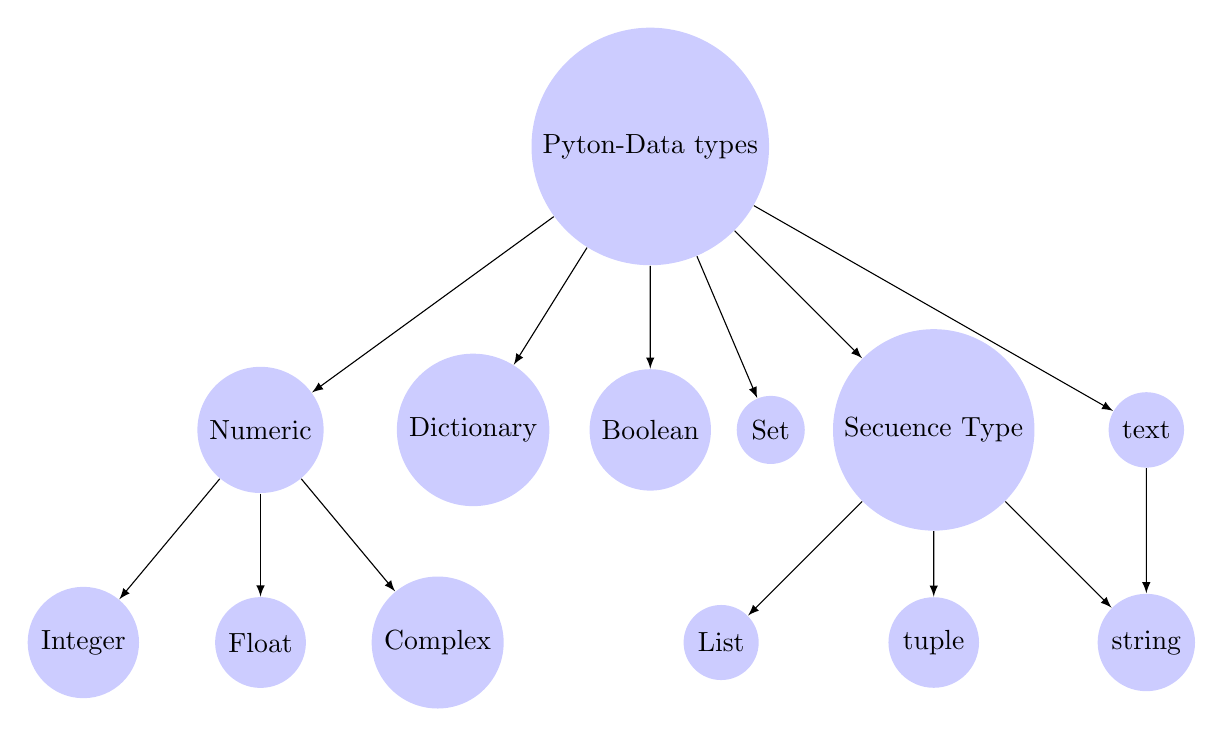
\begin{tikzpicture}
  [scale=.9,auto=center,every node/.style={circle,fill=blue!20}]     
  \node (a1) at (8,5) {Pyton-Data types};  
  \node (a2) at (2.5,1)  {Numeric}; 
  \node (a3) at (5.5,1) {Dictionary};  
  \node (a4) at (8,1)  {Boolean};  
  \node (a5) at (9.7,1)  {Set};  
  \node (a6) at (12,1)  {Secuence Type};
  \node (a13) at (15,1) {text};
  \node (a7) at (0,-2)  {Integer};
  \node (a8) at (2.5,-2)  {Float};
  \node (a9) at (5,-2) {Complex};
  \node (a10) at (9,-2) {List};
  \node (a11) at (12,-2) {tuple};
  \node (a12) at (15,-2) {string};
  
  \draw [-latex](a1) -- (a2);  
  \draw [-latex](a1) -- (a3);  
  \draw [-latex](a1) -- (a4);  
  \draw [-latex](a1) -- (a5);  
  \draw [-latex](a1) -- (a6);  
  \draw [-latex](a2) -- (a7);  
  \draw [-latex](a2) -- (a8);
  \draw [-latex](a2) -- (a9);
  \draw [-latex](a6) -- (a10);
  \draw [-latex](a6) -- (a11);
  \draw [-latex](a6) -- (a12);
  \draw [-latex](a13) -- (a12);
  \draw [-latex](a1) -- (a13);
  \end{tikzpicture}
  \bicaption{Tipos de datos en Python.}{Data types in Python}
\end{figure}

\begin{paracol}{2}
\paragraph{Boolean.} Como veremos más adelante, es muy frecuente en programación necesitar saber si una condición se cumple (es verdadera) o no (es falsa) esto lleva a que en muchos lenguajes de programación, existe un tipo de variable que solo toma dos valores: \mintinline{python}{True} (verdadero)  o \mintinline{python}{False} (falso).

\switchcolumn
As we will see later, it is widespread in programming to check if a condition fulfils (it is true) or not (it is false). This leads to many programming languages to define a type of variable that can take just two possible values:  \mintinline{python}{True} or \mintinline{python}{False}. 
\end{paracol}
\begin{center}
    \begin{minipage}{0.2\textwidth}
\begin{minted}{python}
In [1]: D = True
In [2]: type(D)
Out[2]: bool
\end{minted}
\end{minipage}\end{center}

\begin{paracol}{2}
\paragraph{Sequence Type}
    Todos los tipos incluidos en Sequence Type, así como los tipos diccionary y set, son en realidad estructuras de datos. Podemos verlos como contenedores, que nos permiten almacenar y manipular varios (muchos) datos distintos empleando una sola variable.
         
         \emph{String.} Es el formato propio para crear variables que contengan texto. Se construyen a partir de caracteres UNICODE, encerrados entre comillas,

\switchcolumn
\paragraph{Sequence Type} Every kind of variable included in Sequence Type, and also the types dictionary and set, are Data structures. We can see them as containers that allow us to deal with several (many) data using a single variable.

\emph{String} This is the proper type to generate variables that contain text. They are built using UNICODE characters enclosed in brackets.

\end{paracol}
\begin{center}
\begin{minipage}{0.2\textwidth}
\begin{minted}{python}
In [3]: tex1 = 'a'
In [4]: type(tex1)
Out[4]: str
In [5]  tex2 ='perro'
In [6]: type(tex2)
Out[6]: str
\end{minted}
\end{minipage}
\end{center}

\begin{paracol}{2}
Una propiedad común a todos los tipos sequence es que son indexables.\index{indexación} La indexación es una propiedad muy importante que vamos a emplear habitualmente en programación. La variable \mintinline{python}{tex2} del ejemplo anterior contiene en realidad una cadena de caracteres; las letras que componen la palabra \emph{perro}. Python nos permite extraer individualmente dichos caracteres empleando para ello un índice correpondiente a la posición que ocupan en la cadena. Para ello, escribimos el nombre de la variable seguido del índice encerrado entre corchetes. Hay que tener en encuenta que al primer elemento de una secuencia le corresponde el índice cero.

\switchcolumn
A common property of all types belonging to Sequence Type is that they are indexable. \index[eng]{indexation}. The indexation is a fundamental property that we frequently use in programming. The variable \mintinline{python}{tex2} in the previous example is an array of characters, the letters that compound the work \emph{perro} (Dog in Spanish HA,  HA). Using an index, Python, allows us to extract such characters individually. The index represents the position the character we want to extract takes in the word. To extract a character from a variable of type String, we write the variable's name followed by the character's index enclosed in square brackets. It is important to note that Python begins to count the elements of a sequence in zero.  
\end{paracol}

\begin{center}
    \begin{minipage}{0.3\textwidth}
\begin{minted}{python}
In [7]: letra_1 = tex[0]
In [8]: print(letra_1)
p
In [9]: letra_4 = tex[3]
In [10]: print(letra_4)
r
\end{minted}
\end{minipage}
\end{center}
\begin{paracol}{2}
Python permite también indexar una secuencia, empezando por el final. En esta caso, al último elemento le corresponde el índice  \mintinline{python}{-1}, al penúltimo \mintinline{python}{-2}, etc,
\switchcolumn
Python also permits indexing a sequence beginning by the end. In this case, the sequence's last element takes the index -1, the next-to-last takes -2, and so on. 
\end{paracol}

\begin{center}
    \begin{minipage}{0.3\textwidth}
\begin{minted}{python}
In [40]: tex[-1]
Out[40]: 'o'
In [41]: tex[-3]
Out[41]: 'r'
\end{minted}
\end{minipage}
\end{center}

\begin{paracol}{2}
\emph{Listas.} Las listas en python son colecciones ordenadas de datos. Los elementos de una lista pueden ser datos de cualquier tipo y no tienen por qué ser homogeneos, Para crear una lista basta escribir los elementos que la componen entre corchetes y separados por comas,
\switchcolumn
Lists are ordered collections of data. The elements of a list can be data of whatever type, and they do not need to be homogeneous. To create a list, write the elements that built it up, enclosed in square brackets and separated by commas.  
\end{paracol}

\begin{center}
    \begin{minipage}{0.4\textwidth}
\begin{minted}{python}
In [11]: L = ['carta', 23, 2.5, 1-2j]
In [12]: L
Out[12]: ['carta', 23, 2.5, (1-2j)]
In [13]: type(L)
Out[13]: list
\end{minted}
\end{minipage}
\end{center}

\begin{paracol}{2}
Hemos construido una lista en la que el primer elemento es una cadena, el segundo un entero, el tercero un float y el cuarto un número complejo. Debido a su versatilidad, las listas son un tipo de variable muy empleado en Python. Pdemos copiar elementos de una lista a otra variable empleando índices, y tambien podemos asignar a un elemento de una lista un valor nuevo, por supuesto, perderemos el valor antiguo,
\switchcolumn
We had built a list in which the first element is a string, the second an integer, the third a real --float type-- number, and the fourth is a complex number. Due to their versatility, the Lists are a very useful type in Python. We can copy elements of a list in another variable using indexes and assign a new value to an element of a list. Of course, in this case, we will lose the old value. 
\end{paracol}

\begin{center}
    \begin{minipage}{0.2\textwidth}
\begin{minted}{python}
In [14]: L3 = L[3]
In [15] print(L3)
(1-2j)
In [16]: L[2] = 0.
In [17]:print(L)
['carta',0.0,2.5,(1-2j)]
\end{minted}        
    \end{minipage}
\end{center}

\begin{paracol}{2}
Dado que una lista no es más que una colección ordenada de variables, podemos anidar listas dentro de listas,
\switchcolumn
As far as a list is nothing more than an ordered collection of variables, we can nest a list inside another list,
\end{paracol}

\begin{center}
\begin{minipage}{0.3\textwidth}
\begin{minted}{python}
In [14]: LL = [1, 'p,,L,-0.7]
In [15]: print(LL)
[1, 'p', ['carta', 23, 2.5, (1-2j)], -0.7]
\end{minted}
\end{minipage}
\end{center}

\begin{paracol}{2}
Hemos incluido la lista \mintinline{python}{L} como el tercer elemento de la nueva lista \mintinline{python}{LL}. Podemos extraer un elemento de la lista interior, empleando dos índices; el primero para referirnos a la posición de la lista \mintinline{python}{L} dentro de la lista  \mintinline{python}{LL}, y el segundo para indicar la posición del elemento deseado dentro de la lista \mintinline{python}{L}. Así por ejemplo, si queremos obtener la palabra 'carta'`,
\switchcolumn
We have included the list \mintinline{python}{L} as the third element of a new list \mintinline{python}{LL}. We can extract an element from the inner list using two indexes. The first one indicates the position of the list \mintinline{python}{L} inside the list \mintinline{python}{LL}, and the second one indicates the position of the wanted element inside the list \mintinline{python}{L}. For instance, if we want to get the word 'carta',
\end{paracol}

\begin{center}
\begin{minipage}{0.3\textwidth}
 \begin{minted}{python}
 In [16]: ctr = LL[2][0]
 In [17]: print(ctr)
 carta
\end{minted}
\end{minipage}
\end{center}
\begin{paracol}{2}
Podemos cambiar datos de una lista, usando el simbolo de asignación,
\switchcolumn
We can change list data using the assignation symbol,
\end{paracol}
\begin{center}
\begin{minipage}{0.5\textwidth}
\begin{minted}{python}
In [18]: LL[3] = 'J'
In [19]: print(LL)
[1, 'p', ['carta', 23, 2.5, (1-2j)], 'J']
\end{minted}
\end{minipage}
\end{center}

\begin{table}
\centering
    \begin{tabular}{l l l}
    append() & añade un elemento al final de la lista & \mintinline{python}{L.append(-3)}\\
    & adds a element to the end of a list & \\
    \hline
    copy() & Crea una copia de la lista & \mintinline{python}{L2 = L.copy()}\\
    & Returns a copy of a list & \\
    \hline
     clear() & Borra todos los elementos de una lista & \mintinline{python}{L.clear}\\
     &clears all elements from a list&\\
     \hline
     count()& Cuenta el número de elementos de una lista & \mintinline{python}{L.count()}\\
     &Counts the elements of a list&\\
     \hline
     insert() & Inserta un nuevo elemento en una posición específica & \mintinline{python}{L.insert(i,-4}\\
     &Inserts an element at a specific position in a list &\\
     \hline
     pop() & Extrae el ultimo elemento de una lista.  &\mintinline{python}{a =L.pop()}\\
     & Si se añade un índide extrae el elemnto indicado &\mintinline{python}{a=L.pop(i)}\\
     & extract the last element of a list. &\\
     &Addind and index, extract the specific element& \\
     \hline
    \end{tabular}
    \bicaption{Algunos métodos de las Listas en Python}{Some methods of Python's List}
    \label{Tb:listas}
\end{table}

\begin{paracol}{2}
Una caracterítica importante de las listas, son sus métodos. Los métodos son funciones especiales que nos permiten manipular las listas de una manera directa. La tabla \ref{Tb:listas} muestra algunos de los más usuales. La forma de emplearlos es escribir el nombre de la lista, seguido de un punto el nombre del método y, entre paréntesis los parámetros que toma. Si el método no toma ningún parámetro se deja el paréntesis vacío, pero nunca se omite. Veamos algunos ejemplos:
\switchcolumn
An essential feature of Lists is their methods. The methods are special functions that allow us to manipulate the lists in a straight way. Table \ref{Tb:listas} shows some of the most used list methods. To use a method, we write the list name followed by a point and name of the method and, enclosed in brackets, the parameters the method takes. If the method doesn't use parameters, we write an empty bracket after the method name but never leave it off. Let's see some examples:
\end{paracol}

\begin{center}
    \begin{minipage}{0.5\textwidth}
\begin{minted}{python}
In [12]: L = [1, 'a',-0.5,'en',2.5,'a']
In [13]: print(L)
[1, 'a', -0.5, 'en', 2.5, 'a']
In [14]: L.append(-2)
In [15]: print(L)
[1, 'a', -0.5, 'en', 2.5, 'a', -2]
In [16]: L.pop()
Out[16]: -2
In [17]: print(L)
[1, 'a', -0.5, 'en', 2.5, 'a']
In [18]: L.insert(3,'insrt')
In [19]: print(L)
[1, 'a', -0.5, 'insrt', 'en', 2.5, 'a']
In [20]: L.pop(3)
Out[20]: 'insrt'
In [21]: print(L)
[1, 'a', -0.5, 'en', 2.5, 'a']
In [22]: L.count('a')
Out[22]: 2
In [23]: L.count('s')
Out[23]: 0
\end{minted}
    \end{minipage}
\end{center}

\begin{paracol}{2}

\emph{Tuplas} Las tuplas, son similares a las listas. La principal diferencia es que son inmutable. es decir, una vez que se han creado no se puede modificar el valors de los elementos que contiene. Para crearlas se encierran los elementos que constituyen la tupla entre paréntesis y separados con comas. En el ejemplo que sigue se observa como al intentar modificar un elemento de una tupla una vez creada, Python nos desvuelve un aviso de error.
\switchcolumn

\emph{tuples} Tuples are similar to List. The main difference between them is that Tuples are immutable, i.e., once created, the elements of a Tuple cannot be modified. To build a Tuple, we enclose their elements into brackets, separated by commas. The following example shows how Python throws an error message when we try to modify a Tupla element once it has been built.
\end{paracol}

\begin{center}
\begin{minipage}{0.4\textwidth}
\begin{minted}{python}
In [41]: T = (0,'int',2.4,[1,4,3.5])
In [42]: T
Out[42]: (0, 'int', 2.4, [1, 4, 3.5])
In [43]: T = (0,'int',2.4,[1,4,3.5])
In [44]: print(T)
(0, 'int', 2.4, [1, 4, 3.5])
In [45]: type(T)
Out[45]: tuple
In [46]: T[3]
Out[46]: [1, 4, 3.5]
In [47]: T[4] = 12
Traceback (most recent call last):
  Cell In[47], line 1
    T[4] = 12
TypeError: 'tuple' object does not support item assignment

\end{minted}
\end{minipage}
\end{center}

\begin{paracol}{2}
\paragraph{Dictionary.} Los diccionarios son estructuras en las que los datos aparecen asociados a claves. La forma más sencilla de crearlos es mediante pares clave:dato separados por comas y encerrados entre llaves. El símbolo ':' asocia cada elemento con su clave. Un diccionario puede contener dentro cualquier tipo de variable, incluidas listas u otros diccionarios. Para acceder a un elemento guardado en un diccionario se escribe el nombre del dicionario seguido de la clave del elemento deseado escrita entre corchetes.

\switchcolumn
A dictionary is a structure in which data are associated with keys. The simplest way to create them is by using a pair key: data separated by commas and enclosed in curly braces. The symbol ':' associates each element with its key. A dictionary can contain whatever type of variable, including lists and other dictionaries. To get access to data stored in a dictionary, we write the name of the dictionary followed by the key of the element we want to access, enclosed in square brackets.
\end{paracol}


\begin{minted}{python}
In [63]: D = {'nombre':'Pepe','día':27, 'mes':'Febrero', 'datos':[1,3.5,6,0.0]}
In [64]: D
Out[64]: {'nombre': 'Pepe', 'día': 27, 'mes': 'Febrero', 'datos': [1, 3.5, 6, 0.0]}
In [65]: type(D)
Out[65]: dict
\end{minted}        


\begin{paracol}{2}
Para añadir nuevos elementos a un diccionario, se emplea el nombre del diccionario seguido de la clave que tendrá el elemento, escrita entre corchetes y se usa el simbolo de asignación para añadir el valor del elemento. Al igual que sucedía en el caso de las listas, es posibles anidar diccionarios dentro de otros diccinarios. Para acceder al diccionario interno, empleamos su clave. Para acceder a un elemento del diccionario interno empleamos la clave del diccionario interno seguida de la clave del elemento. Para borrar un elemento de un diccionario empleamos la orden de python \mintinline{python}{del()}. Igual que las listas, los diccionarios cuentan con un buen número de metodos propios. Los interasados pueden consultarlos en las páginas de referencia de Python.
\switchcolumn
To add new elements, we write the name of the dictionary followed by the key we want to assign to the element, enclosed in square brackets, and we use the assignation symbol to add the element value. As in the case of lists, it is possible to nest one dictionary into another. To access the inner dictionary, we use its key. To access data inside the inner dictionary, we use the inner dictionary key followed by the data key. (see In[78]: in the example below). To eliminate an element from a dictionary, we use the Python command \mintinline{python}{del()}. Similar to the Lists, there are quite a few dictionary methods. Readers interested should be addressed to Python reference pages.
\end{paracol}

\begin{minted}{python}

In [75]: D['nuevo'] = {'calle':'Atocha','num.':18,'Piso':'3D'}

In [76]: D
Out[76]: 
{'nombre': 'Pepe',
 'día': 12,
 'mes': 'Febrero',
 'datos': [1, 3.5, 6, 0.0],
 'nuevo': {'calle': 'Atocha', 'num.': 18, 'Piso': '3D'}}
In [77]: D['día']
Out[77]: 12
In [78]: D['nuevo']['num.']
Out[78]: 18
In [81]: del(D['día'])
In [82]: D
Out[82]: 
{'nombre': 'Pepe',
 'mes': 'Febrero',
 'datos': [1, 3.5, 6, 0.0],
 'nuevo': {'calle': 'Atocha', 'num.': 18, 'Piso': '3D'}}
\end{minted}


\begin{paracol}{2}
\paragraph{Set.} Los conjuntos son colecciones datos no repetidos e inmutables. Para crear un conjunto en Python se escriben sus elementos separados por comas y encerrados entre llaves. Si hay elementos repetidos en la definicion, el conjunto creado solo los contendrá una vez. No vamos a verlos en más detalle.
\switchcolumn
\paragraph{Set.} Sets are inmutable non-repited data collections. To make a set in Python we writen its elements separated by commas and enclosed in curly braces. If there are repited elements in its definition, the set created will containt a single instace of the repited element.
\end{paracol}

\begin{center}
\begin{minipage}{0.4\textwidth}
\begin{minted}{python}
In [85]: C= {'L','M','X','J','V'}
In [86]: C
Out[86]: {'J', 'L', 'M', 'V', 'X'}
In [87]: C= {'L','M','X','J','V','M'}
In [88]: C
Out[88]: {'J', 'L', 'M', 'V', 'X'}
In [89]: C[1] = 23
Traceback (most recent call last):
  Cell In[89], line 1
    C[1] = 23
TypeError: 'set' object does not support item assignment
\end{minted}
\end{minipage}
\end{center}

\begin{paracol}{2}
\section{Operaciones aritméticas, relacionales y lógicas.}\index{Operaciones}
\subsection{Operaciones aritméticas}\index{Operaciones!Aritméticas}
 Una vez que sabemos como crear variables en Python, vamos a ver como podemos realizar operaciones aritméticas elementales con ellas. La sintaxis es muy sencilla, y podemos sintetizarla de la siguiente manera:
\begin{equation*}
\begin{split}
&resultado=operando_1 operador_1\\
&operando_2 operador_2 operando_3 \cdots\\ 
&operador_{n-1} operando_n
\end{split}
\end{equation*}
Es decir basta concatenar los operadores con los operandos y definir una variable en la que guardar el resultado. Por ejemplo,
\switchcolumn
\section{Arithmetical, relational and logical operations}\index[eng]{Operations}
\subsection{Arithmetic operations}\index{Operations!Arithmétics}
Once we know how to create variables in Python, we will see how to perform basic arithmetic operations. The syntax is pretty simple, and we can synthesize it as follows:
\begin{equation*}
\begin{split}
&result=operand_1 operator_1\\
&operand_2 operator_2 operand_3 \cdots\\ 
&operator_{n-1} operand_n
\end{split}
\end{equation*}
That is, it is enough to concatenate operands and operators and define a variable that gets the result. For instance, 
\end{paracol}

\begin{center}
    \begin{minipage}{.4\textwidth}
\begin{minted}{python}
In [1]: a = 3
In [2]: b = 4
In [3]: c = 12.4
In [4]: d = a + b - c
In [5]: print(d)
-5.4    
\end{minted}        
    \end{minipage}
\end{center}

\begin{paracol}{2}
En este ejemplo los operandos son las variables \mintinline{python}{a}, \mintinline{python}{b}, \mintinline{python}{c}, los operadores empleados son el símbolo \mintinline{python}{+} que representa la operación suma y el símbolo \mintinline{python}{-}  que representa la resta. \mintinline{python}{d} es la variable en la que se guarda el resultado, en este caso, de la suma de las dos primeras variables y su diferencia con la tercera.

Los operadores aritméticos disponibles en Python cubren las operaciones aritméticas habituales. La tabla \ref{tabop} contiene los operadores definidos en  python.
\switchcolumn
In this example, the operands are the variables  \mintinline{python}{a}, \mintinline{python}{b}, \mintinline{python}{c}.  the operator are the symbol \mintinline{python}{+} which represents the addition operation and the symbol \mintinline{python}{-}  which represents the substraction. \mintinline{python}{d} is the variable that holds the results. In this case, the addition of the two first variables and the result with the third one.

Python available arithmetics operators cover the usual arithmetic operations. Table \ref{tabop} shows the arithmetic operators defined in Python.
\end{paracol}


\begin{table}[h]
\bicaption{Operadores aritméticos definidos en Python}{Arithmetic operators defined in python}
\label{tabop}
\centering
\begin{tabularx}{1\textwidth}{cccm{7cm}}
Operación&Símbolo&Uso&notas\\
Operation&Symbol&Uso&notes\\
\hline
Suma&\texttt{+}&\texttt{r=a+b}\\
Addition\\
\hline
Diferencia&\multirow{2}{*}{\texttt{-}}&\multirow{2}{*}{\texttt{r=a-b}}\\
Substraction\\
\hline
Producto&\multirow{2}{*}{\texttt{*}}&\multirow{2}{*}{\texttt{r=a*b}}\\
Product\\
\hline
División&\multirow{2}{*}{\texttt{/}}&\multirow{2}{*}{\texttt{d=a/b}}\\
division\\
\hline
División entera& \multirow{2}{*}{\texttt{//}}& \multirow{2}{*}{\texttt{d=a//b}}&Calcula la división entera. Divide y redondea el cociente hacia cero.\\
Integer division& & &Calculate the division and round the cotient towards zero\\
\hline
Resto de la división entera& \multirow{2}{*}{\texttt{\%}}& \multirow{2}{*}{\texttt{d=a\% b}}& Calcula el resto de la división entera\\
Modullus& & & Calculate the remainder after integer division\\
\hline
Potenciación&\multirow{2}{*}{\texttt{**}}&\multirow{2}{*}{\texttt{y=a ** b}}&Potencia. Eleva \texttt{a} al exponente \texttt{b}: $a^b$ \\
Power & & & Rise \texttt{a} to the power of \texttt{b}\\
\hline
\hline
\end{tabularx}
\end{table}

\begin{center}
    \begin{minipage}{.4\textwidth}
\begin{minted}{python}
In [92]: a = 5
In [93]: b = 3
In [94]: print(a+b)
8
In [95]: print(a-b)
2
In [96]: print(a*b)
15
In [97]: a = 5 
In [98]: b = 3
In [99]: suma = a+b
In [100]: print(suma)
8
In [101]: dif = a-b
In [102]: print(dif)
2
In [103]: prod = a*b
In [104]: print(prod)
15
In [105]: div = a/b
In [106]: print(div)
1.6666666666666667
In [107]: div_ent = a//b
In [108]: print(div_ent)
1
In [109]: rem = a%b
In [110]: print(rem)
2
In [111]: pot = a**b
In [112]: print(pot)
125
\end{minted}        
    \end{minipage}
\end{center}

\begin{paracol}{2}
\subsection{Precedencia de los operadores aritméticos}\index{Operadores!Precedencia}
Los ejemplos anteriores muestran el uso básico de los siete operadores aritméticos definidos en Python. 
 
Combinando operadores aritméticos, es posible elaborar expresiones complejas. Por ejemplo,
\mint{python}{In[1]: R=5*3-6/3+2**3+2-4}
La pregunta que surge inmediatamente es en qué orden realiza Python las operaciones indicadas. Para evitar ambigüedades, Python ---como todos los lenguajes de programación--- establece un orden de precedencia, que permite saber exactamente en qué orden se realizan las operaciones. En Python el orden de precedencia es:
\begin{enumerate}
\item En primer lugar se calculan las potencias.
\item A continuación los productos y las divisiones, que tienen el mismo grado de precedencia.
\item Por último, se realizan las sumas y las restas. 
\end{enumerate} 

Por tanto, en el ejemplo que acabamos de mostrar, Python calcularía primero,
\mint{python}{2**3=8}
a continuación el producto y la división
\begin{minted}{python}
5*3=15
6/3=2
\end{minted}
Por último sumaría todos los resultados intermedios, y guardaría el resultado en la variable \texttt{R}
\begin{minted}{python}
15-2+8-4=17
R=17
\end{minted}

\paragraph{Uso de paréntesis para alterar el orden de precedencia.}
Cuando necesitamos escribir una expresión complicada, en muchos casos el necesario alterar el orden de precedencia. Para hacerlo, se emplean paréntesis. Sus reglas de uso son básicamente dos:
\begin{itemize}
\item La expresiones entre paréntesis tienen precedencia sobre cualquier otra operación.
\item Cuando se emplean paréntesis anidados (unos dentro de otros) los resultados siempre se calculan del paréntesis más interno hacia fuera.
\end{itemize}

Por ejemplo,
\begin{minted}{python}
In[1]: y=2+4/2
In[2] : print(y) 
4
In[3]: y=(2+4)/2
In[4]: print(y)
3
\end{minted}

En la primera operación, el orden de precedencia de los operadores hace que Python divida primero $4$ entre $2$ y a continuación le sume $2$. En el segundo caso, el paréntesis tiene precedencia; Python suma primero $2$ y $4$ y a continuación divide el resultado entre $2$.

El uso correcto de los paréntesis para alterar la precedencia de los operadores, permite expresar cualquier operación matemática que deseemos. Por ejemplo calcular la hipotenusa de un triángulo rectángulo a partir de valor de sus catetos,
\begin{equation*}
h=(c_1^2+c_2^2)^{\frac{1}{2}}
\end{equation*}
Que en Python podría expresarse como,
\mint{python}{In[1]: h=(c1^2+c2^2)**(1/2)}

O la expresión general para obtener las raíces de una ecuación de segundo grado,

\begin{equation*}
x= \frac{-b\pm(b^2-4\cdot a \cdot c)^{\frac{1}{2}}}{2\cdot a}
\end{equation*}

en este caso es preciso dividir el cálculo en dos expresiones, una para la raíz positiva,

\mint{python}{In[2]: x=(-b+(b^2-a*c)**(1/2))/(2*a)}
y otra para la raíz negativa

\mint{python}{In[3]: x=(-b-(b^2-a*c)**(1/2))/(2*a)}

Es necesario ser cuidadosos a la hora de construir expresiones que incluyen un cierto número de operaciones. Así, en el ejemplo que acabamos de ver, el paréntesis final \mintinline{python}{2*a} es necesario; si se omite, Python multiplicará por \mintinline{python}{a} el resultado de todo lo anterior, en lugar de dividirlo.
\switchcolumn
\subsection{Arithmetic operator precedence}\index[eng]{Operators!Precedence}
The previous examples show a basic use of the seven arithmetic operators defined in Python.  
 
By combining arithmetic operators, it is possible to build up complex expressions. For instance,

\mint{python}{In[1]: R=5*3-6/3+2**3+2-4}
A question arises: in which order does Python carry out the operations involved in this expression? To avoid ambiguities, Python—as any other programming language—establishes a precedence order that allows knowing exactly in which order the operations will be carried out. Python precedence order is:
\begin{enumerate}
\item First, it calculates the powers.
\item Then, products and divisions that share the same precedence degree.
\item Eventually, additions and subtractions are carried out. 
\end{enumerate} 

Thus, in the example we have just shown, Python would calculate first,
\mint{python}{2**3=8}
then, the product and the division
\begin{minted}{python}
5*3=15
6/3=2
\end{minted}
eventually, it would sum up all intermedia results and save the final result in the variable \texttt{R}.
\begin{minted}{python}
15-2+8-4=17
R=17
\end{minted}

\paragraph{Using parentheses to modify the precedence order.}
When evaluating a complex expression, we need to modify the order of precedence in many cases. To do it, we use parentheses. The rules of use are mainly two:
\begin{itemize}
\item Expresions enclosed in parenthesis have precedence over whatever other operation.
\item When using nested paratheses (parenthesis enclosed in other parentheses). The results are always obtained from the inner parenthesis to the outer one. 
\end{itemize}

For instance,
\begin{minted}{python}
In[1]: y=2+4/2
In[2] : print(y) 
4
In[3]: y=(2+4)/2
In[4]: print(y)
3
\end{minted}

In the first operation, the precedence order makes Python divide $4$ between $2$ and then add $2$ to the result. In the second case, the Parenthesis has precedence; Python first adds $2$ and $4$ and then divides the result between $2$.

Using parentheses to alter the operator's precedence allows building whatever mathematical expression we wish. For example, to calculate the hypotenuse of a rectangular triangle using the values of its catheti, 

\begin{equation*}
h=(c_1^2+c_2^2)^{\frac{1}{2}},
\end{equation*}
we may express this in Python as,
\mint{python}{In[1]: h=(c1^2+c2^2)**(1/2)}

Or, as another example, the generic solution of a quadratic equation

\begin{equation*}
x= \frac{-b\pm(b^2-4\cdot a \cdot c)^{\frac{1}{2}}}{2\cdot a},
\end{equation*}

in this case, it is necessary to split the result into two expressions: one for the positive root,

\mint{python}{In[2]: x=(-b+(b^2-a*c)**(1/2))/(2*a)}
and the second one for the negative root.

\mint{python}{In[3]: x=(-b-(b^2-a*c)**(1/2))/(2*a)}

Caution is needed when building expressions that contain a large number of operations. Take the example just shown: if we forget the last parathesis \mintinline{python}{2*a}, Python would multiply by \mintinline{python}{a} the result of the remaining operation instead of dividing it by \mintinline{Python}{a}.   
\end{paracol}
\begin{paracol}{2}
\subsection{Operaciones Relacionales y lógicas.}\index{Operadores! Relaciones y lógicos}
Aunque son distintas, las operaciones relacionales y las lógicas estas estrechamente relacionadas entre sí. Al igual que en el caso de las operaciones aritméticas, en las operaciones relacionales y lógicas existen operandos --variables sobre las que se efectúa la operación-- y operadores, que indican cuál es la operación que se efectúa sobre los operandos. La diferencia fundamental es que tanto en el caso de las operaciones relacionales como lógicas el resultado solo puede ser $1$ (\mintinline{Python}{True}) o $0$ (\mintinline{python}{False}). 

\paragraph{Operadores relacionales.}La tabla \ref{tabrel} muestra los operadores relacionales disponibles en el entorno de Python. Su resultado es siempre la verdad o falsedad de la relación indicada. 
\switchcolumn
\subsection{Relational and logical operations.}\index[eng]{Operations! Relational and Logic }
Although they are not equal, relational and logical operations are strongly related. As we have seen in the case of arithmetic operations, relational and logic operations are built up using operands—variables on which we perform the operations—and operators that indicate which operations we carry out on the operand.  The main difference with arithmetic operators is that both relational and logic operations would only cast $1$ (\mintinline{Python}{True}) or $0$ (\mintinline{python}{False}) as an operation result.  

\paragraph{Relational Operators.} Table \ref{tabrel} shows the relational operators available in Python. Their result is always the truth or falsehood of the relationship the operator represents.
\end{paracol}


\begin{table}[h]
\bicaption{Operadores relacionales definidos en Python}
{Relational operators defined in Python}\label{tabrel}
\centering
\begin{tabular}{cccm{7cm}}
\hline
\hline
operación&símbolo&ejemplo&notas\\
operation&symbol&example&notes\\
\hline
menor que &\multirow{2}{*}{\texttt{<}}&\multirow{2}{*}{\mintinline{python}{r=a<b}}&El resultado es \mintinline{python}{True} si $a$ es menor que $b$. En otro caso el resultado es \mintinline{python}{False}. \\
minor than &&& The result is \mintinline{python}{True} if $a$ is minor than $b$. Otherwise the result is \mintinline{python}{False}\\
\hline
mayor que&\multirow{2}{*}{\texttt{>}}&\multirow{2}{*}{\texttt{r=a>b}}& El resultado es \mintinline{python}{True} si $a$ es mayor que $b$. En otro caso el resultado es \mintinline{python}{False}\\ 
greater than&&& The result is \mintinline{python}{True} if $a$ is greater than $b$. Otherwise the result is \mintinline{python}{False} \\
\hline
mayor o igual que&\multirow{2}{*}{\texttt{>=}}&\multirow{2}{*}{\texttt{r=a>=b}}&El resultado es \mintinline{python}{True} si $a$  es mayor o igual que $b$. En otro caso \mintinline{python}{False}\\ 
greater than or equal to&&& The result is \mintinline{python}{True} if $a$ is minor than $b$ or equal to $b$. Otherwise the result is \mintinline{python}{False}\\
\hline
menor o igual que&\multirow{2}{*}{\texttt{<=}}&\multirow{2}{*}{\texttt{r=a<=b}}&El resultado es \mintinline{python}{True} si $a$ menor o igual que $b$. En otro caso el resultado es \mintinline{python}{False}\\ 
Less than or equal to&&& The result is \mintinline{python}{True} if $a$ is greater than $b$ or equal to $b$. Otherwise the result is \mintinline{python}{False}\\
\hline
igual a&\multirow{2}{*}{\texttt{==}}&\multirow{2}{*}{\texttt{a==b}}&El resultado es \mintinline{python}{True} si $a$ eas igual a $b$. En otro caso el resultado es \mintinline{python}{False}\\ 
equal to &&& The result is \mintinline{python}{True} is $a$ is equal to $b$. Otherwise the result is \mintinline{python}{False}\\
\hline
Distinto de& \multirow{2}{*}{\texttt{!=}}& \multirow{2}{*}{\texttt{a!=b}}&El resultado es \mintinline{python}{True} si $a$ es distinto de $b$. En otro caso el resultado es \mintinline{python}{False}\\ 
not equal to&&& The result is \mintinline{python}{True} if $a$ is not equal to $b$. Otherwise the result is \mintinline{python}{False}\\
\hline
\hline
\end{tabular}
\end{table} 

\begin{paracol}{2}
Es importante señalar que el operador relacional que permite comparar si dos variables son iguales es \texttt{==} (doble igual), no confundirlo con el igual simple \texttt{=} empleado como sabemos como símbolo de asignación.

\paragraph{Operadores Lógicos}
En Python se distinguen tres conjuntos de operadores lógicos según el tipo de variable sobre la que actúen. Aquí vamos a ver solo uno de ellos: los operadores lógicos entre variables.

La tabla \ref{tablo1} muestra los operadores lógicos entre variables. El resultado, es siempre un (1) \mintinline{python}{True} o un (0) \mintinline{python}{False}.
\switchcolumn
It is important to note that the symbol double-equal \mintinline{python}{==} compares whether two variables are equal. Please do not mistake it for the assignation symbol \mintinline{python}{=}.

\paragraph{Logical operator} Python distinguishes three sets of logical operators. We will only present one of them: Logical operators to compare variables. 

Table \ref{tablo1} shows the logical operator defined in Python for variables. The result is always (1) \mintinline{python}{True} or (0) \mintinline{python}{False}.
\end{paracol}

\begin{table}[h]
\bicaption{Operadores lógicos entre valores y variables}{Logical operators on values and variables}
\label{tablo1}
\centering
\begin{tabular}{cccm{7cm}}
\hline
\hline
operación&símbolo&ejemplo&notas\\
operation&symbol&example&notes\\
\hline
and&\multirow{2}{*}{\mintinline{python}{and}}&\multirow{2}{*}{\mintinline{python}{r=a and b}}&Operación lógica \emph{and} entre las variables \texttt{a} y \texttt{b} \\
&&& Logical operation \emph{and} between variables \mintinline{python}{a} and \mintinline{python}{b}\\
\hline
or &\multirow{2}{*}{\mintinline{python}{or}}&\multirow{2}{*}{\mintinline{python}{r=a or b}}& Operación lógica \emph{or} entre las variables \texttt{a} y \texttt{b}\\
&&& Logical operation \emph{or} between the variables \mintinline{python}{a} and \mintinline{python}{b}\\
\hline
negación&\multirow{2}{*}{\mintinline{python}{not}}&\multirow{2}{*}{\mintinline{python}{r= not a}}&complemento de \texttt{a} (si \mintinline{python}{a} es \mintinline{python}{True} entonces \mintinline{python}{not a} es \mintinline{python}{Fase})\\
not &&& \texttt{a} complement (if \mintinline{python}{a} is \mintinline{python}{True} then \mintinline{python}{not a} is \mintinline{python}{Fase})\\
\hline
\hline
\end{tabular}
\end{table} 

\begin{paracol}{2}
En cuanto a su funcionamiento, son los operadores típicos del álgebra de Bool. Así el operador \mintinline{python}{and} sigue la tabla de verdad propia de la operación \emph{and}, el resultado solo es verdadero ($1$) si sus operandos son verdaderos ($1$)\footnote{En realidad, Python considerará verdadero cualquier operando distinto de $0$},

\switchcolumn
A logical operator works following the standard of Bool's Algebra. So, the \mintinline{python}{and} operator follows the true table of the \emph{and} operation in Bool's Algebra, the result is true ($1$) only if both its operands are true, \footnote{In fact, Python takes any variable a true, whenever it is not zero.}     
\end{paracol}

\begin{table}[h]
\centering
\begin{tabular}{c|c|c}
\multicolumn{3}{c}{Tabla de verdad de la operación \mintinline{python}{and}}\\
\multicolumn{3}{c}{Truth table for \mintinline{python}{and} operation}\\
\hline
\hline
operando 1&operando 2 &resultado\\
operand 1 & operand 2 & result\\
\hline
1&1&1\\
1&0&0\\
0&1&0\\
0&0&0\\ 
\hline
\hline
\end{tabular}
\end{table}

\begin{paracol}{2}
el operador \mintinline{python}{or}, responde a la tabla de verdad del operación booleana \emph{or}, el resultado es verdadero si cualquiera de sus operandos es verdadero o si ambos lo son.
\switchcolumn
The operator \mintinline{python}{or} follows the true table of the boolean operation \emph{or}, and the result is true if any one of their operands is true or both of them are true. 
\end{paracol}

\begin{table}[h]
\centering
\begin{tabular}{c|c|c}
\multicolumn{3}{c}{Tabla de verdad de la operación \mintinline{python}{or}}\\
\multicolumn{3}{c}{Truth table for \mintinline{python}{or} operation}\\
\hline
\hline
operando 1&operando 2 &resultado\\
operand 1 & operand 2 & result\\ 
\hline
1&1&1\\
1&0&1\\
0&1&1\\
0&0&0\\ 
\hline
\hline
\end{tabular}
\end{table} 
\begin{paracol}{2}
Veamos a continuación como los operadores de lógicos de Python satisfacen las tablas de verdad,
\switchcolumn
Let's see how the logical operator in Python fullfil the truth tables,
\end{paracol}

\begin{center}
\begin{minipage}{.2\textwidth}
\begin{minted}{python}
In [1]: a = 1
In [2]: b = 0
In [3]: c = 1
In [4]: d = 0

In [5]: a and b
Out[5]: 0

In [6]: a and c
Out[6]: 1

In [7]:  b and d
Out[7]: 0

In [8]:  a and d
Out[8]: 0

In [9]: a or b
Out[9]: 1

In [10]: a or c
Out[10]: 1

In [11]: a or d
Out[11]: 1

In [13]: b or d
Out[13]: 0

In [14]: not a
Out[14]: False

In [15]: not b
Out[15]: True
\end{minted}
\end{minipage}
\end{center}

\begin{paracol}{2}
Es importante destacar que para Python, las operaciones lógicas devuelven valores $=0$, si el resultado es cierto ó $\neq 0$ si es falso, mientras que las operaciones relaciones y el complemento (la negación) devuelven valores lógicos \emph{True} o \emph{False}. En realidad, esto no supone ningún problema, ya que el lenguaje maneja estos valores lógicos igual que sus equivalentes enteros $1$ y $0$. Otro aspecto interesante tiene que ver con el hecho de que Python considere como verdadera, cualquier variable que tomo un valor distinto de cero. Esto no vas a pemitir comentar algunos aspectos del modo en que se llevan a cabo las operaciones lógicas. observa los siguientes ejemplos,
\switchcolumn
It is important to remark that logical operations in Python cast a value $=0$ if the result is true or $\neq 0$ if the result is false, while relational operations and the complement (negation) cast boolean values \emph{True} or \emph{false}. That is not a problem at all because Python manages these boolean values as their integer counterpart $1$ and $0$. The fact that Python considers true any value not equal to zero will help us to show how it carries out logical operations, get a lookout to the next examples,  
\end{paracol}

\begin{center}
    \begin{minipage}{.2\textwidth}
\begin{minted}{python}
In [25]: vdo = 7.5
In [26]: fls = 0
In [27]: vdo2 = 1
In [28]: vdo3 = 18
In [29]: vdo and fls
Out[29]: 0
In [30]: vdo or fls
Out[30]: 7.5
In [31]: vdo and vdo2
Out[31]: 1
In [32]: vdo2 and vdo
Out[32]: 7.5
In [33]: vdo or vdo2
Out[33]: 7.5
In [34]: vdo2 or vod
Out[34]: 1
\end{minted}
    \end{minipage}
\end{center}

\begin{paracol}{2}
En las líneas In[25] a In[26] hemos creado cuatro variables numérica. Para Python todas ellas son verdaderas excepto \mintinline{python}{fls}, que vale cero y por tanto es falsa. Si aplicamos el operador \mintinline{python}{and} a las variables \mintinline{python}{vdo} y \mintinline{python}{fls}, el resultado es cero, puesto que una de las variables es cero. Sin embargo, en la línea In[30] observamos que el resultado de la operacion \mintinline{python}{or} realizada es $7.5$, que es valor de la primera variable. Este resultado está relacionado con el modo en el que Python realizar las operaciones lógicas. Para una operacion \emph{or} es suficiente que uno de los dos operando sea distinto de cero (cierto). El programa comprueba que el primer operando cumpla con la condición, pero una vez que ha comprobado que la primera variable es distinta de cero, ya no necesita comprobar más, sea cual sea el valor de la segunda el resultado será cierto. así que, se límita a devolvernos el valor de la primera variable, distinto de cero y por tanto cierto.

Por constrante, en las líneas In[31] e In[32] se le pide a python que evalue la operación \emph{and} aplicada a las variables, \mintinline{python}{vdo} y \mintinline{python}{vdo2}. En este caso, Python tiene necesariamente que comprobar que las dos variables cumplen la condición, puesto que aunque la primera variable sea distinta de cero, el resultado solo es cierto si también la segunda variable es distinta de cero. 

Es interesenta notar cómo el resultado de la operación cambia al cambiar el orden de los operandos. En los dos casos (In[31] e In[32]) el resultado de la operación es cierto, pero en cada caso devuelve como valor distinto de cero, el valor de la segunda variable, que es la última cuya validez ha comprobado Python. Mira el resto de los ejemplos, y comprueba que siempre se cumple el criterio descrito.
\switchcolumn
We defined four numeric variables in lines In[25] to In[26]. All of them are true for Python except for \mintinline{python}{fls}, which is zero and, therefore, false. If we apply the operator \mintinline{python}{and} to variables \mintinline{python}{vdo} and \mintinline{python}{fls}, the result is zero because one of the variables is zero. However, in line In[30], we see that the result of the \mintinline{python}{or} operation carried out is $7.5$, Which is the value of the first variable, i.e., \mintinline{python}{vdo}. This result is related to Python's way of performing logic operations. For an  \mintinline{Python}{or} operation to yield true, it is enough that one of the operands be not equal to zero (true). The program begins trying the first operand, and once it checks that it is true, it is not necessary to test the value of the second operand because the result of the operation will be true, no matter which value the second operand takes. So, once Python is sure the first operand is not equal to zero, it casts its value as the \emph{true} result of the operation.

By contrast, in lines In[31] and In[32,] we ask Python to evaluate the result of the \emph{and} operation applied to \mintinline{python}{vdo} and \mintinline{python}{vdo2}. Now, Python has to check that both variables fulfil the condition. Although the first variable is not equal to zero, the result will only be true if the second variable is not zero.

It's worth noting that the result of this operation can change depending on the order of the operators. In both cases (In[31] and [32]), the operation yields true, but Python assigns the value of the second operand as the result because it is the last variable that Python has checked.
\end{paracol}

\begin{paracol}{2}
Por último, indicar que los operadores lógicos pueden combinarse entre sí con operadores relacionales y con operadores aritméticos. El orden de precedencia es el siguiente:
\begin{enumerate}
\item  Paréntesis ()
\item  Operadores aritméticos en su orden de precedencia
\item  Operadores relacionales, todos tienen el mismo orden de precedencia por lo que se evalúan de izquierda a derecha
\item \texttt{and}
\item \texttt{or}
\end{enumerate}

Es aconsejable el uso de paréntesis cuando se encadenan varias operaciones lógicas para asegurar su uso correcto y facilitar la lectura de las sentencias.

Por ejemplo,
\switchcolumn
Lastly, we can combine logical operators with relational and arithmetic operators. The precedence order is as follows,
\begin{enumerate}
\item  Parenthesis ()
\item  Aritmétical operators in their order of precedence
\item  Relational operator, all have the same precedence order; thus, they are evaluated from left to right.
\item \texttt{and}
\item \texttt{or}
\end{enumerate}

Using parenthesis when several logical operations are linked is good practice to ensure their correct use and to ease the code reading.  

for instance,
\end{paracol} 
\begin{center}
    \begin{minipage}{.2\textwidth}
\begin{minted}{python}
In [3]: a = 12.5
In [4]: b = 3.6
In [5]: c = -3,2
In [6]: d = 0.

In [15]: a>b or d>c
Out[15]: True

In [16]: (a>b) or (d>c)
Out[16]: True
\end{minted}
\end{minipage}
\end{center}

\begin{paracol}{2}
En ambos casos, primero se ejecutan los operadores relacionales, es decir se comprueba si $a>b$ y se comprueba si $c>d$, por último se aplica el operador lógico \mintinline{python}{or} a los resultaodos. Pero en el segundo caso es más fácil ver lo que se pretende calcular, gracias al uso de paréntesis.

Veamos otro ejemplo en el que el uso de paréntesis es nececesario para obtener el resultado correcto. Se trata de la función lógica \emph{or exclusivo} o \emph{XOR}. Se trata de una operación que compara dos variables lógicas de modo que el resultado solo es verdadero si uno de los operandos es verdadero pero el otro es falso. La tabla de verdad de la operación \emph{XOR} toma la forma,

\switchcolumn
In both cases, Python first computes the relational operators, i.e., it checks if $a>b$ and $c>d$. Then, it applies the logical operator \mintinline{python}{or} to the previous results. But, in the second case, it is easier to understand the operation's objective, thanks to the parentheses.

Let's see another example where the parentheses are mandatory: the logical operation \emph{exclusive or} o \emph{XOR}. It is an operation that compares two logical variables and yields true only if one of the operands is true and the other is false. the \emph{XOR} operation true table is as follows, 
\end{paracol}
\begin{table}[h]
\centering
\begin{tabular}{c|c|c}
\multicolumn{3}{c}{Tabla de verdad de la operación \mintinline{python}{xor}}\\
\multicolumn{3}{c}{Truth table for \mintinline{python}{xor} operation}\\
\hline
\hline
operando 1&operando 2 &resultado\\
operand 1 & operand 2 & result\\
\hline
1&1&0\\
1&0&1\\
0&1&1\\
0&0&0\\ 
\hline
\hline
\end{tabular}
\end{table}
\begin{paracol}{2}
Esta operación no está definida como tal en Python pero se puede implementar usando las operaciones \mintinline{python}{and}, \mintinline{python}{or} y \mintinline{python}{not}:

$\text{XOR} \equiv$\mintinline{python}{(a or b) and not(a and b)}. 

Dejamos como un ejercicio comprobar que esta combinación de operaciones cumple con la tabla de verdad de la operación \emph{XOR} y que pasaría que retiramos los paréntesis.
\switchcolumn
This operation is not defined in Python but can be easily implemented using the logical operations \mintinline{python}{and}, \mintinline{python}{or} y \mintinline{python}{not}:

$\text{XOR} \equiv$\mintinline{python}{(a or b) and not(a and b)}. 

We left it as an exercise to check that such a combination of logical operations fulfils the \emph{XOR} true table and what happens if we remove the parenthesis.    
\end{paracol}

\begin{paracol}{2}
\section{Scripts en python} \label{Scripts}
Hasta ahora, hemos manejado siempre Py-thon desde la línea de comandos. Es decir, hemos introducido las instrucciones de Python en la ventana de comandos. Este modo de emplear el programa es poco eficiente, ya que exige volver a introducir todos los comandos de nuevo cada vez que queremos repetir un cálculo.

Python puede emplear ficheros de texto en los que introducimos un conjunto de comandos, los guardamos, y volvemos a emplearlos siempre que queramos. Esta es la forma habitual de trabajar no solo de Python, sino de otros muchos entornos de programación. Un fichero que contiene código de Python recibe el nombre genérico de \emph{Script}. Un Script de Python  no es más que un fichero de texto que contiene líneas formadas por comandos válidos de Python. Lo habitual es que cada línea contenga un comando. El fichero se guarda con un nombre y la extension \texttt{.py}. Por ejemplo: \texttt{miprograma.py}. El nombre del fichero, puede contener números y letras, y algunos caractéres especiales como la barra baja (\_). En general es no es aconsejable emplear nombres que incluyan espacios en blanco u otros caractéres especiales, ya que es posible que den problemas al intentar ejecutarlos.  

\switchcolumn
\section{Scripts in python} \label[eng]{Scripts}
So far, we have always dealt with Python using the command line. That is, we have constantly introduced instructions using the command line. This method is rather inefficient because we need to rewrite the commands again anytime we want to repeat the same operations.

With Python, you can effortlessly save a set of instructions in a text file and reuse them anytime you need to carry out the same calculation. This is the usual way to work in Python and many other programming environments. A Python code file is usually called a \emph{Script}. Thus, a Python Script is a text file that contains lines of valid Python commands. The file is saved using a name and the extension \texttt{.py}. So a valid name would be, for example, \texttt{myprogram.py}. The file name may contain numbers, letters, and special characters, such as the underline (\_). Using names that include blanks or other special characters is not advisable as a general criterion because we may have problems running them.
\end{paracol}

\begin{figure}[h]
\centering
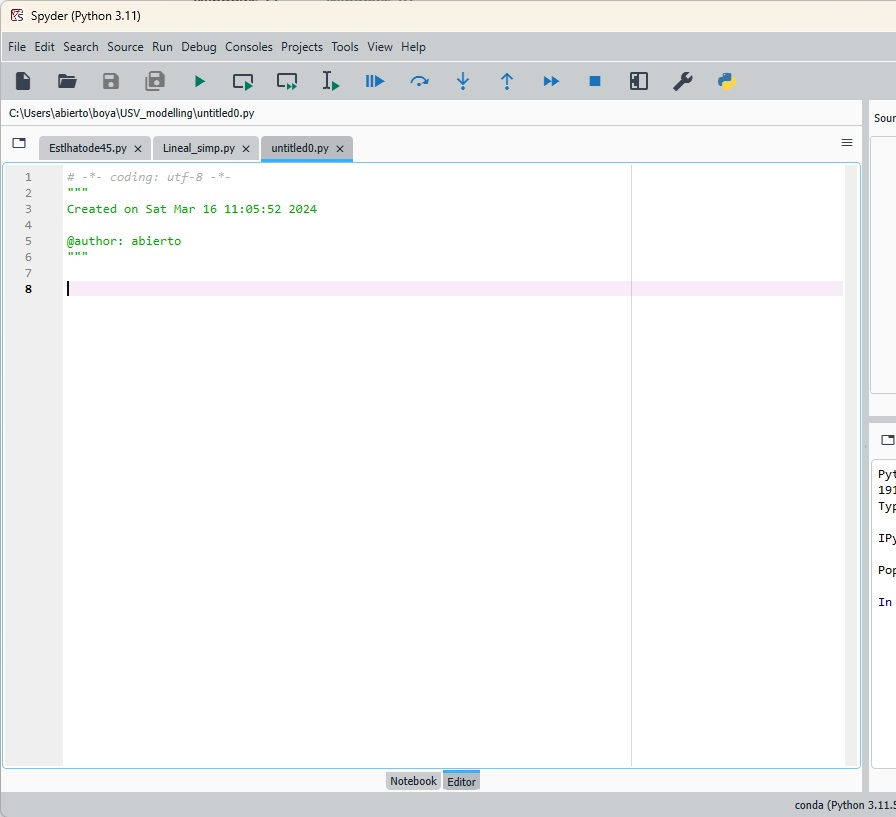
\includegraphics[width=14cm]{figuras/editor.jpg}
\bicaption{Editor de textos para Python incluido en Spyder}{Text editor for Python included in Spyder}.
\label{fig:script}
\end{figure}
    
\begin{paracol}{2}
\subsection{El editor de textos de\\ Spyder.} \index{Editor de textos}
Podemos emplear un editor de textos cualquiera, que genere texto en ASCII, como por ejemplo el 'block de notas', para escribir nuestros programas. Sin embargo, si trabajamos en el entorno de Spyder, lo ideal es emplear su propio editor de textos.

El editor de textos de Spyder ocupa el panel izquierda del la ventana del IDE, (figura \ref{fig:ide}). En la figura \ref{fig:script} se muestra una vista más detallada de este panel.

\switchcolumn

\subsection{The Spyder's text editor}\index[eng]{Text editor}
We can use whatever text editor we want to write our programs, provided it generates text in ASCII format. For instance, we can use the classical 'notepad'. Nevertheless, If we are working with Spyder, we should use its text editor.

The Spyder's text editor is located in the left panel of the IDE window (figure \ref{fig:ide}. Figure \ref{fig:script} shows a more detailed view.

\switchcolumn
La figura nos muestras un panel con varias pestañas. Cada una corresponde a un archivo de texto que contiene un programa escrito en Python. En la pestaña se indica el normbre del archivo. El archivo visible en la figura muestra el nombre \texttt{untitle0.py}. Se trata de un archivo nuevo que acabamos de abrir para escribir un nuevo programa. Para crear un nuevo Sript en Spyder basta pulsar el icono situado a la izquierda en la parte superior del panel del editor de texto o bien desplegar el menú \emph{File} situado justo encima y seleccionar la opción \emph{New file}.

Si nos fijamos en la figura \ref{fig:script}, vemos que el archivo numera en la parte derecha las líneas de código. Además aparecen ya unas líneas escritas,

Las líneas que aparecen escritas por defecto en el archivo de texto, no son comandos de Python. Se trata de comentarios. Es decir, líneas en la que damos información a quien lee el fichero sobre su contenido, autor, fecha de creación etc. Python admite dos tipos básicos de comentarios:
\begin{itemize}
    \item Líneas individuales cuyo primer carácter es una almohadilla \#. Python interpreta que toda la línea es un comentario y se la salta.
    \item Grupos de líneas encerrados entre grupos de tres comillas \verb|"""|. Se emplean para comentarios más largos, en los que se dan explicaciones más completas de lo que hace el código.
\end{itemize}
\switchcolumn
The figure shows a panel with several tabs. Each one belongs to a different text file containing a Python program. The file name is written in the tab. The file shown in the figure has the name \emph{untitle0.py}. It is a new file we have just opened to write a new program. To create a new Spyder script, it is enough to click the left icon on top of the editor panel or unfold the File menu located just above and select the option \emph{New file}.

Looking at figure \ref{fig:script}, we see how the code lines are numbered on the right side of the file how the code lines are numbered. Besides, some code lines are included.

These lines, written by default in the text file, are not Python commands; they are comments, i.e. lines that supply information on the file content to the reader. Usually, these lines contain the program's purpose, the type of variables it uses, the date of creation, the author, etc. Python accepts two kinds of comments:
\begin{itemize}
    \item Single comment lines. They start with a hash \#  symbol. Python considers the whole line a comment and skips it.
    \item A sequence of lines enclosed into groups of three quotation marks \verb|"""|. They are used for lengthier comments, which contain longer descriptions of the code performance. 
\end{itemize}
\end{paracol}


\begin{minted}[
frame=lines,
framesep=2mm,
baselinestretch=1.2,
%bgcolor=LightGray,
label=untitled0.py,
fontsize=\footnotesize,
linenos
]{python}
# -*- coding: utf-8 -*-
"""
Created on Sat Mar 16 20:05:44 2024

@author: abierto
"""
\end{minted}

\begin{paracol}{2}
En nuestro caso, Spyder nos ha escrito un comentario de línea indicando la codificación con la que se guarda el texto del archivo (\emph{utf8}). Después crea un área para un comentario del segundo tipo, (líneas 2  a 6 del código). Nos escribe la fecha en que se ha creado el archivo y el autor. Evidentemente estos valores pueden modificarse. Este espacio para comentarios creado por Python, es un buen sitio para que nosotros añadamos información sobre para qué sirve el fichero de código, el tipo e variables que define, etc.

Para seguir con el mismo ejemplo, vamos a escribir algunas líneas de código y vamos a guardar el fichero con un nombre nuevo. El fichero se guarda, bien pulsando el tercer icono por la izquierda de los que se muestran encima del panel del editor de texto, o desplegando el menú File y pulsando la opción Save as. En nuestro caso, lo vamos a guardar con el nombre \emph{ejemplo.py}.
\switchcolumn
In our case, Spyder has written a line comment showing the text codification (\emph{utf8}) used to store the file's information. Below, Spyder creates a comment area --the second type of comment-- using the code lines 2 to 6. There, it writes the file creation date and the name of the file author. Of course, this data can be changed by the user. This comment area created by Python is an excellent place to add information about the file features, the type of variables defined, etc.

We will continue with the example, adding some code lines and then save the file with a new name. To save a file, click the third icon from the left in the icon panel above the editor or unfold the File menu and select Save as. We will save our file with the name \emph{ejemplo.py}.
\end{paracol}

\begin{minted}[
frame=lines,
framesep=2mm,
baselinestretch=1.2,
%bgcolor=LightGray,
label=ejemplo.py,
fontsize=\footnotesize,
linenos
]{python}
# -*- coding: utf-8 -*-
"""
Created on Sat Mar 16 18:48:46 2024
Este Script es un simple ejemplo para mostrar el uso básico
de los Scripts de Python
This Script is a basic example just to show how to use Python's
Scripts
@author: abierto 
"""

#Primero creamos unas variables y mostramos su valor
#first we create some variables
a = [1,2,3.3,4,0,-8]
print(a)
b = 12
print(b)
c = [1,0,1,0]
print(c)
#Ahora realizamos algunas operaciones basicas con las variables
#Now we perform some basic operation with the variables created
a[3] = a[3] + 4.2
p = a.pop()
d = p+b-c[0]
#por ultimo mostramos los resultados de nuestras operaciones
#and eventually we show the resuts 
print(a)
print(p)
print(d)
\end{minted}

\begin{paracol}{2}
Si nos fijamos en los cambios introducidos. hemos añadido una líneas al comentario largo, explicando qué contiene el fichero. Además, hemos introducido comentarios de línea, explicando qué hace el código en cada paso. Es fácil ver que el programa crea dos listas \mintinline{python}{a} y \mintinline{python}{c} y una variable entera \mintinline{python}{b}. Además las imprime en el terminal para que veamos el valor que tomas. a continuación, suma $4.5$ al valor del cuarto elemento de la lista \mintinline{python}{a}, extrae el último valor de dicha lista y lo guarda en una variable nueva \mintinline{python}{p}. En la línea $23$ crea una nueva variable \mintinline{python}{d} sumando \mintinline{python}{p} y \mintinline{python}{b} y restando al resultado el último elemento de lalista \mintinline{python}{c}. Por último nos muestra el valor de las variables \mintinline{python}{a}, \mintinline{python}{p} y \mintinline{python}{d}.
\switchcolumn
Focusing on the changes, we added some lines to the long comment explaining the file's contents. Besides, we have introduced some line comments now and then, describing what the code does in each step. It is easy to check that we have created two Lists \mintinline{python}{a} and \mintinline{python}{c} and an integer variable \mintinline{python}{b}. Moreover, python prints these new variables on the console to show their values. Then, it adds $4,5$ to the current value of the fourth element of the list \mintinline{python}{a}, pops out the last values of this list and saves it in a new variable \mintinline{python}{p}. On line $23$, a new variable, \mintinline{python}{d} is created, adding  \mintinline{python}{p}and \mintinline{python}{b} and subtracting from the result the last element of the list \mintinline{python}{c}. Eventually, Python shows the values of variables \mintinline{python}{a}, \mintinline{python}{p} and \mintinline{python}{d}.

\switchcolumn
\subsection{Ejecución de scripts}
Una vez que hemos terminado de escribir nuestro código, necesitamos ejecutarlo, para obtener los resultados del programa. Dentro del entorno de Spyder, la ejecución de un script se lleva a cabo pulsando el icono señalado con un triángulo verde, situado en la parte superior del panel del script o bien seleccionando en el menún desplegable \emph{Run} la opción \emph{Run}.

Los resultados de la ejecución aparecen en la consola de Ipython,
\switchcolumn
\subsection{Running a script}
Once we have finished our code edition, we need to run it to obtain the results. Using the Spyder environment, we run a script by clicking the green triangle icon located on top of the editor panel or unfolding the Run menu and selecting the option Run.

The results are shown on the Ipython console,
\end{paracol}

\begin{minted}{python}
In [4]: runfile('C:/Users/abierto/Documents/borrar/ejemplo.py', 
wdir='C:/Users/abierto/Documents/borrar')
[1, 2, 3.3, 4, 0, -8]
12
[1, 0, 1, 0]
[1, 2, 3.3, 8.2, 0]
-8
3
\end{minted}
\begin{paracol}{2}
En realidad, al pulsar el icono de ejecución, lo que hacemos es ejecutar el comando \mintinline{python}{runfile()}, indicando entre paréntesis el fichero que queremos que se ejecute. además, la consola de Ipython muestra los resultados de los comandos \mintinline{python}{print} que hemos definido en nuestro programa. A efectos prácticos, ejecutar el script es equivalente a escribir sus líneas de código una a una en la consola. De hecho, Python ha guardado en memoria las variables que hemos creado, de modo que podemos usarlas si introducimos nuevos comandos en la consola. Por ejemplo, podemos añádir un nuevo elemento al final de las lista \mintinline{python}{c},
\begin{minted}{python}
 In [7]: c.append(31.2)
In [8]: print(c)
[1, 0, 1, 0, 31.2]

In [9]:    
\end{minted}
\switchcolumn
When we click the icon Run, we execute the command \mintinline{python}{runfile()}, including, enclosing in parentheses, the name of the file we want to run. Then, Python shows the results of the \mintinline{python}{print} command that we have included in our program. From the point of view of the results, there is no difference between running the script or writing their lines one by one in the Ipython console. In fact, Python has saved the variables we created running the script in the computer memory, and we can use them if we introduce new commands in the console. For instance, we can add a new element at the end of list \mintinline{python}{c},
\begin{minted}{python}
 In [7]: c.append(31.2)
In [8]: print(c)
[1, 0, 1, 0, 31.2]

In [9]:    
\end{minted}
\end{paracol}
\begin{paracol}{2}

\section{Funciones en Python} \index{funciones}
en la sección anterior hemos visto como emplear scripts para guaradr nuestro código y poder reutilizarlo siempre que queramos. Aunque esto supone una mejora respecto a reescribir nuestros comandos de nuevo en la consola, todavía da lugar a código poco flexible y reutilizable. Vamos a introducir en esta sección una estructura de programación que va hacer de nuestro código una herramienta mucho más potente. Se trata de las funciones.

En Python podemos definir funciones directamente en la consola, pero esto no es, en general, una buena idea; cuando cerramos Spyder perdemos el trabajo hecho. Vamos por tanto a utilizar scripts para definir nuestras funciones.

La estructura general de una función en python toma la siguiente forma

\begin{minted}{python}
def nombre_de_la_funcion(e1,e2,...):
    código de la función
    return, r1, r2, ...
\end{minted}

La primera línea de la definición de una función recibe el nombre de cabecera. La cabecera de la función empieza siempre con la palabra clave \mintinline{python}{def}. A continuación se indica el nombre que tendrá la función. Los nombre válidos deben empezar por letras y en general no es buena idea emplear caractéres especiales. A continuación, entre paréntesis y separadas por comas se incluyen las variables de entrada, es decir, aquella variables que la función va  a emplear para realizar sus cálculos. Si no necesita tomar variables de entrada, se deja es paréntesis vacío, pero no se omite. Por último se añade el símbolo ':' para indicar que se ha terminado de definir la cabecera de la función.

Debajo de la cabecera, viene las líneas de código de la función, que constituyen el cuerpo de la misma. Una caracterítica importante de Python es que todas las líneas de código pertencientes a una función deben estar indentadas, es decir, deben empezar dejando un número igual de espacios en blanco al principio de todas las lineas. Una de las ventajas de emplear el editor de textos de Spyder es que, si definimos una línea de cabecera correctamente,  y pulsamos la tecla intro, directamente nos indenta las líneas siguientes. La última línea duna función suele emplearse para devolver variables que contienen los resultados que desamos optener de las operaciones realizadas por la función. Empieza con la palabra clave \mintinline{python}{return} y va seguida de una lista de variables separadas por comas. Por supuesto dichas variables se tienen que haber definido antes en las líneas de código de la función. A continuación vamos a ver un ejemplo de una función construida para obtener las soluciones de una ecuación de segundo grado,
\begin{equation*}
    ax^2+b^x+c = 0
\end{equation*}
Cuyas soluciones toman la forma general,
\begin{equation*}
    x_{1,2} = \frac{-b\pm \sqrt{b^2-4ac}}{2a}
\end{equation*}
\switchcolumn
\section{Functions in Python} \index[eng]{functions}
In the previous section, we learned about using scripts to save our code and reuse it later. While this is an improvement over repeatedly rewriting the same commands in the console, it still results in code that is not very flexible and reusable. In this section, we will introduce functions, a programming structure that enables our code to become a more powerful tool.

In Python, it is possible to define functions using the console. However, this is not advisable because all work will be lost once Spyder is exited. takes in Python the following general structure,

\begin{minted}{python}
def funcion_name(e1,e2,...):
    function code
    return, r1, r2, ...
\end{minted}
\begin{equation*}
    ax^2+b^x+c = 0
\end{equation*}

The first line of a function definition is known as the function header. It always starts with the keyword \mintinline{python}{def}. Following this, we write the name of the function. Valid function names follow the same rules as file names. After the function name, we enclose input variables in parentheses, separated by commas. These input variables are the variables that the function will use to perform its operations. When the function does not need input variables, we leave the parentheses empty but never omit them. Eventually, we write the symbol ':' to end the function header.

Beneath the header file comes the function body, that is, the code lines of the function. One important feature of Python language is that any line belonging to the body function should be indented. The function body lines should begin, leaving the same number of blank spaces from the beginning of the line. One advantage of using the Spyder text editor is that it automatically acknowledges the file header lines and indents the following lines. The last function line is usually used to recover variables that contain the function operations' relevant results. It starts with the keyword \mintinline{python}{return}, followed by a list of variables separated by commas. These variables should be defined in the function body.

Let's look at an example function for solving quadratic equations.
\begin{equation*}
ax^2+bx+c=0
\end{equation*}

it has the following general solutions,
\begin{equation*}
    x_{1,2} = \frac{-b\pm \sqrt{b^2-4ac}}{2a}
\end{equation*}
\end{paracol}

\begin{minted}[
frame=lines,
framesep=2mm,
baselinestretch=1.2,
%bgcolor=LightGray,
label=eq\_seg\_grado.py,
fontsize=\footnotesize,
linenos
]{python}
# -*- coding: utf-8 -*-
"""
Created on Mon Mar 18 18:33:43 2024
Este script contiene una función para obtener la solucion de una 
ecuación de segundo grado.
This script defines a function to solve a quadratic equation
@author: abierto
"""
def soleq2(a,b,c):
    """
    Esta función calcula las soluciones de la ecuación general,
    ax**2 + b*x + c = 0
    Variables de entrada:
        coeficientes a, b y c
    Variables de salida:
        xp Solucion para la raíz cuadrada positiva
        xm solucion para la raiz cuadrada negativa
        
    this function calculates the solutions of the general equation
    a*x**2 + b*x + c = 0
    input variables:
        a,b and c coeficients
    output variables;
        xp solution using positive square root
        xm solutions using negative square root
    """
    xp = (-b+(b**2-4*a*c)**(1/2))/2/a
    xm = (-b-(b**2-4*a*c)**(1/2))/2/a
    return xp, xm

#aquí añadimos un ejemplo de uso que no es parte de la funcion
#here we add a 'how to use' example that's not part of the function

solplus, solminus = soleq2(2, 3, 1)

#comprobacion
#checking
print('raíz positiva/positive root:', 2*solplus**2+3*solplus+1)
print('raiz negativa/negative root:', 2*solminus**2+3*solminus+1)
\end{minted}

\begin{paracol}{2}
    Para definir nuestra función hemos abierto un nuevo script en el editor de texto de Spyder y lo hemos guardado con el nombre \texttt{eq\_seg\_grado.py}. Evidentemente, se puede guardar con cualquier nombre, aunque es buena costumbre tratar de buscar uno que nos de alguna pista de qué contiene el script.

    Tras, incluir un breve comentario sobre el contenido del fichero, hemos definido la cabecera de la función en la línea $9$. Es interesante fijarse en la definición: el nombre de la función es \mintinline{python}{soleq2}, y ha continuación, entre paréntesis hemos definido como variables de entrada los tres coeficientes de la ecuación que queremos resolver. Cerramos la cabecera, añadiendo el símbolo 'dos puntos' final. Inmediantamente debajo, de la cabecera, hemos incluido un comentario amplio, describiendo qué hace la función cuáles son sus variables de entrada, y qué variables, con los resultados, nos va a devolver.

    La línea $27$ contiene las operaciones matemáticas para obtener la solución de la ecuación correspondiente a la solución con raíz cuadrada positiva y guarda le resultado en la variable \mintinline{python}{xp}, mientras que la línea $28$ contiene la solución  correspondiente a la raíz cuadrada negativa y guarda el resultado en la variable \mintinline{python}{xm}. ¡Compruébalo!
    Por último la línea $29$ devuelve las variables \mintinline{python}{xp,xm} con los resultados calculados.

    Aquí termina la definición de la función. Por eso, las líneas siguientes de código, que no forman parte de la función, no están indentadas. Las hemos añadido simplemente para mostrar cómo utilizar la función \mintinline{python}{soleq2} y comprobar que los resultados son correctos.

    En la línea $34$ se muestra cómo emplear (llamar) a la función que acabamos de crear. En primer lugar definimos dos variables en los que guardar los resultados \mintinline{python}{solplus} y \mintinline{python}{solminus}. Python asociará, por orden, estas variables separadas por comas, a las varibles definidas tras la palabra clave \mintinline{python}{return}. Es decir, copiará el contenido de la variable \mintinline{python}{xp} en la variable \mintinline{python}{solplus} y el de la variable \mintinline{python}{xm} en la variable \mintinline{python}{solminus}. Evidentemente, podemos elegir cualquier nonmbre de variable válido para guardar los resultados. A continuación escribimos el símbolo de asignación $=$, seguido del nombre de la función. Por último, damos valores a las variables de entrada \mintinline{python}{a,b,c}.

     Las líneas $38$ y $39$ comprueban que las dos raíces obtenidas satisfacen la ecuación de segundo grado, $2x^2+3x+1 = 0$. Hemos añadido al comando \mintinline{python}{print}, un texto entre comillas para que nos indique qué resultado de las comprobaciones corresponde a cada solución obtenida.

     Si ejecutamos el script que hemos creado, pulsando el icono con el triángulo verde, Obtenemos en la consola de Ipython el siguiente resultado,
     \switchcolumn
     We have opened a new script in the Spyder text editor to define our function. We have saved the Script with the name {eq\_seg\_grado.py}. Obviously, you can save the file with whatever valid name you like, but it is a good idea to find a name that gives us some hints in the script content (quad\_eq.p should be a nice name for this script). 

     After briefly commenting on the file's content, we define the function header on line number $9$. It is interesting to look carefully at this definition: After writing the keyword \mintinline{python}{def}, we have given a name to the function \mintinline{python}{soleq2,} and, next, we have defined the input variables, enclosed in parentheses and separated by commas. These input variables will be the coefficients of the quadratic equation we wish to solve. We close the function header, adding the final colon. Just beneath the header, we have added a rather lengthy comment explaining the purpose of the function and describing its input and output variables.

     We have written the mathematical operations for the quadratic equation's positive and negative squared roots in lines 27 and 28, respectively. Check it! In the first case, we have saved the result in variable \mintinline{python}{xp} and, in the second case, we have saved the result for the negative squared root in variable\mintinline{python}{xm}. Lastly, line number $29$ returns variables \mintinline{python}{xp, xm} with the operation results.

     The function definition finishes here. The remaining code lines do not belong to the function, so they are not indented. We have added them to show how to use the function \mintinline{python}{soleq2} and check if the results are correct.

     In line $34$, we show how to use (call) the already created function. First, we define two variables, \mintinline{python}{solplus} and \mintinline{python}{solminus} for saving the function results.
     These variables, separated by commas, are orderly associated with those returned by the function,i.e. the variables included in the function code after the keyword \mintinline{python}{return}. Thus, Python will copy the content of variable \mintinline{python}{xp} in variable \mintinline{python}{solplus} and the content of variable \mintinline{python}{xm} in variable \mintinline{python}{solminus}. It is unnecessary to say that we can give whatever valid name we want to the variables we use to save the function results. After the variables above, we write the assignation symbol followed by the function name. lastly, we write values for input variables, \mintinline{python}{a,b,c}.

     Lines $38$ and $39$ check that both obtained solutions fulfil the quadratic equation $2x^2+3x+1 = 0$. We have added a quoted text to the \mintinline{python}{print} command that helps to determine which result is up to each solution.

     If we click on the green triangle icon and run the script we have written, we get the following result in the Ipython console,
     
\end{paracol}

\begin{minted}{python}
In [1]: runfile('C:/Users/abierto/boya/USV_modelling/eq_seg_grado.py',
wdir='C:/Users/abierto/boya/USV_modelling')
raíz positiva/positive root: 0.0
raiz negativa/negative root: 0.0

In [2]:    
\end{minted}

\begin{paracol}{2}
Es importante recordar que un script no es más que una secuencia de instrucciones que se ejecutan en el terminal. Por tanto, si seguimos la secuencia del script del ejemplo, lo primero que hemos hecho es \emph{crear} la función que hemos definido y guardarla en la memoria del ordenador. Por eso, podemos ahora si quemeremos seguir utilizándola directamente en el terminal,
\switchcolumn
It is important to note that a script is just a sequence of instructions that run in the console. Thus, if we track the sequence of the example script, we first \emph{create} the function defined in the script and save it in the computer memory. Hence, as long as we don´t quit Spyder,  we can keep on using it directly in the Ipython terminal,  
\end{paracol}

\begin{minted}{python}
In [12]: coef = [3,-2,2]
In [13]: sp, sm = soleq2(coef[0],coef[1],coef[2])
In [14]: print(sp)
(0.3333333333333334+0.7453559924999299j)
In [15]: print(sm)
(0.3333333333333333-0.7453559924999299j)
In [16]: print(solplus)
-0.5
In [17]: print(solminus)
-1.0   
\end{minted}

\begin{paracol}{2}
En este caso, hemos agrupado los coeficientes de la ecuación de segundo grado que queremos resolver en una lista \mintinline{python}{coef}. Despues, llamamos a la función. El procedimiente es el mismo de antes, definimos unas variables de salida para guardar los resultados \mintinline{python}{sp, sn} escribimos el signo de asignación, el nobre de la función y damos valores a las variables de entrada. Tal y como las hemos escrito, la función identificará el coeficiente \mintinline{python}{a} con el primer elemento de la lista \mintinline{python}{coef[0]}, el segundo con coeficiente con el segundo elemento de la lista, etc.

A continuación empleamos el comando \mintinline{python}{print}, para observar los valores de las variables de salida. En esta caso, la equación no tiene soluciones reales, y el resultado son dos números complejos conjugados.

Las dos últimas líneas In[16] e In[17] las hemos empleado para imprimir el valor de las variables \mintinline{python}{solplus} y \mintinline{python}{solminus}. Esta variables se crearon cuando se ejecutó el script, pero Python las conserva todavía en memoria.
\switchcolumn
Notice that we have collected the quadratic equation coefficients in a Python list in this example. Then, we call the function. The procedure is the same as before; we define output variables to save the results \mintinline{python}{sp, sn}, write the assignation symbol and the function name and give values to the input variables. These last have been written so that the function should identify the quadratic equation \mintinline{python}{a} coefficient with the first element of the list, the second coefficient with the second element of the list, etc. 

Next, we use the command \mintinline{python}{print} to watch the output values of the output variables. In this case, the equation does not have real solutions, and the results are two complex conjugated numbers.

The last two lines, In[16] and In[17], are used to show the value of \mintinline{python}{solplus} and \mintinline{python}{solminus}. these variables were created when we ran the script, but Python still holds them in the computer memory. 
\switchcolumn
\section{Los \emph{Namespace} en Py\-thon y el ámbito de las variables} \index{Namespace}\index{Variable!Ambito}
Acabamos de ver que python conserva en la memoria las variables creadas para emplearlas posteriormente. Es importante entender cómo python lleva a cabo la gestión de las variables creadas en memoria. Esto nos lleva al concepto de \emph{namespace}.
Por \emph{namespace} entendemos un espacio de memoria, reservado por Python donde los programas y funciones puedes acceder para buscar variables, funciones y, en general, objetos de programación.

En Python se definen cuatro \emph{namespaces} diferentes. Su definición es dinámica, es decir, tienen una duración en tiempo límitada: se crean cuando son neceserios y se destruyen una vez que que una vez que dejan de ser necesarios. Habitualmente varios \emph{namespaces} coexisten a la vez. Veamos cuales son:

\switchcolumn
\section{Namespace and Scope in Python}
We have seen that Python holds the created variables in the computer memory so that they can be used later. Understanding how Python manages the variables saved in the computer memory is essential. This takes us to the idea of Python \emph{namespaces}.
A \emph{namespace} could be considered a memory space reserved by Python, where programs and functions can access to find variables, functions and, in general, programming objects.

Python defines four different \emph{namespaces}. They are dynamically defined, meaning they last for a limited time. They are created when necessary and destroyed when they are no longer needed. Usually, several \emph{namespaces} coexist. They are:

\switchcolumn
\paragraph{Built-in Namespace.} Contiene todas las variables y funciones propias de Python. Dichas variables son accesibles siempre que tenemos abierta una consola de Python. Podemos listar sus nombres escribiendo en la consola de Python el comando \mintinline{python}{dir(__builtins__)}. Por ejemplo, la función \mintinline{python}{print}, pertenece a este \emph{namespace}. Podemos acceder a las funciones y variables contenidas en Built-in, desde cualquier función o programa de Python.

\paragraph{Global namespace.} Podríamos decir que este \emph{namespace} contiene todas las variables y funciones que hemos definido en un script. Sin embargo, para entender mejor a qué nos estamos refiriendo es preciso introducir el conceptos de importación. Volvamos por un momento al ejemplo que vimos más arriba en el que creamos un script que contenía una función \mintinline{python}{soleq2} que calculaba las soluciones de una ecuación de segundo grado. Hemos visto que si ejecutamos el script, en Spyder la función quedaba en la memoría del ordenador y podíamos emplearla para resolver cualquier ecuación de segundo grado directamente en la consola de Ipython.

Pero, ¿Qué pasa si queremos emplear dicha función en otro script? ¿Debemos volver a escribirla de nuevo? La respuesta es no. Para emplear la función \mintinline{python}{soleq2}, podemos \emph{importar} nuestro primer script en el segundo mediante el comando \mintinline{python}{import}. Veamos un ejemplo, 

\switchcolumn
\paragraph{Built-in Namespace.} This namespace stores all Python Built-in variables and functions. We can access these variables whenever we have a Python terminal opened. We list their names by writing the command \mintinline{python}{dir(__builtins__)} on the Ipython terminal. For instance, the function \mintinline{python}{print} belongs to this \emph{namespace}. We can access every function and variable stored in the Built-in namespace from whatever function or program we write in Python.

\paragraph{Global Namespace.} We could say that this \emph{namespace} contains all functions and variables defined in a script. Nevertheless, we will introduce the importation concept to understand better what we mean by this. Let's return to the example above, where we wrote a script with a function \mintinline{python}{soleq2}, allowing us to get a quadratic equation's roots. We have seen that if we run the script in Spyder, the function \mintinline{python}{soleq2} is stored in the computer memory, and we can use it straightforwardly on the Ipython terminal to solve any quadratic function.

But what if we want to use the function \mintinline{python}{soleq2} in another script? Do we need to write down the equation again in the new script? The answer is not. Python supplies a method to access the functions and variables of one script from another. The method is known as \emph{importation}; we import one script into another using the command \mintinline{python}{import}. The following script shows an example, 
\end{paracol}

\inputminted[
frame=lines,
framesep=2mm,
baselinestretch=1.2,
%bgcolor=LightGray,
label=Example\_import.py,
fontsize=\footnotesize,
linenos
]{python}{./codigos/introduccion/codigo_abierto/Example_import.py}

\begin{paracol}{2}
La línea $10$ de ejemplo \mintinline{python}{Example_import.py}, usa el comando \mintinline{python}{import} para \emph{importar} el contenido del script \mintinline{python}{eq_seg_grado.py}. Importante: se escribe el nombre del archivo sin la extensión \mintinline{python}{.py}. Cuando se ejecuta esta línea de código, se ejecuta el script \mintinline{python}{eq_seg_grado.py} y se crea un namespace global que contiene todas las funciones y variables creadas por dicho script.

En las líneas $11-13$ definimos tres variables, para usarlas como coeficientes de una equación de segundo grado y en la línea $14$ llamamos a la función \mintinline{python}{soleq2} para resolver dicha ecuación. Esta función está contenida en el namespace global de \mintinline{python}{eq_seg_grado.py}, para acceder a ella escribimos:
\mint{python}{eq_se_grado.soleq2}
Es decir: primero indicamos el namespace y, separado por un punto, el nombre de la función. Esta es la forma en que podemos acceder a cualquiera de las funciones o variables definidas en un script a través de otro script.

¿por qué definir las variables y funciones en namespaces separados? Una razón es que permite repetir nombres de variables y funciones en distintas partes de nuestro código sin que accidentalmente unos borren a otros. En el ejemplo anterior, en la línea $14$ hemos guardo los resultados de las soluciones de la ecuación de segundo grado en las variables \mintinline{python}{solplus} y \mintinline{python}{solminus}. Pero estos nombres de variable ya existían. Hemos dicho que al importar \mintinline{python}{eq_seg_grado}, este script se ejecuta. Si revisamos sú codigo, vemos que en la línea $34$ \mintinline{python}{solplus, solminus = soleq2(2, 3, 1)}, Se llama a la función \mintinline{python}{soleq2}, y se emplean exáctamente los mismos nombres de variable para guardar los resultados. Aunque ambos resultados se guardan con los mismos nombres, pertenecen a namespaces distintos. Si ejecutamos el script \mintinline{python}{Example_import.py} obtenemos en el terminal de Ipython los siguiente resultados,

En términos generales, cuando se importa un script, lo que se crea es una estructura de programación, que en Python se conoce con el nombre de módulo. El módulo toma el nombre del script que lo genera, exceptuando la extensión. Para acceder a las funciones contenidas en el módulo, basta anteponer al nombre de la variable o función el nombre del módulo separado por un punto.

Si descontamos las funciones y variables definidas en el Built-in, todo el resto de código escrito en Python, está pensado para crear módulos. Lo habitual es que estos módulos se agrupen en paquetes de software que engloban funciones y objetos orientados a tareas específicas. A lo largo de estos apuntes, veremos algunos de ellos como numpy, orientado al cálculo científico o matplotlib, dedicado a la realización de gráficos.
\switchcolumn
Line number $10$ on \mintinline{python}{Example_import.py} example, uses the command \mintinline{python}{import} to \emph{import} the content of script \mintinline{python}{eq_seg_grado.py}. Attention: we write the name of the file without the extension \mintinline{python}{.py}. When program line number $10$ is executed, the script \mintinline{python}{eq_seg_grado.py} is thoroughly executed, and a global namespace is created to save the variables and functions created by this script.

In lines $11 - 13$, we define three variables to be used as coefficients for a quadratic equation. Later, in line $14$, we call function \mintinline{python}{soleq2} to solve the equation. But \mintinline{python}{soleq2} belongs to the global namespace created when the script \mintinline{python}{eq_seg_grado} was imported. So, to access it, we write:
\mint{python}{eq_se_grado.soleq2}
We indicate the namespace first and then the function name, separated by a point. This is how we access the variables and functions defined in one script from another script. 

Why is it convenient to define variables and functions in separated namespaces? One reason is that it allows repeating the same variable and function names in different locations of our code, avoiding them clashing accidentally. In the last example, in line $14$, we saved the quadratic equation solutions in variables \mintinline{python}{solplus} y \mintinline{python}{solminus}. But these variable names have already been used. We said that we were running it when we imported \mintinline{python}{eq_seg_grado}. If we review the code of this script we can see that in line $34$\\ \mintinline{python}{solplus, solminus = soleq2(2, 3, 1)},\\ the program calls \mintinline{python}{soleq2} and the results are saved in variables with identical names,\\ \mintinline{python}{solplus} y \mintinline{python}{solminus}. Although we are saving the solutions in both cases with the same names, they belong to different namespaces. After running the script \mintinline{python}{Example_import.py}, we achieve the following result,   

Generally, a programming structure is created whenever we import a script. In Python, these program structures are called modules. A  script and the module generated when the script is imported share the same name (except for the extension). To access the functions and 
variables held in the module, it is enough to put the name of the module before the name of the function or variable separated with a point.

Except for the functions and variables defined in the Built-in namespace, the remaining code written in Python is intended to create modules. Usually, the modules are grouped into software packages which enclose functions and programming objects devoted to specific tasks. In these lecture notes, we will meet some of them, like numpy, oriented to scientific computing or matplotlib, devoted to graphical representation.    
\end{paracol}

\begin{minted}{python}
In [1]: runfile('C:/Users/abierto/Documents/borrar/Example_import.py',
wdir='C:/Users/abierto/Documents/borrar')
raíz positiva/positive root: 0.0
raiz negativa/negative root: 0.0
Example_import: 1.7071067811865475
Example_import: 0.2928932188134524
eq_seg_grado: -0.5
eqseg_grado: -1.0

In [2]: 
\end{minted}
\begin{paracol}{2}
Al importar \mintinline{python}{eq_seg_grado}, se ejecuta dicho script. Se calcula por tanto la solución de la ecuación de segundo grado: $x^2+2x+3=0$ y se muestran en el terminal las comprobaciones de los resultados. Una vez terminada la importación, todas las variables y funciones creadas por \mintinline{python}{eq_seg_grado}, están disponibles en su namespace global. despues, observamos en el terminal los resultados de las dos ecuaciones de segundo grado resueltas. Las dos primeras, corresponden a la ecuación $2x^2+3x+1=0$, y las dos últimas a la ecuación $x^2+2x+3=0$. Para imprimir estas últimas, hemos empleado \mintinline{python}{eq_seg_grado.solplus}\\
\mintinline{python}{eq_seg_grado.solminus},\\ 
para indicar que nos referimos a las variables guardadas en el namespace de \mintinline{python}{eq_seg_grado}.
\switchcolumn
As we have already said, this script is run when we import \mintinline{python}{eq_seg_grado}. Thus, the program calculates first the solution of the quadratic function: $x^2+2x+3=0$ and shows the checking of the solutions on the Ipython terminal. Once the importation is over, all created functions and variables are available in the script's global namespace. Then, we see the results of the two quadratic equations solved on the Ipython terminal. First, the solutions of    $2x^2+3x+1=0$ and then the solutions of $x^2+2x+3=0$. To print these last solutions, we use\\
\mintinline{python}{eq_seg_grado.solplus}\\ 
\mintinline{python}{eq_seg_grado.solminus},\\
To indicate that, we want to print the variables held in the global namespace \mintinline{python}{eq_seg_grado}.  

\switchcolumn
\paragraph{Local Namespace.} Este \emph{namespace} es propio de las funciones. Cuando se ejecuta una función en Python, se crea un  namespace específico (local)  para dicha función en la que se guardan las variables que la función crea y utiliza durante su ejecución. Una vez que la funcion termina, el namespace local asociado se destruye, y las variables dejan de estar accesibles.

Si nos fijamos en el código de la función \mintinline{python}{soleq2}, vemos que la función crea unas variables \mintinline{python}{a,b,c} en su cabecera. Dentro de la función se emplean dichas variables para resolver una equación de segundo grado, y se guardan las soluciones en las variables \mintinline{python}{xp,xm}. Estas cinco variables pertenecen al namespace local de la función \mintinline{python}{soleq2} y solo el código de dicha función puede acceder a ellas.

Cuando llamamos a la función \mintinline{python}{soleq2} tanto si lo hacemos desde un módulo como desde la línea de comandos, empleamos el signo de asignación para copiar las variables de salida y damos valores a las variables de entrada. Por ejemplo si nos fijamos en la línea $14$ del módulo \mintinline{python}{Example_import.py},
\switchcolumn
\paragraph{Local Namespace.} This \emph{namespace} is used by Python functions. Whenever a function is executed, a specific namespace (local) is created for the function. Every variable created by the function is saved in its local namespace, and it is available for the function to use during execution. Once the function ends, its associated local namespace is destroyed, and the variables are no longer accessible.

Focus on function \mintinline{python}{soleq2} code, we can see how the function creates variables \mintinline{python}{a,b,c} in its header. In the function body, these variables are used as the coefficients of the quadratic function to be solved. The solutions are saved in variables \mintinline{python}{xp,xm}. These five variables belong to the local namespace of the function \mintinline{python}{soleq2}, and only this function code can access them. 

When we call function \mintinline{python}{soleq2}, whether from another module or the command line, we use the assignation symbol to copy the output variables and give values to the input variables. For instance, recall the line number $14$ of the \mintinline{python}{Example_import.py} module,
\end{paracol}
\mint{python}{solplus, solminus = eq_seg_grado.soleq2(e, f, g)}
\begin{figure}[h]
\centering
\begin{tikzpicture}
%\usetikzlibrary{shapes.multipart}
\path(0,0) node(a) [rectangle split,rectangle split parts =2,draw=blue,top color=white,bottom color=blue!15, very thick,align=center,rounded corners]{Built-in Namespace \hspace{200pt}
\nodepart{two}
\ \\
\vspace{200pt}
\ \\
Python
}		
(0,0) node(b)[rectangle split,rectangle split parts =2,draw=yellow, top color=white, bottom color=yellow!15,thick,rounded corners,align=left]{Global Namespace \hspace{150pt}
\nodepart{two}
\ \\
\vspace{150pt}
\ \\
Módulos/Modules
}
(0,0) node(c)[rectangle split,rectangle split parts =2,draw=teal,top color=white, bottom color=teal!15,thick,rounded corners,align=left]{Enclosing Namespace \hspace{100pt}
\nodepart{two}
\ \\
\vspace{100pt}
\ \\
Funciones/Functions
}
(0,0) node(d)[rectangle split,rectangle split parts =2,draw=red,top color=white, bottom color=red!15,align=left,very thick, rounded corners]{Local Namespace \hspace{50pt}
\nodepart{two}
\ \\
\vspace{10pt}
\ \\
Funciones dentro de funciones\\
Functions inside functions
\vspace{30pt}
};
\end{tikzpicture}
\bicaption{Relación de inclusión entre los Namesapces de Python}{Inclusion relationship among Python Namespaces}
\label{fig:amb}
\end{figure} 

\begin{paracol}{2}
El contenido de las variables \mintinline{python}{e,f,g}, que pertenecen al namespace global del módulo \mintinline{python}{Example_import.py} en qué se llama a la función, se copian en las variables \mintinline{python}{a,b,c} que pertenecen al namespace local de la función. Cuando se ejecuta el comando \mintinline{python}{return} el valor de las variables \mintinline{python}{xp,xm} que pertenecen al namespace local de la función, se copian en las variables\mint{python}{solplus, solminus} que pertenecen al namespace global del módulo \mintinline{python}{Example_import.py}.

\paragraph{Enclosing namespace.} En ocasiones, llamamos a una función desde dentro de  otra función. Por ejemplo nuestra función \mintinline{python}{soleq2}, llama a la función \mintinline{python}{print}, que pertenece al namespace Built-in the Python. Cuando se ejecuta la funcion \mintinline{python}{soleq2}, ésta crea su propio namespace, y cuando dentro de ésta se ejecuta la función \mintinline{python}{print} esta última tambien crea su propio namespace local, dentro del namespace de la función \mintinline{python}{soleq2}. Se dice entonces que el namespace local de \mintinline{python}{soleq2} \emph{encierra} al namespace de \mintinline{python}{print}. 
En general, cuando una función llama a otra, El namespace de la primera se considera el Enclosing namespace de la segunda. El porqué de esta definición se entiende mejor explicando el concepto de ámbito de una variable.
\switchcolumn
When the function is called, variables \mintinline{python}{e,f,g}, which belong to the global namespace of the modules \mintinline{python}{Example_import.py} are copied in variables  \mintinline{python}{a,b,c}, which belong to the function local namespace. When the function at the end executes the command \mintinline{python}{return}, the values of variables \mintinline{python}{xp,xm}, which belong to the local namespace of the function, are copied in variables \mint{python}{solplus, solminus}, which belong to the global namespace of module \mintinline{python}{Example_import.py}.

\paragraph{Enclosing namespace.} Sometimes, we call a function from inside another function. So, our function \mintinline{python}{soleq2}calls to función \mintinline{python}{print}, which belongs to the Python Built-in namespace. When function \mintinline{python}{soleq2} is executed, it creates its own namespace and when inside it function, \mintinline{python}{print} is executed this last, also creates its own local namespace inside the namespace of \mintinline{python}{soleq2}. The local namespace of \mintinline{python}{soleq2} \emph{encloses} the namespace of \mintinline{python}{print}. 
In general, when a function calls another, the namespace of the first function is considered the Enclosing namespace of the second function. The reason for this name may be better understood by explaining the concept of variable scope.

\switchcolumn
\paragraph{Ámbito.}\index{Ámbito de una variable o función} Acabamos de describir el concepto de \emph{namespace} como una región de memoria, asociada a un módulo o a una función. La existencia de distintos namespace, hace que no todas las variables y/o funciones puedan se manipuladas desde cualquier lado. El ámbito de una variable o función define las funciones, módulos, etc desde lo que es posible acceder y manipular dicha variable o función. Los ámbitos, están fuertemente relacionados con las namespace y en python se cumple una regla general conocida como la regla "LEGB" (Local->Enclosing->Global->Built-in). Nos da, el orden de precedencia de los namespace. Así, una función tiene acceso a todas sus variable y funciones locales (Local namespace) a todas las de la función que la ha llamado, si es el caso (Enclosing namespace), a todas las del módulo que ha llamando a la función (Global namespace) a todas las del Built-in namespace. También se cumple lo contrario: desde la línea de comando solo se tiene acceso a las variables que se han creado en la propia línea de comando. Desde ún módulo se tiene acceso a las variables y funciones built-in y pero no a las de las funciones contenidas en el módulo.
Desde una función se tiene acceso al contenido Built-in y al del módulo y, en su caso, la función, que contiene la función, pero no al de las funciones, contenidas o llamadas en dicha función.
La fígura \ref{fig:amb}, muestra un esquema con el anidamiento de los namespaces en Python.
\switchcolumn
\paragraph{Scope} \index[eng]{Varaible and function scope} We have described the concept of \emph{namespace} as a memory area linked to a Python module or function. The namespaces make sure that not all variables or functions can be handled from everywhere. The scope of a variable or a function defines which functions, modules, etc., can manipulate such variable or function. The scopes are tightly related to namespaces. There is the rule known as the "LEGB" rule (Local->Enclosing->Global->Built-in) that establishes the namespace precedence order. So, a function has access to all its local variables and function (Local Namespace), to all ones belonging to the function that calls it, if any  (Enclosingnamespace), to all ones belonging to the module that calls the function (global namespace) to all builtin namespace variables and functions. It is also true that if we follow the opposite direction from the command line, we can only access built-in variables and variables created from the command line itself. From a module, we have only access to variables and functions built-in or created from the module but not to variables belonging to functions contained in the module.
From a function, access is granted to built-in variables, those belonging to the module that contains the function, those belonging to the function that includes the function, if any, and those belonging to the function itself. However, a function has no direct access to variables belonging to functions contained in or called from the function.
Figure \ref{fig:amb} shows a schematic view of Python namespace nesting.
\switchcolumn
\paragraph{Más sobre el comando \mintinline{python}{import}.}\index{import} El comando \mintinline{python}{import}, es quizá de los más empleados en Python. Más arriba hemos descrito su uso para importar un módulo entero en un script. Sin embargo, es posible emplearlo de otras muchas maneras:
\switchcolumn
\paragraph{More on \mintinline{python}{import} command.}\index[eng]{import} The \mintinline{python}{import} command is widely used in Python programming. We have already described how to use it to import a whole module. Nevertheless, it is possible to use it in very many different ways,
\end{paracol}

\begin{minted}[linenos]{python}
import eq_sec_grado
import eq_sec_grado as sec
from eq_sec_grado import *
from eq_sec_grado import soleq2
from eq_sec_grado import soleq2 as cuqui
\end{minted}

\begin{paracol}{2}
En todos los casos, el módulo desde el que se realiza la importación es el mismo, pero el modo de hacerlo es lo que cambia. Así en la línea $1$ del ejemplo importamos el módulo entero, la forma de acceder a las variables y funciones del módulo, es a través de su namesapce global: \mintinline{python}{eq_sec_grado.soleq2}. En la línea $2$, también estamos importando el módulo completo, pero ahora, usamos un 'alias', \mintinline{python}{sec},  para el nombre del namespace asociado. Esto quiere decir que para acceder a las variables y funciones del módulo debemos ahora emplear el alias en lugar del nombre del módulo: \mintinline{python}{sec.soleq2}. En la línea $3$ no importamos propiamente el módulo. Lo que hacemos es importar todas las funciones y variables contenidas el el módulo. De este modo no tenemos ya que anteponerles el nombre del módulo para usarlas. Es muy importante ser muy cuidadoso cuando se hace una importanción así. Si en el script que ha importado el módulo hay funciones y/o variables que cuyo nombre coincida con alguno de los importados, tendremos un conflicto de nombres y solo prevalecerá el último creado. En el número $4$ solo hemos importado la función \mintinline{python}{soleq2}. Podemos emplearla en el módulo de destino sin necesidad de hacer referencia a su módulo de origen. Por último, en número $5$ del ejemplo hemos importado tan solo la función \mintinline{python}{solq2}, pero además le hemos dado un alias. Esto quiere decir que en el modulo de destino deberemos emplearla usando el alias en lugar del nombre original de la función. Es decir, en lugar de utilizar \mintinline{python}{x1,x2 = soleq2(1,-3,2)} deberemos usar \mintinline{python}{x1,x2=cuqui(1,-3,2)}.
\switchcolumn
The module from which the import takes place is the same in every case, but not how the import is carried out. So, in the line number $1$ of the example, we import the module as a whole. The method to access the variables and function of the module is by using its global namespace  \mintinline{python}{eq_sec_grado.soleq2}. In line $2$, we are also importing the whole module, but now, we use an 'alias', \mintinline{python}{sec} instead of the module name. This means that to access variables or functions belonging to the module, we use the alias: \mintinline{python}{sec.soleq2}. In line $3$, we are not importing the module as it is. We are just importing all variables and functions included in the module. In this case, we no longer need to put before the module name to access them.  But we should be careful using this importing method. If the script which has imported the module has variables or functions whose names coincide with those of the variables or functions imported, the names will clash. Only the last created ones will be accessible. In name $4$, we only imported function \mintinline{python}{soleq2} from the module. We can use it in the destination script without putting it before the origin module name. lastly, in line $5$  we have imported only function \mintinline{python}{soleq2} but this time we have assigned it an alias. This means that we have to use the alias instead of the proper function name when we use it in the destination module. That is: we have to write \mintinline{python}{x1,x2=cuqui(1,-3,2)}, instead of \mintinline{python}{x1,x2 = soleq2(1,-3,2)}.        
\end{paracol}
\begin{paracol}{2}
\section{Depuración}\index{Depurador}
Siempre que escribimos un programa, es preciso comprobar su funcionamiento y, en  muchos casos, corregir los errores cometido. El proceso de corrección de código desde su versión original hasta la versión definitiva se conoce con el nombre de depuración de código. Podemos distinguir dos tipos fundamentales de errores:

\paragraph{Errores de sintaxis.} \index{Error! de sintáxis}Normalmente son errores de escritura. Hemos escrito mal el nombre de una función o un comando o bien no hemos escrito correctamente el código siguiendo las reglas del lenguaje. El editor de Spyder advierte directamente de estos errores. Además, si se intenta ejecutar el código, en la consola de Ipython aparacerá un mensaje de error. 

Como ejemplo veamos los errores del script contenido  en el editor de textos de la figura \ref{fig:ederror}. Si nos fijamos, el editor a dibujado delante de algunas de las líneas un círculo rojo con un aspa en el centro. Es la manera que tiene de indicarnos que en esas líneas hay errores de sintáxis. Si pasamos el ratón por encima del círculo rojo, obtendremos un mensaje con información sobre el error cometido.

Hay un segundo tipo de errores de sintaxis, que están relacionados con las propiedades de las funciones y variables que empleamos. Estos errores no son detectados directamente por el editor, pero arrojan tambien un mensaje de error en la consola de Ipython cuando los cometemos. por ejemplo, si escribimos las dos siguientes líneas de código,
\switchcolumn
\section{Debugging}\index[eng]{Debugger}
Whenever we write a program, we must check its performance; often, we must fix the errors made. The process that takes us from the original program version to the final one is known as code debugging. We could differentiate two main groups of errors:

\paragraph{Syntax errors.}\index[eng]{Error !syntax error.} Broadly speaking, these are \emph{spelling} mistakes. We have written something wrong, like a variable or a function name. Also, we make a syntax error if we do not follow the language rules. The Spyder editor warns us in either case. If we ignore the editor signals and run the program, we will get an error message in the Ipython console. 

For example, figure \ref{fig:ederror} shows a script with several syntax errors. The editor has drawn a bold red circle with a cross in the centre before the lines, which contain an error. If we put the mouse atop the red circles, we get a message with some information on the error made.

There is a second type of syntax error that the editor does not detect. It is related to the properties of variables and functions. If we try to run the program, an error message will be cast on the Ipython console. For instance, if we write the two following code lines, 
\end{paracol}
\begin{center}
    \begin{minipage}{.4\textwidth}
\begin{minted}{python}
In [88]: a = 3
In [89]: a.pop()
Traceback (most recent call last):
  Cell In[89], line 1
    a.pop()
AttributeError: 
'int' object has no attribute 'pop'
In [90]:
\end{minted}
\end{minipage}
\end{center}

\begin{paracol}{2}
Obtenemos un error en que se nos dice que no podemos extraer elementos de una variable entera, como es el caso de la variable \mintinline{python}{a=3}, creada. Efectivamente, solo podemos extraer elementos de una lista.

\paragraph{Errores de codificación.}\index{Errores! de codificación} Este segundo tipo de errores son mucho más difíciles de detectar. El código se ejecuta sin problemas, pero los resultados no son los esperados. Ante esta situación, no queda más remedio que ir revisando el código, paso a paso para detectar donde está el error. Normalmente, este proceso se lleva a cabo con la ayuda de programas específicos llamados depuradores.

El editor de texto de Spyder nos permite ejecutar un programa paso a paso, ver los valores que van tomando las variables etc, mediante el depurador que lleva incorporado. Para ello, se definen en el editor de Spyder \emph{breakpoints},esto es: líneas en las cuales Python detendrá la ejecución de un programa, entrará en modo de depuración y esperará instrucciones del usuario. La figura \ref{fig:depu1} muestra el código del ejemplo de la ecuación de segundo grado, en el que se ha definido un \texttt{breakpoint}, pulsando con el ratón sobre el espacio situado a continuación del número de la línea en que se desea  introducir el \emph{breakpoint}.  Spyder indica que el \emph{breakpoint} está activo, dibujado un círculo rojo. Alternativamente, también es posible establecer o remover \emph{breackpoints} empleando el botón \emph{Set/Clear Breackpoint} de la pestaña \emph{Debug}, situada encima del editor de textos.

\switchcolumn
We get an error message telling us that we cannot extract an element from an integer variable, as is the case of the variable \mintinline{python}{a=3}. For sure, you can only 'pop' an element from a list.

\paragraph{Codding errors.} Errors of this kind are usu\-ally more challenging to find out than Syntax errors. The code runs correctly, but we do not get the expected results. The only way to find the bug is to review the code line by line. Fortunately, there are specific programs that can carry out this debugging task. They are called, well, yes, debuggers.

Thanks to its built-in debugger, the Spyder text editor allows us to run a program line by line, watching the values the variables are taking, etc. To use the debugger, we need to define in the Spyder editor \emph{breakpoints}, i.e., lines in which Python will stop the program, get into debugging mode, and wait for the user's instructions. Figure \ref{fig:depu1} shows the code of the quadratic equation example, in which we have defined a \emph{breakpoint}, pushing the mouse left button on top of the space after the number of the line at which we want to define a \emph{breakpoint}. Spyder marks the active \emph{breakpoint}, drawing a bold red circle in the space after the line number. It is also possible to set or remove \emph{breakpoints}, using the \emph{Set/Clear Breackpoint} button located in the tab \emph{Debug} on top of the text editor.
\end{paracol}

\begin{figure}
\centering
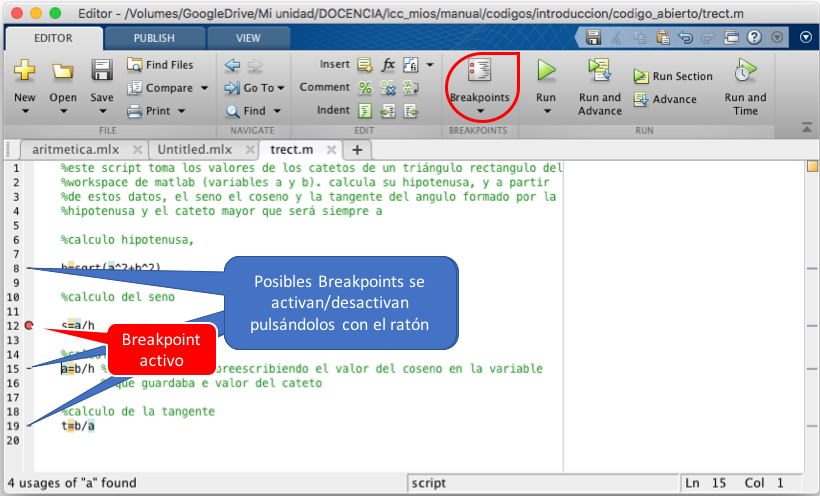
\includegraphics[width=14cm]{depu1.png}
\bicaption{Breakpoint activo señalado con una flecha azul, y menú desplegable \emph{debug}}{Active Breackpoint pointed by a blue arrow and \emph{debug} drop-down menu}
\label{fig:depu1}
\end{figure}

\begin{paracol}{2}
Si una vez señalado el \emph{breakpoint},  entramos en el modo de depuración, Pulsando el primero de los botones azules en la parte superior del editor de textos (ver figura \ref{fig:depu2}),
Spyder nos indica que ha detenido la ejecución del programa en la línea marcada por el \emph{breakpoint} (línea 35 en el ejemplo). Además, en el terminal de Ipython nos indica también que ha entrado en el modo de depuración,
\switchcolumn
Suppose after activating the \emph{breakpoint}, we start the debugging mode by pressing the first of the blue buttons located on top of the text editor (see figure \ref{fig:depu2}). In that case, Spyder shows us that it has stopped the program run at the line marked by the \emph{breakpoint} red dot (line 35 in the example). Besides, the Ipython console also shows that it has come into debugging mode.
\end{paracol}
\begin{minted}{python}
IPdb [1]: !continue
> c:\users\abierto\documents\borrar\eq_seg_grado.py(35)<module>()
     33 #here we add a 'how to use' example that's not part of the function
     34 
2--> 35 solplus, solminus = soleq2(2, 3, 1)
     36 
     37 #comprobacion


IPdb [2]: 
\end{minted}
\begin{figure}
\centering
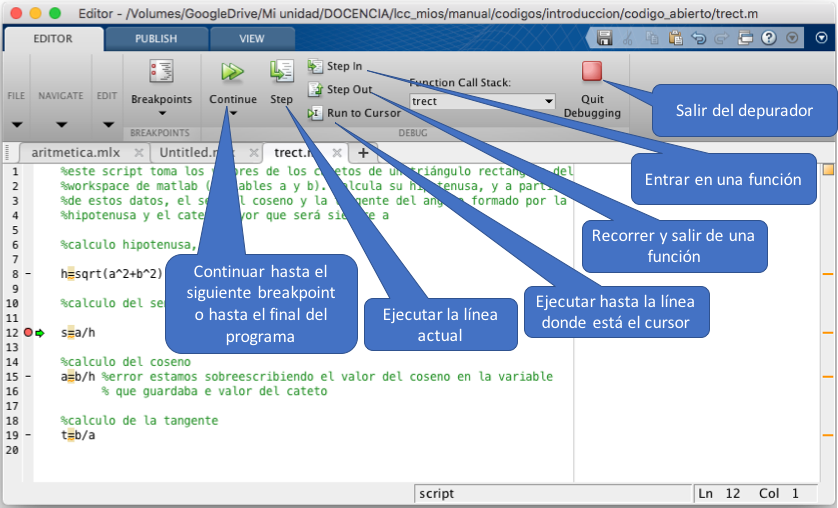
\includegraphics[width=14cm]{depu2.png}
\bicaption{Parada de programa en un breakpoint y herramientas de depuración}{program stop on a breakpoint and debugging tools}
\label{fig:depu2}
\end{figure}

\begin{paracol}{2}
A partir de aquí Spyder pone a nuestra disposición las herramientas de depuración, la figura \ref{fig:depu2} muestra la línea en que se ha parado la ejecución del programa, (señalada con una flecha verde), y algunas de estas herramientas. Se trata del mismo módulo de ejemplos anteriores, en el que hemos introducido un pequeño error en la línea $28$.  Básicamente, Spyder nos da la posibilidad de ejecutar el código línea a línea, de entrar e ir línea a línea en las funciones que llama nuestro programa, o de de continuar la ejecución hasta el final del programa o hasta el siguiente \emph{breakpoint}.

Si pulsamos el botón ``ejecutar línea actual'' Spyder ejecutará la línea de programa señalada con la flecha verde y se parará en la línea siguiente. En cada paso, podemos ver el valor que toman las variables, pidiendo su valor directamente en el terminal de Ipython. En el ejmplo de la figura, el breakpoint está situado en la línea $35$ que corresponde a la llamada a la función \mintinline{python}{soleq}. Si volvemos a pulsar el `ejecutar la línea actual'', el depurador ejecutará la función y saltará directamente a la linea $39$. Si queremos que recorra paso a paso el código correspondiente a la función, empleamos el el botón ``entrar en la función de la línea actual''. El uso del resto de las opciones del depurador el bastante evidente (ver figura \ref{fig:depu2}). Si entramos en la función, ejecutamos su código línea a línea y vamos comprobando el resultado que deberían dar, comprobaremos que la línea $28$ no da un resultado correcto y estaremos en condiciones de repasar su código y descubrir el error. ¿Cúal es?.
\switchcolumn
Now, we can access Spyder debugger's tools. Figure \ref{fig:depu2} shows the line where the program execution has been stopped. (Marked with a green arrow) and some of these tools. It is the same modules used in previous examples, but we have added a small error in line $28$ this time. Spyder allows us to run the program line by line, get into the function our program calls to and cover them line by line, or continue the program execution till the next breakpoint or to the program end. 

If we select the button ``Run the current line,'' the program will execute the code line marked with the green arrow and stop in the following line. In each step, we can check the values the variables so far defined take by asking for them at the Ipython terminal. In the example shown in the figure, the breakpoint is located in line $35$, where the program calls to \mintinline{python}{soleq} function. If we push the button ``Run the current line'' again, the debugger will execute the function and jump to line $39$. If we want to cover line by line the function \mintinline{python}{soleq}, then we may push the button ``Get into the function of the current line''. The performance of the remaining debugger tools is easy to understand, looking at figure \ref{fig:depu2}. If we get into the function \mintinline{python}{soleq} and execute its code line by line, checking their results, we will realise that there is a bug in line $28$ because the result cast by this line is wrong. So we would be ready to review its code and discover the error. Can you find it?   
\switchcolumn
\section{Control de Flujo}\index{Flujo} \index{Control de flujo}
En la sección anterior, se introdujo el modo de escribir programas en Python mediante el uso de 	\emph{scripts} y funciones. En todos los casos vistos, la ejecución del programa empezaba por la primera línea del programa, y continuaba, por orden, línea tras línea hasta alcanzar el final del programa. Se trata de programas en los que el \emph{flujo} es lineal, porque los resultados de cada línea de programa se van obteniendo regularmente uno detrás de otro. 

Hay ocasiones en las que, por diferentes razones que expondremos a continuación, puede interesarnos alterar el orden en que se ejecutan las sentencias de un programa, bien repitiendo una parte de los cálculos un determinado número de veces o bien ejecutando unas partes de código u otras en función de que se satisfagan unas determinadas condiciones.

El control del orden en que se ejecutan las sentencias de un programa es lo que se conoce con el nombre de \emph{control de flujo}. Veremos dos tipos principales de control de flujo: El flujo condicional y los bucles.
\subsection{Flujo condicional.}\index{Flujo!Condicional}
Empezaremos con un ejemplo sencillo de cómo y para qué condicionar el flujo de un programa. Supongamos que queremos construir un programa que reciba como variable de entrada un número cualquiera y nos muestra un mensaje por pantalla si el número es par.

Para ello, podríamos hacer uso del operador, \emph{resto de la división entera}, \mintinline{python}{%}. Si el resto de la división entre dos del número suministrado a la función es cero, se trata de un número par; si no, es un número impar. Podríamos hacer uso de operadores relacionales, en particular de \mintinline{python}{==} para comprobar si el resto de la división entre dos es cero. Por último necesitaríamos algún mecanismo que permitiera al programa escribir un mensaje solo cuando el número introducido sea par.

\paragraph{if - elif - else.} El mecanismo que necesitamos nos lo suministra la estructura \mintinline{python}{if} de Python. Veamos en primer lugar el código del ejemplo del que venimos hablando,
\switchcolumn
\section{Flow control} \index[eng]{flow} \index[eng]{flow control}
In the previous section, we introduced how to write Python programs using scripts and functions. In all the examples shown, the programs ran from the first line and went on, in an orderly manner, line after line, until the program ended. These programs follow a linear \emph{flow} because the results of each line are obtained sequentially, one after another.

Many times, in situations we will describe later, we would like to modify the order in which the program sentences are executed. Sometimes, we need to repeat a block of code several times, while other times, we want a chunk of code to be executed only when a predefined condition is fulfilled. 

The control of the order a program follows when executing its sentences is known as \emph{flow control}. We will describe two main kinds of flow control: Conditional flow and loops.
\subsection{Conditional flow.} \index[eng]{flow!Conditional}
We begin with a simple example of how and why conditioning the flow. Suppose we want to make a program that takes a number as input and shows us a message if the number is even. 
\end{paracol}

\inputminted[
frame=lines,
framesep=2mm,
baselinestretch=1.2,
%bgcolor=LightGray,
label=Example\_import.py,
fontsize=\footnotesize,
linenos
]{python}{./codigos/introduccion/codigo_abierto/numero_par.py}

\begin{paracol}{2}
El script genera una función \mintinline{python}{par(a)}. En la línea $17$ aparece definida la entrada a una bloque \mintinline{python}{if}. Empieza con la palabra clave \emph{if} que va siempre seguida de una expresión que da un resultado lógico: verdadero ($1$) o falso ($0$). Esta expresión puede ser cualquier combinación válida de expresiones relacionales o lógicas.  

En nuestro caso comparamos el resto de la división del número introducido entre 2 con cero. La entrada del bloque constituye una condición, y termina siembre con el símbolo ``dos puntos'' (:). El cuerpo del bloque mintinline{python}{if} lo constituyan las líneas posteriores a la línea de entrada, que deben estar sangradas. Estas líneas solo se ejecutan si se cumple la condición de la entrada del bloque \mintinline{python}{if}. En nuestro caso, el cuerpo lo constituyen las líneas $18$ y $19$. Por último, la línea $20$ corresponde al comando \mintinline{python}{return()} que está alineado con las líneas de código de la función, no con las de bloque mintinline{python}{if}. Por tanto, en nuestro ejemplo, si el número introducido no es par, la función se saltará todas las líneas del cuerpo del bloque \mintinline{python}{if} e irá directamente a la línea $20$.
En las líneas siguientes se muestra un ejemplo del funcionamiento de la función \mintinline{python}{par}. Para probarla hemos importado directamente la función en el terminal de Ipython, y luego la hemos llamado dándole como variable de entrada primero el  número $3$ y luego el número $8$ en el primer caso no se cumple la condición impuesta, ya que el número no es par, por tanto la función se salta todo el bloque condicional, y ejecutamente directamente el comando \mintinline{python}{return()}. Como no hemos pedido que devuelva nada, la función no devuelve nada. En el segundo caso, el número es par y por tanto si se cumple la condición necesaria para ejecutar el bloque \mintinline{python}{if}. Como resultado, la función imprime en el terminal de Ipython el mensaje indicado. Una vez que acaba la eejecución del bloque condicional, ejecuta la función \mintinline{python}{return()} igual que en el caso anterior.

\end{paracol}

\begin{center}
    \begin{minipage}{.4\textwidth}
\begin{minted}{python}
In [2]: from numero_par import par

In [3]: par(3)
Out[3]: ()
In [4]: par(8)
8  es un numero par
8 is an even number
Out[4]: ()
\end{minted}
\end{minipage}
\end{center}
======================THE FRONTIER=====================
 






% \begin{lstlisting}
% function espar(x)
% % Este programa recibe un numero entero como variable de entrada. y muestra
% % por pantalla un mensaje indicando si el numero recibido es par o impar.

% % Calculamos el resto de la division por dos
% resto=rem(x,2);

% % Empleamos una estructura if - else -end para decidir que mensaje mostrar

% if resto==0
%     % si el resto es cero el número es par
%     disp('el número es par')
% end
% \end{lstlisting}

 



En nuestro ejemplo, se emplea una expresión relacional sencilla \texttt{resto==0}. Si se cumple, el programa ejecutará la siguiente línea de programa, escribiendo en la ventana de comandos la frase ``el número es par"  si no se cumple el programa se la salta, llega hasta el \texttt{end}, y no escribe nada por pantalla. 

Acabamos de ver la estructura condicional \texttt{if} más sencilla posible. Podríamos complicarla un poco pidiendo que también nos saque un mensaje por pantalla cuando el número sea impar. Esto supone incluir en nuestro programa una disyuntiva; si es par el programa debe hacer una cosa y si no, debe hacer otra. Para incluir este tipo de disyuntivas en una estructura \texttt{if}, se emplea la palabra clave \texttt{else}. Veamos nuestro ejemplo modificado,
% \begin{lstlisting}
% function espar(x)
% % Este programa recibe un numero entero como variable de entrada. y muestra
% % por pantalla un mensaje indicando si el numero recibido es par o impar.

% % Calculamos el resto de la division por dos
% resto=rem(x,2);

% % Empleamos una estructura if - else -end para decidir que mensaje mostrar

% if resto==0
%     % si el resto es cero el número es par
%     disp('el número es par')
% else
%     % si el resto no es cero el número es impar
%     disp('el número es impar')
% end 
% \end{lstlisting}

La palabra clave \texttt{else} marca ahora la disyuntiva, si el número es par, el programa ejecuta las líneas de código entre el \texttt{if} y el \texttt{else}, si el número no es par ejecutará las líneas entre el \texttt{else} y el \texttt{end}.

La estructura \texttt{if} admite todavía ampliar el número de posibilidades de elección mediante la palabra clave \texttt{elseif}. Al igual que  con \texttt{if}, \texttt{elseif} va seguido de una expresión lógica que establece una condición, si se cumple se ejecutará el código de las líneas siguientes, si no se cumple, el programa saltará a la siguiente línea que contenga una palabra clave: otro \texttt{elseif}, un \texttt{else} o directamente el \texttt{end} que marca el final de la parte de código condicional. Para ver cómo funciona, vamos a modificar nuestro ejemplo anterior, para que, si el número introducido no es divisible por dos, compruebe si es divisible por tres,

% \begin{lstlisting}
% function divis(x)
% % Este programa recibe un numero entero como variable de entrada. y muestra
% % por pantalla un mensaje indicando si el numero recibido es par. Si no 
% % es par, comprueba si es divisible por 3 y si lo es muestra un mensaje   
% % por pantalla indicandolo. Si no es par ni divisible por tres muestra un
% % mensaje diciendo que no es par ni disible por tres. 



% % Empleamos una estructura if-elseif-else-end para decidir que mensaje mostrar

% if rem(x,2)==0
%     % si el resto es cero el número es par
%     disp('el número es par')
% elseif rem(x,3)==0
%     % El número es divisible por tres
%     disp('el número es divisible por 3')
% else
%     % el numero no es par ni divisible por tres
%     disp('el número no es par ni divisible por 3')
% end
% \end{lstlisting}

Si llamamos ahora a la función dando como valor de entrada un número par, Ejecutará el código situado debajo del \texttt{if} y antes del \texttt{elseif} y se saltará todo lo demás hasta llegar al \texttt{end}. Si el número introducido no es par, pero es divisible por tres, se saltará el código situado por debajo del \texttt{if}, ejecutará el código contenido debajo del \texttt{elseif} hasta el \texttt{else} y saltará el resto del código hasta llegar al \texttt{end}. Por último si el número no es par ni divisible por tres, solo ejecutará el código situado por debajo del \texttt{else}.

Un aspecto que debemos resaltar, es que el programa ejecutará el código correspondiente a la primera condición que se cumpla, y se saltará el resto hasta llegar al \texttt{end}. Así por ejemplo, si en nuestro ejemplo introducimos el número $6$, el programa nos mostrará el mensaje ``el número es par", puesto que ésta es la primera condición que se cumple, pero nunca nos mostrará el mensaje ``el número es divisible por 3". Porque una vez comprobada y cumplida la primera condición (ser par) el programa salta directamente al \texttt{end} final de la estructura, sin comprobar nada más. La figura \ref{fig:if} muestra el esquema completo de una estructura \texttt{if}. Los términos entre paréntesis pueden estar o no presentes en una implementación concreta.

\begin{figure}[h]
\centering
\begin{tikzpicture}
%\usetikzlibrary{shapes.multipart}
\path (5,0) node(a) [rectangle split,rectangle split parts =2,draw=blue,top color=white,bottom color=blue!15, very thick,align=left,rounded corners]{Estructura if-elseif-else-end
\nodepart{two}

if condición\\
\ \ \ ... código\\
\ \ \ ...\\
(elseif condición)\\
\ \ \ ... código\\
\ \ \ ...\\
(elseif condición)\\
\ \ \ ... código\\
\ \ \ ...\\
.\\
(puede haber tantos bloques elseif como se necesiten)\\
.\\
(else)\\
\ \ \ ... código\\
\ \ \ ...\\
end};		
\end{tikzpicture}
\caption{Esquema general de la estructura de flujo condicional \texttt{if} los términos escritos entre paréntesis son opcionales.}
\label{fig:if}
\end{figure} 

\paragraph{Estructuras if anidadas.}\index{Anidación! If anidado} 
En el ejemplo anterior, hemos visto cómo, si el número introducido en la función era par y además divisible por tres, el programa nunca nos informaría de esta segunda propiedad, debido al carácter excluyente de la estructura \emph{if}. Una manera de resolver este problema, es mediante el uso de estructuras \texttt{if} anidadas. La idea es muy sencilla, se construye una estructura \texttt{if} para comprobar una determinada condición, si esta se cumple, dentro de su código se construye otra estructura if para comprobar una segunda condición, y así sucesivamente, todas las veces que sea necesario. Si modificamos nuestro ejemplo anterior, incluyendo un \texttt{if} anidado,

% \begin{lstlisting}
% function divis23(x)
% % Este programa recibe un numero entero como variable de entrada. y 
% % muestra por pantalla un mensaje indicando si el numero recibido es par. 
% % si el numero es par y divisible entre tres,
% % si es divisible entre tres  
% % Si no es par ni divisible por tres 



% % Empleamos una estructura if - else -end 
% % y un if anidado para decidir que mensaje mostrar

% if rem(x,2)==0
%     % si el resto es cero el número es par
%     % comprobamos con un if anidado si además es divisible entre tres
%     if rem(x,3)==0
%         disp('el número es par y divisible entre tres')
%     else
%         disp('el número es par')
%     end
% elseif rem(x,3)==0
%     % El número es divisble entre tres
%     disp('el número es divisible entre 3')
% else
%     % el numero no es par ni divisible entre tres
%     disp('el número no es par ni divisible entre tres')
% end
% \end{lstlisting}

\paragraph{Switch-case-otherwise.} \index{Flujo! Switch-case}Se trata de otra estructura que permite también ejecutar una parte u otra de código de acuerdo con unas codiciones preestablecida. Estas condiciones se presentan en forma de \emph{casos}, el programa comprueba al llegar a la estructura \texttt{switch} de qué caso se trata y ejecuta el código correspondiente. La figura \ref{fig:switch} muestra la forma general que toma una estructura \texttt{switch}.

La estructura \texttt{switch}, compara el valor contenido en la variable de entrada a la estructura con las expresiones contenidas en los casos, ejecutando el primer caso para el que coincidan. Si no encuentra ninguno, ejecuta entonces el código contenido debajo de la sentencia \texttt{otherwise}.

Veamos un ejemplo muy sencillo,

% \begin{lstlisting}
% function signo(x)
% % este programa emplea una estructura switch para informarnos del signo de
% % un número.

% % NOTA EL PROGRAMA NO COMPRUEBA QUE LA VARIABLE DE ENTRADA X SEA UN NUMERO,
% % SI ES UN VECTOR O UNA MATRIZ EL RESULTADO NO TIENE SENTIDO
  
% s=sign(x); % obtnemos el signo del número mediante la función sign

% % construimos la estructura switch,

% switch s
%     case 1
%         disp('el número es positivo')
%     case -1
%         disp('el número es negativo')
%     otherwise
%         disp('el número es cero')
% end

% \end{lstlisting}

\begin{figure}[h]
\centering
\begin{tikzpicture}
%\usetikzlibrary{shapes.multipart}
\path (5,0) node(a) [rectangle split,rectangle split parts =2,draw=green,top color=white,bottom color=green!20, very thick,align=left,rounded corners]{Estructura switch-case-otherwise
\nodepart{two}
switch variable\\
\ \ \ case expresión\\
\ \ \ \ \ ... código\\
\ \ \ case expresión\\
\ \ \ \ \ ... código\\
\ \ \ .\\
Puede haber tantos bloques \emph{case} como se necesiten\\
\ \ \ .\\
\ \ \ otherwise\\
\ \ \ \ \ ... código\\
end};		
\end{tikzpicture}
\caption{Esquema general de la estructura switch-case-otherwise}
\label{fig:switch}
\end{figure}

La función del ejemplo emplea a su vez la función de Matlab \texttt{sign} para obtener el signo ($1$, $-1$, $0$) del número introducido. Guarda el resultado de esta operación en la variable \texttt{s}, que será precisamente la variable de entrada a la estructura \texttt{switch}. Los casos se limitan a chequear los posibles valores de la variable y enviar a la ventana de comandos el mensaje correspondiente.
 
\subsection{Bucles}\index{Flujo!Bucles}\index{Bucles}
En ocasiones, es preciso repetir una operación un número determinado de veces o hasta que se cumple una cierta condición. Los lenguajes de alto nivel poseen estructuras específicas, para repetir la ejecución de un trozo de programa las veces que sea necesario. Cada repetición recibe el nombre de iteración. Estas estructuras reciben el nombre genérico de bucles. Vamos a ver dos tipos: los bucles \texttt{for} y los bucles \texttt{while}.

\paragraph{Bucles for.} \index{Flujo! Bucle for}\index{Bucles! Bucle for}Un bucle \texttt{for} repite las sentencias contenidas en el bucle un determinado número de veces, es decir realiza un número fijo de iteraciones. La estructura general de un bucle \texttt{for} se muestra en la figura, \ref{fig:for}

\begin{figure}[h]
\centering
\begin{tikzpicture}
%\usetikzlibrary{shapes.multipart}
\path (5,0) node(a) [rectangle split,rectangle split parts =2,draw=orange,top color=white,bottom color=orange!30, very thick,align=left,rounded corners]{Estructura de un bucle for
\nodepart{two}

for indice=[vector de valores]\\
\ \ \ ... código\\
(condición: Break)\\
\ \ \ ...\\
(condicición: Continue)\\
\ \ \ ... código\\

end};		
\end{tikzpicture}
\caption{Esquema general de la estructura de un bucle \texttt{for} los términos escritos entre paréntesis son opcionales.}
\label{fig:for}
\end{figure} 
 
El bucle empieza con la palabra clave for, seguida de una variable a la que hemos dado el nombre genérico de índice. Esta variable irá tomando sucesivamente los valores de los elementos contenidos en el [vector de valores]. El código contenido en el bucle, desde la línea siguiente al \texttt{for} hasta el \texttt{end} se ejecutará tantas veces como valores tenga el vector de valores. Antes de hablar de las sentencias \texttt{break} y \texttt{continue}, veamos alguno ejemplos.
% \begin{lstlisting}
% function y=demofor(x)
% % este programa emplea un bucle for sencillo para ir mostrando uno 
% % a uno los elementos del vector de entrada x por pantalla. además  
% % los suma y guarda el resultado total en el vector y,

% y=0; % iniciamos la suma a cero

% for i=x
%     disp(i)
%     y=y+i;
% end
% \end{lstlisting}

Si ejecutamos el programa, usando como entrada el vector \texttt{d=[1 9 4 18]},

\begin{verbatim}
>> d=[1 9 4 18]

d =

     1     9     4    18

>> suma=demofor(d)
     1

     9

     4

    18


suma =

    32
\end{verbatim}

Una vez que el programa llega al bucle \texttt{for}, iguala la variable \texttt{i} al primer valor contenido en el vector de entrada, lo muestra por pantalla y añade su valor a la variable de salida. cuando llega al \texttt{end} del bucle for comprueba que todavía quedan valores del vector de entrada por recorrer, así que vuelve al principio del \texttt{for}, igual la variable \texttt{i} al segundo valor del vector de entrada, suma dicho valor a la variable de salida, llega al \texttt{end} y así sucesivamente hasta que haya recorrido todos los valores del vector de entrada.

El uso más habitual de los bucles, es para recorrer elementos de un vector o de una matriz. por esta razón, lo más frecuente es que no se de explícitamente el vector cuyos elementos debe recorrer el índice del \texttt{for}, sino que se construya empleado el operador \texttt{:},
\begin{verbatim}
for indice=principio:incremento:final
\end{verbatim}

Veamos un ejemplo sencillo para obtener el vector suma de dos vectores,
% \begin{lstlisting}
% function s=sumafor(x,y)
% % este programa emplea un bucle for sencillo para sumar dos vectores
% % primero comprueba si son del mismo tamaño. Si no lo son da un mensaje 
% % de aviso

% l1=length(x);
% l2=length(y);
% if l1==l2
%     % construimos un vector de ceros del mismo tamaño que x e y paraa
%     % guardar el resultado de la suma,
%     s=zeros(size(x));
%     % si son iguales los suma elemento a elemento usando un bucle for
%     for i=1:l1
%         s(i)=x(i)+y(i);
%     end
% else
%     disp('los vectores son de distinto tamaño')
% end
% \end{lstlisting}

En la figura \ref{fig:for}, aparecen dos sentencias opcionales, \texttt{break} y \texttt{continue}.

La sentencia \texttt{break}, permite terminar el bucle \texttt{for} antes de que haya terminado de realizar todas las ejecuciones previstas. La sentencia break va siempre incluida dentro de una condición que, si se cumple interrumpe la ejecución del bucle. Por ejemplo, podemos emplear un bucle \texttt{for} y una sentencia \texttt{break}, para buscar la primera vez que un determinado número aparece en un vector,

% \begin{lstlisting}
% function posicion=buscanum(x,n)
% % este programa emplea un bucle for y un break para buscar en el  
% % vector x, la primera vez que aparece el número n

% % obtenemos la longitud del vector
% l1=length(x);
% % iniciamos la variable posicion a un valor absurdo
% posicion=-1;
% for i=1:l1
%     if x(i)==n
%         posicion=i:
%         break
%     end
% end
% if posicion==-1
%     disp('el numero pedido no se encuentra en el vector x') 
% end
% \end{lstlisting} 

El programa toma como variables de entrada un vector y el número que debe buscar dentro del vector. Construye un bucle \texttt{for}, con el mismo número de iteraciones que el tamaño del vector. El bucle va comparando los elementos del vector con el número pedido. Cuando encuentra un elemento igual, se ejecuta el código de la estructura if contenida en el bucle; la variable posición toma el valor del índice \texttt{i} del bucle y la sentencia \texttt{break} interrumpe la ejecución del bucle, saltando al final del mismo. Por último, se ha añadido una condición al terminar el bucle, para el caso de que se hayan recorrido todos los elementos del vector sin encontrar el número pedido.

La sentencia \texttt{continue}, se emplea para hacer que una determinada iteración interrumpa su ejecución y salte directamente al comienzo de la siguiente iteración. Debe ir, como en el caso de la sentencia \texttt{break}, incluida en una estructura condicional. Veamos un ejemplo para entender como funciona. Se trata de un programa que admite como entrada un vector de cualquier longitud y devuelve como salida otro vector que contiene solo los números pares contenidos en el vector de entrada,

% \begin{lstlisting}
% function pares=buscapar(x)
% % este programa emplea un bucle for y un continue para construir un 
% % vector de salida con los numeros pares contenidos en el vector de entrada.

% % obtenemos la longitud del vector
% l1=length(x);
% % iniciamos el vector de salida a un vector vacío,
% pares=[];
% for i=1:l1
%     if rem(x(i),2)~=0
%         continue
%     end
%     pares=[pares x(i)];
% end
% \end{lstlisting}

El funcionamiento es muy sencillo, en cada iteración la sentencia \texttt{if} comprueba si el número es par. Si no lo es, entra en el código de la estructura \texttt{if}, ejecuta la sentencia \texttt{continue}, y se salta el resto del código del bucle, volviendo directamente a empezar la siguiente iteración.

\paragraph{bucles for anidados.} \index{Anidación!For anidado}Los bucles \texttt{for} pueden anidarse unos dentro de otros de modo análogo a como se hace con las estructuras \texttt{if}. Veamos un ejemplo de uso, muy común; calcular la suma de dos matrices,

% \begin{lstlisting}
% function s=suma_mat(x,y)
% % este programa emplea dos bucles for anidados para obtener la suma de 
% % dos matrices.

% % obtenemos el tamaño de las matrices,
% t1=size(x);
% t2=size(y);
% if t1(1)==t2(1)&& t1(2)==t2(2)
%     % si las matrices tienen el mismo tamaño pueden sumarse...
%     % construimos una matriz de dicho tamaño para guardar el 
%     % resultado de la suma
%     s=zeros(size(x));
%     % construimos un bucle que recorre las filas de ambas matrices
%     for i=1:t1(1)
%         % y dentro, anidamos un bucle que recorre las columnas
%         for j=1:t1(2)
%             % Empleando ambos índices para ir sumando los elementos 
%             % de las dos matrices,
%             s(i,j)=x(i,j)+y(i,j);
%         end
%     end
% else
%     % si no tienen el mismo tamaño no se pueden sumar...
%     disp('las matrices no son del mismo tamaño')
% end
% \end{lstlisting} 

Es interesante observar en este ejemplo el funcionamiento de los dos bucles anidados. Cada interación del bucle exterior, avanza una fila, en el recorrido de las matrices, cada iteración del bucle interior recorre todos los elementos de la fila indicada por el bucle exterior.

\paragraph{bucle while.} \index{Flujo! Bucle while}\index{Bucles! Bucle while} Este bucle tiene la misma finalidad que un bucle \texttt{for}, repetir un trozo de código un determinado número de veces. Lo que cambia, es el mecanismo que determina cuantas iteraciones realizará el bucle. En el caso de un bucle \texttt{while} las iteraciones se repiten un número indefinido de veces mientras se cumpla una determinada condición impuesta al principio del bucle. La figura \ref{fig:while} muestra la estructura general de un bucle while.

\begin{figure}[h]
\centering
\begin{tikzpicture}
%\usetikzlibrary{shapes.multipart}
\path (5,0) node(a) [rectangle split,rectangle split parts =2,draw=yellow,top color=white,bottom color=yellow!40, very thick,align=left,rounded corners]{Estructura de un bucle while
\nodepart{two}

while condición\\
\ \ \ ... código\\
(condición: Break)\\
\ \ \ ...\\
(condicición: Continue)\\
\ \ \ ... código\\
end};		
\end{tikzpicture}
\caption{Esquema general de la estructura de un bucle \texttt{while} los términos escritos entre paréntesis son opcionales.}
\label{fig:while}
\end{figure}

Veamos un ejemplo sencillo. 

% \begin{lstlisting}
% function n=potencia(x,max)
% % este programa emplea un bucle while para calcular la potencia a 
% % la que hay que elevar un número x para que el resultado sea mayor 
% % que otro determinado número max
% % un número.

% % NOTA EL PROGRAMA NO COMPRUEBA QUE LA VARIABLE DE ENTRADA X SEA UN NUMERO,
% % Si ES UN VECTOR O UNA MATRIZ EL RESULTADO NO TIENE SENTIDO
  
% pot=1;
% n=0;
% while pot<max % mientras la potencia calculada sea menor que max
%     n=n+1;
%     pot=x^n;
% end
% \end{lstlisting}

El programa emplea un bucle \texttt{while} para calcular el exponente mínimo al que hay que elevar un número para que rebase una determinada cantidad. El bucle while se ejecuta mientras la potencia calculada sea menor que la variable \texttt{max}; una vez que la potencia rebasa dicho valor el bucle deja de ejecutarse. Un aspecto muy importante del bucle \texttt{while} es que al programarlo hay que asegurarse de que dentro del bucle existe la posibilidad de cambiar la condición de entrada. Si no, el programa no podrá terminar nunca el bucle\footnote{Cuando se produce esta situación por un error en el diseño del programa, el bucle se puede parar pulsando a la vez las teclas ctrl+c}.

Las sentencias \texttt{break} y \texttt{continue} son idénticas a las descritas en el caso de los bucles \texttt{for}, por lo que no insistiremos más sobre el asunto.

\paragraph{Bucles while anidados.} \index{Anidación! While anidado} Del mismo modo que se anidan los bucles \texttt{for}, es posible anidar bucles \texttt{while}. Como un ejemplo, vamos a reproducir el programa desarrollado antes para sumar dos matrices, empleando ahora bucles \texttt{while}.

% \begin{lstlisting}
% function s=suma_while(x,y)
% % este programa emplea dos bucles while anidados para obtener la 
% % suma de dos matrices.

% % obtenemos el tamaño de las matrices,
% t1=size(x);
% t2=size(y);
% if t1(1)==t2(1)&& t1(2)==t2(2)
%     % si las matrices tienen el mismo tamaño pueden sumarse...
%     % construimos una matriz de dicho tamaño para guardar el 
%     % resultado de la suma
%     s=zeros(size(x));
%     % construimos un bucle que recorre las filas de ambas matrices
%     i=1; % inicimos un contador para las filas
%     while i<=t1(1)
%         % y dentro, anidamos un bucle que recorre las columnas
%         j=1; % iniciamos un contador para las columnas
%         while j<=t1(2)
%             % Empleando ambos índices para ir sumando los elementos 
%             % de las dos matrices,
%             s(i,j)=x(i,j)+y(i,j);
%             j=j+1; % vamos incrementando el indice de columnas
%         end
%         i=i+1; % vamos incrementando el indice de filas
%     end
% else
%     % si no tienen el mismo tamaño no se pueden sumar...
%     disp('las matrices no son del mismo tamaño')
% end
% \end{lstlisting}

El ejemplo, es más complicado de programar y menos eficiente que si usáramos bucles \texttt{for}. La razón de incluirlo es puramente ilustrativa. En general, un bucle \texttt{while} debe utilizarse solo cuando el número de iteraciones que se precisa realizar no es fijo, sino que depende de alguna condición propia de los resultados que se van obteniendo a medida que se van realizando iteraciones.

\subsection{Funciones recursivas.} \index{Funciones! Recursivas}
Una función recursiva es una función que se llama a sí misma. Hemos esperado hasta aquí para hablar de ellas porque, de alguna manera, se comportan como un bucle y necesitan una condición de salida para dejar de llamarse a sí mismas y terminar su ejecución. En general, son delicadas de manejar y tienden a consumir mucha memoria ya que cada vez que la función se llama a sí misma necesita crear un nuevo espacio de memoria independiente. Veamos un ejemplo de función recurrente que permite obtener el término enésimo de la sucesión de Fibonacci  
\begin{align*}
f_0=0, f_1=1, f_2=1, f_3=2, f_4=3, f_5=5, f_6=8, \cdots f_i=f_{i-1}+f_{i-2} \cdots 
\end{align*}

La sucesión empieza con los términos $0$ y $1$ y a partir de ahí cada término es la suma de los dos anteriores. Podemos convertir directamente esta definición en código,

%\lstinputlisting{../codigo/matlab/introduccion/fibonacci.m}

Si n es menor que dos, la función da como valor el término correspondiente (1 o 0). Si n es mayor que dos, vuelve a llamarse a si misma con entrada \texttt{n-1} y \texttt{n-2}, para calcular el valor enésimo de la sucesión a partir de la suma de los dos anteriores, la función se irá llamando a sí misma hasta  llegar a $n<2$. A partir de ahí ira devolviendo los valores obtenidos en cada llamada hasta obtener el enésimo término.

\subsection{Algoritmos y diagramas de flujo.} \index{Flujo! Diagrama de Flujo}
Un algoritmo es, en la definición de la Real Academia: 
\begin{quotation}
Un conjunto ordenado y finito de operaciones que permite hallar la solución de un problema.
\end{quotation}

La palabra algoritmo ha llegado hasta nosotros transcrita del nombre del matemático árabe \emph{Al-Juarismi} (circa 780-850 dc). En programación los algoritmos son importantes, porque suponen un paso previo a la creación de un programa.

Habitualmente, partimos de un problema para el que tenemos un enunciado concreto. Por ejemplo: obtener los $n$ primeros números primos. 

El siguiente paso, sería pensar y definir un algoritmo que permita resolver nuestro problema, es importante caer en la cuenta de que un mismo problema puede resolverse, en muchos casos, por distintos caminos. Por tanto es posible diseñar distintos algoritmos para resolver un mismo problema. Un posible algoritmo para el problema de los números primos sería el siguiente,

\begin{itemize}
\item Considerar 2 como el primer números primo. (un número primo es aquel que solo es divisible por si mismo o por uno.)
\item Recorrer todos los números impares desde 3 hasta que se complete el número $n$ de números primos solicitados.
\item Para cada número, probar a dividirlo por todos los primos obtenidos hasta ese momento. Si no es divisible por ninguno, el número es primo y se guarda, si es divisible por alguno de ellos, se interrumpe el proceso y se prueba con el siguiente.
\end{itemize}

En ocasiones, facilita la comprensión de un algoritmo representarlo gráficamente mediante un diagrama de flujo. Los diagramas de flujo emplean símbolos bien definidos para representar los distintos paso de un algoritmo y flechas para indicar la relación entre ellos; la relación en la que la información \emph{fluye} de un paso del algoritmo a otro.

No hay una norma rígida para realizar un diagrama de flujo, el grado de detalle con que se describe el algoritmo va en función de las necesidades del programador, o de los destinatarios a quienes va dirigido el diagrama. La idea fundamental es que facilite la comprensión del algoritmo. Se utilizan diversos símbolos para indicar, procedimientos, condiciones, almacenamiento de resultados, etc. La figura \ref{fig:flujo} muestra los tres símbolos más empleados.

\begin{figure}[h]
\centering
\begin{tikzpicture}
%\usetikzlibrary{shapes.geometric}
\path (5,0) node(a) [ellipse,draw=blue, very thick,align=center]{Inicio y fin del algoritmo}
(5,-2) node(b)[rectangle,draw=blue, thick,rounded corners,align=center]{procedimentos}
(5,-4) node(c)[diamond,aspect=3,draw=red,thick]{flujo condicional};
\end{tikzpicture}
\caption{Símbolos empleados en diagramas de flujo}
\label{fig:flujo}
\end{figure}

Para indicar el inicio y el fin de un algoritmo se emplea como símbolo una elipse. Para indicar un procedimiento concreto, como por ejemplo realizar un cálculo, asignar un valor a una variable, etc, se emplea como símbolo un rectángulo. Por último se emplea un rombo como símbolo, para representar una condición.

Los símbolos se relacionan mediante flechas que indican el sentido en que se ejecuta el algoritmo. los rombos suelen tener dos flechas de salida marcadas con las palabras ``si'' y ``no'', para indicar por donde sigue el flujo de información dependiendo de si la condición representada se cumple o no.

Por último un bucle se representa habitualmente mediante una flecha que devuelve el flujo a un símbolo ya recorrido anteriormente. 

\begin{figure}
\centering
\begin{tikzpicture}
%\usetikzlibrary{shapes.geometric}
\path (6,0) node(a) [ellipse,draw=blue, very thick,align=center]{inicio}
(6,-1.5) node(b)[rectangle,draw=blue, thick,rounded corners,align=center]{Introducir cuantos\\
números primos se desea obtener ($n$)}
(6,-3) node(c)[rectangle,draw=blue, thick,rounded corners,align=center]{guardar el número $2$\\
como primer número primo}
(6,-5) node(d)[diamond,aspect=3,draw=red,align=center,thick]{¿Se ha alcanzado\\ la cifra pedida de primos?}
(11,-5) node(e)[ellipse,draw=blue,align=center,very thick]{fin}
(6,-7) node(f)[rectangle,draw=blue, thick,rounded corners,align=center]{tomar el siguiente número impar}
(6,-8.3) node(g)[rectangle,draw=blue, thick,rounded corners,align=center]{tomar el primer numero primo\\ de los ya encotrados}
(6,-10.5) node(h)[diamond,aspect=3,draw=red,align=center,thick]{¿Es divisible el impar entre el primo?}
(6,-13.5) node(i)[diamond,aspect=3,draw=red,align=center,thick]{¿Se han acabado\\ los números primos\\ ya encontrados?}
(6,-16) node(j)[rectangle,draw=blue,thick,rounded corners,align=center]{Tomar el siguinte número primo\\ de la lista de los ya encontrados}
(0,-13.5) node(k)[rectangle,draw=blue,thick,rounded corners,align=center]{añadir el número\\ impar a la lista de\\ primos encontrados};
\draw[blue,-latex](a.south)--(b);
\draw[blue,-latex](b.south)--(c);
\draw[blue,-latex](c.south)--(d);
\draw[blue,-latex](d.east)--node[auto]{Si}(e);
\draw[blue,-latex](d.south)--node[auto]{No}(f);
\draw[blue,-latex](f.south)--(g);
\draw[blue,-latex](g.south)--(h);
\draw[blue,-latex](h.west)|-node[auto]{sí}(1,-10.5)|-(f);
\draw[blue,-latex](h.south)--node[auto]{no}(i);
\draw[blue,-latex](i.west)--node[auto]{sí}(k);
\draw[blue,-latex](k.north)|-(0,-5)|-(d);
\draw[blue,-latex](i.south)--node[auto]{no}(j);
\draw[blue,-latex](j.east)|-(11,-16)|-(h);
\end{tikzpicture}
\caption{Diagrama de flujo para el problema de los números primos}
\label{fig:primos}
\end{figure}

La figura \ref{fig:primos} muestra un posible diagrama de flujo para el problema de los números primos. Como puede observarse, contiene más información que la versión que hemos dado del algoritmo descrito con palabras. 

Las líneas que marcan los flujos de información nos indican que será necesario implementar un bucle exterior hasta que se complete el número $n$ de primos solicitados y un bucle interior que deberá comprobar si cada nuevo número impar que probamos, es divisible por los números primos encontrados hasta ese momento.

Hay una tercera condición que debe interrumpir la comprobación para el primer número primo que resulte ser divisor del número que se está comprobando.

Es fácil extraer del diagrama de flujo las estructuras de programación que necesitaremos para elaborar un código que nos permita resolver el problema planteado. Por ejemplo, parece lógico implementar el bucle exterior empleando un bucle \texttt{while}, implementar el bucle interior con un \texttt{for}, que de tantas iteraciones como primos se han encontrado hasta ese momento, Emplear un \texttt{break} para interumpir la comprobación, etc.

Por supuesto es posible realizar un diagrama de flujo más detallado, en el que incluso se incluya explícitamente parte del código que se va a utilizar. Por ejemplo se podría indicar que se empleará la función \texttt{rem} para comprobar si un número es divisble entre otro. Sin embargo, hay que tener cuidado para evitar que un exceso de detalle dificulte entender la lógica del algoritmo contenida en el diagrama.

Por último el algoritmo se codifica dando lugar a un programa de ordenador que permite resolver el problema. Para ello, hay que identificar las instrucciones del algoritmo con estructuras de programación validas: bucles, condicionales, etc. Veamos un posible código para generar números primos, siguiendo el algoritmo descrito. 
 
% \lstinputlisting{../codigo/matlab/introduccion/primos.m}

\subsection{Exportar e importar datos en Matlab} \label{fpf}

\paragraph*{Datos en formato propio de Matlab}
Matlab posee un formato de archivo propio para manejar sus datos. Los archivos de datos propios de Matlab, emplean la extensión \texttt{.mat}.


Si tenemos un conjunto de variables en el \emph{workspace}, podemos guardarlas en un fichero empleando el comando \texttt{save}, seguido del nombre del fichero donde queremos guardarlos. No es preciso incluir la extensión \texttt{.mat}, Matlab la añade automáticamente:
\begin{verbatim}
>> save datos
\end{verbatim}
Matlab creará en el directorio de trabajo un nuevo fichero \texttt{datos.mat} en el que quedarán guardadas todas las variables contenidas en el \emph{workspace}.  Los ficheros \texttt{.mat} generados por Matlab están escritos en binario. No se puede examinar su contenido empleando un editor de textos. Matlab almacena toda la información necesaria ---nombre de las variables, tipo, etc--- para poder volver a reconstruir las variables en el \emph{workspace} tal y como estaban cuando se generó el archivo.


Es posible guardar tan solo algunas de las variables contenidas en el \emph{workspace} en lugar de guardarlas todas. Para ello, basta añadir al comando \texttt{save}, detrás del nombre del archivo, el nombre de las variables que se desean guardar, separadas entre sí por un espacio
\begin{verbatim}
>>save datos1 A  matriz_1 B 
\end{verbatim}
La instrucción anterior guarda en un archivo ---llamado datos1.mat--- las variables \texttt{A}, \texttt{matriz1} y \texttt{B}.


Los datos contenidos en cualquier fichero \texttt{.mat} generado con el comando \texttt{save} de Matlab, pueden volver a cargarse en el \emph{workspace} empleando el comando \texttt{load}, seguido del nombre del fichero cuyos datos se desean cargar:
\begin{verbatim}
load datos.mat
\end{verbatim}
 carga en el \emph{workspace} las variables contenidas en el fichero \texttt{datos.mat}, la extensión del fichero puede omitirse al emplear la función \texttt{load}. Si conocemos los nombres de las variables contenidas en un archivo \texttt{.mat}, podemos cargar en Matlab solo una o varias de las variables contenidas en el archivo, escribiendo sus nombres, separados por espacios, detrás del nombre del archivo: 
\begin{verbatim}
>>load datos A G matriz1
\end{verbatim}
 cargará tan solo las variables \texttt{A}, \texttt{G} y \texttt{matriz1}, de entre las que contenga el ficheros \texttt{datos.mat}

\paragraph*{Datos en Formato ASCII} \index{Datos!Formato ASCII}\index{ASCII, Formato de datos}e puede emplear también el comando \texttt{save} para exportar datos en formato ASCII. Pare ello es preciso añadir al comando modificadores,
\begin{verbatim}
>>save datos.txt A -ASCII
\end{verbatim}

Este comando guardará la variable \texttt{A} en el fichero \texttt{datos.txt}. Matlab no añade ninguna extensión por defecto al nombre del fichero cuando empleamos el comando \texttt{save} con el modificador \texttt{-ASCII}. En este caso, hemos añadido explícitamente la extensión \texttt{.txt}, esto facilita que el archivo resultante se pueda examinar luego empleando un sencillo editor de texto o una hoja de cálculo.


Cuando se exportan datos desde Matlab en formato ASCII, Matlab guarda tan solo los valores numéricos contenidos en las variables, pero no los nombres de éstas. Por otro lado, guarda tan solo ocho dígitos, por lo que habitualmente se pierde precisión. Es posible guardar  datos en formato ASCII, conservando toda la precisión, si añadimos al comando \texttt{save} el modificador \texttt{-DOUBLE}, 
\begin{verbatim}
>>save nombre_Archivo matriz_1, matriz2, ... -ASCII -DOUBLE
\end{verbatim}


Supongamos que en \emph{workspace} tenemos guardada la siguiente matriz,

\begin{equation*}
a=
\begin{pmatrix}
1.300236890000000e+000&3.456983000000000e+000&4.321678000000000e+006\\
4.000230000000000e+003&1.245677000000000e+001&1.231565670000000e+002
\end{pmatrix}
\end{equation*}
Si ejecutamos en Matlab, 
\begin{verbatim}
>>save datos.txt a -ASCII
\end{verbatim}

El fichero resultante tendrá el aspecto siguiente,
\begin{verbatim}
   1.3002369e+00   3.4569830e+00   4.3216780e+05
   4.0002300e+03   1.2456770e+01   1.2315657e+02
\end{verbatim}

es decir, los elementos de una misma fila de la matriz \texttt{a} se guardan en una fila separados por espacios, las filas de la matriz se separan empleando retornos de carro ---cada una ocupa una línea nueva--- y los valores cuyos dígitos significativos exceden de 8 se han truncado, redondeando el último dígito representado. Este último es el caso de los elementos $a_{11}$ y $a_{33}$ de la matriz del ejemplo.

Cuando se guardan varias variables o todo el \emph{workspace} en un mismo fichero con formato ASCII, es preciso tener en cuenta que Matlab se limitará a guardar los contenidos de las variables, uno debajo de otro, en el orden en que las escribamos detrás del comando \texttt{save} (en el caso de que guardemos todas las variables del \emph{workspace} las guardará una debajo de otra por orden alfabético), por lo que resulta difícil distinguir las variables originales.
Así por ejemplo, si tenemos en el \emph{workspace} las variables,
 \begin{equation*}
 A=
 \begin{pmatrix}
3&5\\
2&1\\
8&0
\end{pmatrix}
a=
\begin{pmatrix}
1&3&4\\
4&5.6&2\\
3&0&1
\end{pmatrix}
c=
\begin{pmatrix}
3&2
\end{pmatrix}
\end{equation*}
La orden,
\begin{verbatim}
>>save datos.txt c a A -ASCII
\end{verbatim}

produce el un archivo con el siguiente contenido,
\begin{verbatim}
   3.0000000e+00   2.0000000e+00
   1.0000000e+00   3.0000000e+00   4.0000000e+00
   4.0000000e+00   5.6000000e+00   2.0000000e+00
   3.0000000e+00   0.0000000e+00   1.0000000e+00
   3.0000000e+00   5.0000000e+00
   2.0000000e+00   1.0000000e+00
   8.0000000e+00   0.0000000e+00
\end{verbatim}

El comando \texttt{load}, presenta algunas limitaciones para cargar datos contenidos en un fichero ASCII. Solo funciona correctamente si el contenido del fichero puede cargarse en una única matriz, es decir, cada fila de datos en el fichero debe contener el mismo número de datos. Así, en el ejemplo anterior, los datos guardados en el fichero \texttt{datos.txt}, no pueden volver a cargarse en Matlab usando el comando load.

Para el caso de un fichero cuyos contenido pueda adaptarse a una matriz, el comando load carga todos los datos en una única matriz a la que asigna el nombre del fichero sin extensión.

\paragraph*{Lectura y escritura de datos con formato} \index{Datos!Lectura y escritura}

Matlab puede también escribir y leer datos, empleando formatos y procedimientos similares a los de el lenguaje C. Para ello, es preciso emplear varios comandos\footnote{Lo que se ofrece a continuación es solo un resumen del uso de los comandos y formatos más frecuentes. Para obtener una información completa, consultar la ayuda de Matlab.}:

En primer lugar es preciso crear ---o si ya existe abrir--- el archivo en que se quiere guardar o del que se quieren leer los datos. En ambos casos se emplea para ello el comando \texttt{fopen}. La sintaxis de este comando es de la forma,
\begin{verbatim}
fid=fopen(nombre de fichero, permisos)
\end{verbatim} 
El nombre del fichero debe ser una cadena de caracteres, es decir, debe ir escrito entre apóstrofos. Hay al menos ocho tipos de permisos distintos. Aquí describiremos tan solo tres de ellos, \texttt{'w'} ---\emph{write}--- abre o crea un archivo con permiso de escritura. Si el archivo ya existía su contenido anterior se sobreescribe. Si se quiere añadir datos a un archivo sin perder su contenido se emplea el permiso \texttt{'a'} ---\emph{append}--- los nuevos datos introducidos se escriben al final del fichero, a continuación de los ya existentes. \texttt{'r'} ---\emph{read}--- permiso de lectura, es la opción por defecto, permite leer el contenido de un archivo. Cuando se trabaja en el sistema operativo \emph{Windows}, es común emplear los permisos en la forma \texttt{'wt'} y \texttt{'rt'}, de este modo, los archivos se manejan en el denominado formato 'texto'. La variable \texttt{fid}, es un identificador del fichero abierto y es también la forma de referirnos a él ---en un programa, o en la línea de comandos--- mientras permanece abierto.

Supongamos que hemos abierto ---o creado--- un archivo para escribir en él, datos contenidos en el \emph{workspace}, 
\begin{verbatim}
fichero1=fopen('mi_fichero','wt') 
\end{verbatim}

Para escribir en él emplearemos el comando fprintf. La sintaxis de este comando necesita un identificador de archivo --en nuestro caso sería fichero1--, un descriptor del formato con el que se desean guardar los datos y el nombre de la variable que se desea guardar.
\begin{verbatim}
control=fprintf(fichero1,formato,nombre_de_variable,...)
\end{verbatim} 
Los descriptores de formato se escriben entre apóstrofos. Empiezan siembre con el carácter \texttt{\%}, seguido de un número con formato \emph{e.d}. Donde \emph{e} recibe el nombre de anchura de campo  y \emph{d} recibe el nombre de precisión. Por último se añade un carácter, conocido como carácter de conversión, que permite ajustar el formato numérico de los datos. Los más usuales son: \texttt{f} ---notación de punto fijo---, \texttt{e} ---notación exponencial--- y \texttt{g} ---la notación que resulte más compacta de las dos anteriores---.  La anchura de campo representa en número mínimo de caracteres que se emplearán para representar el número.  La precisión depende del carácter de conversión; para \texttt{f} y  \texttt{e}, representa el número de dígitos  a la derecha del punto decimal, para  \texttt{g} el número de dígitos significativos.

Aquí hemos incluido solo los caracteres de conversión más usuales para el caso de datos numéricos. Cabe añadir que para el caso de una cadena de caracteres se emplea como carácter de conversión la letra $s$.  Por ejemplo:

\begin{verbatim}
>>A='mi cadena de caracteres'
>>num=fprinf(fid,'%s', A)
\end{verbatim}
Escribe  el texto contenido en el vector \texttt{A} en el archivo indicado por \texttt{fid}.
 
Matlab, almacena los datos consecutivamente uno detrás de otro. Si se trata de matrices, los va leyendo por columnas y una variable tras otra en el orden en que se hayan introducido al llamar a la función \texttt{fprintf}. Para separar entre sí los datos se puede añadir a los descriptores de formatos, espacios y también caracteres de escape como Retornos de carro \texttt{\textbackslash r}, indicadores de salto de línea \texttt{\textbackslash n} o tabuladores \texttt{\textbackslash t}, entre otros.

Por ejemplo, supongamos que tenemos en Matlab las siguiente matrices

 \begin{equation*}
 A=
 \begin{pmatrix}
3.25&5.22\\
23.1&130.5\\
8&0
\end{pmatrix}
a=
\begin{pmatrix}
1.2345&3.0879&4234.2\\
40&5000.6&223\\
3&0&1
\end{pmatrix}
c=
\begin{pmatrix}
30&2
\end{pmatrix}
\end{equation*}

Si empleamos,
\begin{verbatim}
>>num=fprinf(fid,'%2.1f', A, a, c)
\end{verbatim}

Los datos se guardarán en el archivo indicado por \texttt{fid} en la siguiente forma:
\begin{verbatim}
3.223.18.05.2130.50.01.240.03.03.15000.60.04234.2223.01.030.02.0
\end{verbatim}

Guardados en este formato resulta bastante difícil reconocerlos. Si probamos,
\begin{verbatim}
>>num=fprinf(fid,'%2.1f ', A, a, c)
\end{verbatim}

El resultado sería,
\begin{verbatim}
3.2 23.1 8.0 5.2 130.5 0.0 1.2 40.0 3.0 3.1 5000.6 0.0 4234.2 223.0 1.0 30.0 2.0
\end{verbatim}

El formato es de punto fijo y los datos aparecen separados por un espacio ---nótese que en el descriptor de formato se ha incluido un espacio entre la f y el apóstrofo---. Los datos de las tres matrices aparecen uno detrás de otro, y se han ido escribiendo en el archivo por columnas

Si cambiamos de nuevo el descriptor de formato,
\begin{verbatim}
>>num=fprinf(fid,'%2.3g\n', A, a c)
\end{verbatim}
obtendremos,
\begin{verbatim}
3.25
23.1
 8
5.22
130
 0
1.23
40
 3
3.09
5e+03
 0
4.23e+03
223
 1
30
\end{verbatim}
Matlab elige el formato más compacto para cada dato, y guarda cada dato en una fila nueva, debido al término \texttt{\textbackslash n} introducido al final del descriptor.

Por último indicar que es posible emplear varios descriptores consecutivos, en cuyo caso, Matlab los aplica a cada dato consecutivamente, cuando ha terminado con la lista de descriptores, comienza de nuevo por el principio.

Por ejemplo, 

\begin{verbatim}
>>num=fprinf(fid,'%2.3g %2.3g %2.3g\n', a)
\end{verbatim}
Guarda los datos contenidos en \texttt{a} como,
\begin{verbatim}
1.23 40 3.09
5e+03 4.23e+03 223
\end{verbatim}

Es decir cada tres datos cambia a una línea nueva. Por supuesto, podríamos hacer que los datos se guardaran con un formato distinto en cada caso,
\begin{verbatim}
>>num=fprinf(fid,'%2.3g %3f %2.3f\n', a)

1.23 40.000000 3.088
5e+03 4234.200000 223.000
\end{verbatim}

Por último indicar, que si se emplea el comando \texttt{fprintf} sin emplear un  identificador de archivo o empleando como identificador el valor $1$. Matlab escribe el resultado directamente en la ventana de comandos con el formato deseado.

Por ejemplo, 
\begin{verbatim}
>>B = [8.8  7.7; 8800  7700];
>>fprintf(1, 'X is %6.2f metros o %8.3f mm\n', 9.9, 9900, B)
\end{verbatim}
Mostrará en la ventana de comandos las siguientes líneas:
\begin{verbatim}
X is 9.90 metros o 9900.000 mm
X is 8.80 metros o 8800.000 mm
X is 7.70 metros o 7700.000 mm
\end{verbatim}


Para cargar archivos desde un fichero que contiene datos en binario, se emplea el comando \texttt{fscanf}. Su uso es similar al de \texttt{fprintf}, pero ahora los datos pasarán desde el fichero donde están guardados a una matriz.

\begin{verbatim}
>>A=fscanf(pid,'%f')
\end{verbatim}

El comando \texttt{fscanf}, admite como parámetros  el número máximo de datos que se leerán del fichero,
\begin{verbatim}
a=fscanf(fid,'%5.2f',M)
\end{verbatim}
Lee como máximo M datos del fichero y los guarda en un vector \texttt{a}. Es posible dar a los datos formato de matriz, mediante dos parámetros (fila y columna),
\begin{verbatim}
a=fscanf(fid,'%5.2f',[M,N])
\end{verbatim}
Ahora creará una matriz \texttt{a} de M filas por N columnas. Matlab irá cogiendo los datos del fichero, por columnas hasta rellenar la matriz.

Es posible dar al segundo parámetro el valor \texttt{inf}. De este modo, Matlab creará una matriz de \texttt{M} filas y el número de columnas necesario para cargar todos los datos del fichero. (Si faltan elementos para completar la matriz resultante, Matlab rellena los huecos con ceros.)
Por último, una vez que se han escrito o leído datos en el fichero es preciso cerrarlo correctamente empleando el comando \texttt{fclose}, la sintaxis de este comando solo precisa que se incluya el identificador del fichero que se quiere cerrar,
\begin{verbatim}
>>fclose(fid)
\end{verbatim}

\paragraph*{Herramienta de importación de datos}\index{Datos! Importación}
Matlab posee una herramienta especial para importar datos. Con ella, es posible cargar en Matlab datos de muy diverso tipo, no sólo numéricos sino también imágenes, sonido, etc. Una de las ventajas de esta herramienta es que reconoce directamente ---entre otros--- los archivos creados por las hojas de cálculo.
\begin{figure}[h]
	\centering
		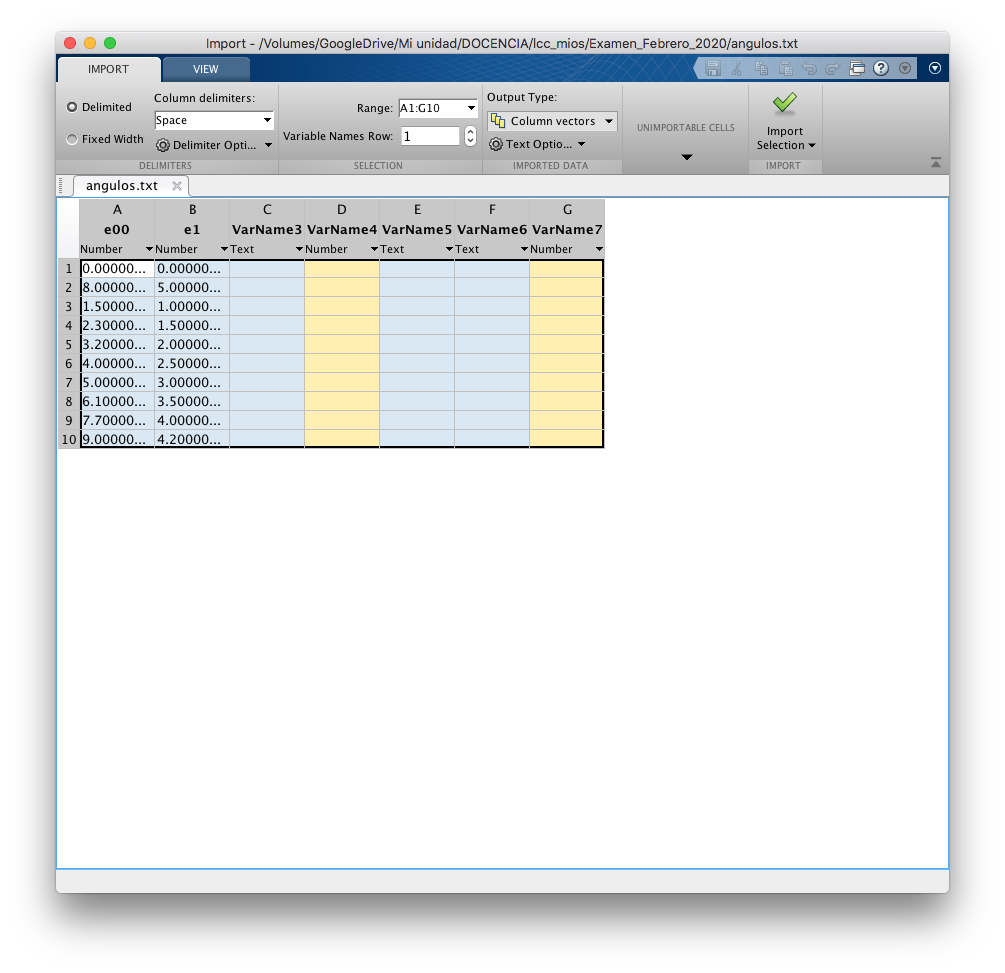
\includegraphics[width=10cm]{Wizard1.png}
	\caption{Aspecto de la herramienta de importación de datos}
	\label{fig:wizard}
\end{figure}

Para abrir en Matlab la herramienta de importación, basta pulsar en la pestaña \emph{home}, situada en la parte superior del IDE de Matlab,   el botón \emph{Import Data}. Matlab abre entonces una ventana que nos permite navegar por el árbol de directorio y seleccionar el archivo del que deseamos importar los datos. Una vez seleccionado, Matlab abre la ventana mostrada en la imagen \ref{fig:wizard}. 
Se trata de un programa especial ---\emph{import wizard}--- que sirve para guiar al usuario en el proceso de cargar las variables contenidas en el fichero en el \emph{workspace} de Matlab.


\newpage
\section{Ejercicios}
\begin{enumerate}
\item Tipos de variables en Matlab; matrices y vectores. Escribe, por orden, las siguientes expresiones en la \emph{línea de comandos} de Matlab e interpreta los resultados que obtienes. En los casos en que Matlab devuelva un mensaje de error, trata de averiguar la razón. \textbf{Nota:} Es importante hacerlos por orden ya que algunos operaciones se apoyan en los resultados de operaciones anteriores.
\begin{multicols}{2}
\begin{enumerate}
\renewcommand{\labelenumii}{\arabic{enumii}}
\texttt{
\item a=[1 2 3; 4 5 6]
\item a=[1 2 3; 4 5]
\item a=[ 1 2 3\\
1 2 3\\
1 2]
\item[*] Operador (:) para crear vectores
\item a=[1:10:0]
\item a=1:10:2
\item a=1:0.05:2
\item a=1:-0.05:-1
\item a=[1:10;2:12;3:13]
\item a=[1:10;2:11;3:12]
\item a=[1 2 7\\
5 6 8\\
3 2 6]
\item b=[1 2 3]
\item c=[a b]
\item c=[a;b]
\item d=[b;a]
\item[*] Operador (:) para indexar
\item c=[a(1,:) b]
\item c=[a(1:2,:);b]
\item c=[a(1:2,:);b;a(size(a,1),:)]
\item[*] Funciones para manipulación de matrices
\item a=[1 2 3]
\item b=diag(a)
\item c=diag(b)
\item M=size(c)
\item \ [m,n]=size(c)
\item m=size(c)
\item m=size(c,1)
\item m=size(c,2)
\item d=ones(size(a))
\item d=ones(size(b))
\item  d=ones(size(b,1))
\item d=ones(size(b,1),size(c,2))
\item f=eye(size(d,1))
\item who
\item whos
\item clear all
\item who
\item q=[1 2 3\\
4 5 6\\
7 8 9]
\item  r=diag(q,1)
\item  r=diag(q,2)
\item  r=diag(q,0)
\item  r=diag(q,-1)
\item  r=diag(q,-2)
\item  tt=eye(1,3)
\item  tt=eye(3,1)
\item  tt=eye(3)
\item  tt=eye(5)
\item  tt=eye(5,3)\\
\item  tt=eye(3,5)\\
\item a=[1 3 4\\
2 4 6]\\
\item  b=[2 3\\
4 5\\
6 7]
\item[*] Operadores aplicados a matrices
\item c=a*b
\item d=b*a
\item e=[ 1 2\\
4 5]
\item a*e
\item g=a*e
\item g=e*a
\item a*b
\item a=[1 3 4\\
5 6 8]
\item b=3
\item a*b
\item a.*b
\item b=[2 3]
\item a.*b
\item b=[ 2 3 4\\
5 6 7]
\item a.*b
\item c=b'
\item d=a'
\item r=a-b
\item h=a-a'
\item j=a+b
\item j=a'+b
\item d=(a+b)*b'
\item f=(a+b)*b'
\item f=(a-b)'*b
\item a=[ 1 3 5\\
2 5 6
3 4 2]
\item p=a\^{}2
\item r=a\^{}2-a*a
\item r=a.\^{}2-a*a
\item r=a\^{}2-a.*a
\item b=[ 3 5 6\\
2 1 1\\
1 2 3]
\item[*] Encadenando operaciones
\item w=a*b\^{}(-1)
\item w=a*inv(b)
\item w=a/b
\item w= a*b\^{}(-1)-a*inv(b)
\item w= a*b\^{}(-1)-a/b
\item w=a\^{}(-1)*b
\item w=inv(a)*b
\item w=a\textbackslash b
\item w= a\^{}(-1)*b-inv(a)*b
\item w=a\textbackslash b-inv(a)*b
\item w=a./b
\item w=a.\textbackslash b
\item w=a.\^{}(-1)*b
\item w=a.\^{}(-1)*b-a.\textbackslash b
}
\end{enumerate}
\end{multicols}
\item Obtén empleando la \emph{línea de comandos} de matlab el resultado de las siguientes expresiones:
\begin{multicols}{2}
\begin{align*}
\frac{5+3x^2}{6y}\\
\frac{1+4\sqrt{2x}}{6}y \\
\frac{-x+\sqrt{x^2-4xy}}{2x}
\end{align*}

\begin{align*}
\frac{1}{\sqrt{2\pi}}e^{-\frac{1}{2}(x-1)^2}\\
\sin^2(2x)+\cos^2(2x) \\
\arctan(\infty)\\
\arctan\left(\frac{y}{x}\right)
\end{align*}
\end{multicols}
Emplea para $x$ e $y$ tanto valores escalares como matrices.

\item Abre un fichero nuevo en el editor de textos de matlab.
Escribe las siguiente líneas:\\
\texttt{
x = A*B\\
y = A+B\\
z = A*sin(B)}\\
Guarda el fichero. Emplea el comando \verb|clear| all para limpiar el \emph{workspace}
Invoca el fichero desde matlab. ¿Qué sucede?\\
Crea en la ventana de comandos las matrices,
\begin{equation*}
A =\begin{pmatrix}
1&3&4\\
2&5&6\\
7&8&9
\end{pmatrix}, \ B=\begin{pmatrix}
2&6&8\\
3&7&8\\
2&7&9
\end{pmatrix}
\end{equation*}
Vuelve a ejecutar el programa guardado en el fichero.\\
Añade al programa, al principio del todo, la línea \texttt{clear all}. Guarda y vuelve a ejecutar el
programa. ¿Qué sucede ahora?\\
Introduce las matrices A y B directamente en el código del programa debajo de la línea \texttt{clear all}. Analiza qué sucede al ejecutar de nuevo el programa.\\
 Eliminar la línea \texttt{clear all}. Introduce a través de la ventana de comando dos matrices $A$ y $B$ distintas de las que contiene el programa. Ejecuta el programa y comprueba qué matrices utiliza para realizar los cálculos.\\
Comenta la(s) línea(s) de código donde has definido las matrices $A$ y $B$ en el programa. Añade al principio del programa una línea para convertir el script en una función:\\
\verb|function [x] = nombre_de_tu_programa(A,B)| \\
Invoca la función recién creada desde la \emph{línea de comandos} de matlab. Observa lo que pasa si la invocas como:
\begin{verbatim}
>>nombre_de_tu_programa
>>nombre_de_tu_programa(F)
>>nombre_de_tu_programa(F,J)
\end{verbatim}
Introduce, en el  workspace de matlab --usando la \emph{línea de comandos}--  las matrices $F$ y $J$, dondo,
\begin{equation*}
F =\begin{pmatrix}
1&0&1\\
2&0&4\\
3&5&0
\end{pmatrix}, \ J=\begin{pmatrix}
1&6&7\\
2&9&0\\
4&4&4
\end{pmatrix}
\end{equation*}
Vuelve a ejecutar, \verb|>>nombre_de_tu_programa(F,J)| \\
Genera dos matrices de tamaño $(3\times 3)$. Nómbralas como prefieras: \verb|mi_matriz1, mi_matriz2|. Ejecuta ahora,
\begin{verbatim}
>>nombre_de_tu_programa(mi_matriz1,J)
>>nombre_de_tu_programa(mi_matriz2,F)
>>nombre_de_tu_programa(mi_matriz1,mi_matriz2)
>>resultado=nombre_de_tu_programa(F,J)
>>[r1,r2]=nombre_de_tu_programa(F,J)
>>[A,B;r3]=nombre_de_tu_programa(F,J)
>>[A,B;C]=nombre_de_tu_programa(A,B)
\end{verbatim}
Crea un nuevo fichero, con el siguiente código:
% \begin{lstlisting}
% A=sin(B).*cos(C)
% [D,E,F]=nombre_de_tu_programa(A,C)
% G = D + E - F
% \end{lstlisting}
Guárdalo con el nombre que quieras.\\
Define en la \emph{línea de comandos} matrices $B$ y $C$ adecuadas para el programa que acabas de escribir y ejecútalo.\\
Añade al programa una primera línea de código que lo convierta en una función que tome como entradas las matrices $B$ y $C$  y que:\\
devuelva solo la matriz $G$\\
devuelva las matrices $G$ y $D$\\ 
devuelva las matrices $G$,$D$,$E$ y $F$.

Escribe una nueva función con el siguiente código,
\begin{minted}[
frame=lines,
framesep=2mm,
baselinestretch=1.2,
%bgcolor=LightGray,
fontsize=\footnotesize,
linenos
]{python}
import numpy as np
def nombre_de_la_funcion(B,C):
    E= B + C**2
    D =B - C.inv()
    return(E,D)
% A=nombre_funcion_dentro(E,D);
% end;
% function s=nombre_funcion_dentro(l,p);
% s=l + p - 2;
% end;
\end{minted}

Crea matrices $B$ y $C$ adecuadas y ejecuta la función que acabas de crear. Describe cómo funciona.

\item Define en la \emph{línea de comandos} las matriz $M$ y $N$ e interpreta el resultado de las condiciones lógicas impuestas.

\begin{equation*}
M =\begin{pmatrix}
1&2&3\\
4&5&6\\
7&8&9
\end{pmatrix}, \ N=\begin{pmatrix}
2&3&4\\
5&6&7\\
8&9&10
\end{pmatrix}
\end{equation*}
\begin{verbatim}
>>y=m<2
>>y=m<=2
>>y=m>2
>>y=m>=2
>>y=m==2
>>y=m~=2
>>y=any(m<2)
>>y=any(m<2,1)
>>y=any(m<2,2)
>>y=any(m==2)
>>y=all(m>=2)
>>y=all(m~=0)
>>y=all(any(m<2))
>>y=any(all(m<2))

>> index=find(m>2)
>>[i,j]=find(m<5)

>> y=any(m<2)&any(n>4)
>> y=any(m<2)&any(n>10)
>> y=any(m<2)&any(n>6)
>> y=any(m<2)&any(n>7)
>> y=any(m<2)&any(n>3)
>> y=any(m<2)&any(n>2)
>> y=any(m>2)&any(n>2)
>> y=any(m>4)&any(n>2)
>> y=any(m>4,1)&any(n>2)
>> y=any(m>4,2)'&any(n>2)
\end{verbatim}
Repite el estudio de las condiciones lógicas cambiando \& por \textbar

\item Escribe el siguiente código en un fichero. Ejecútalo y analiza los resultados,
% \begin{lstlisting}
% dato=rand(1)
% if dato==0.5
%  dato=0
% elseif dato<0.5
%  dato=-dato*10
% else
%  dato=dato*10
% end
% \end{lstlisting}

Modifica el programa,
\begin{enumerate}
\item Para que no muestre los resultados de los cálculos por pantalla
\item para que, utilizando comandos \verb|elseif, &| devuelva una variable (distinta de 'dato') con valor $-1$ si se cumple que 'dato' es menor o igual que $0.3$, con valor $-0.5$ si 'dato' es mayor que $0.3$ y menor que $0.5$, con valor $0$ si 'dato' es mayor o igual que $0.5$ y menor  o igual que $0.7$ y con valor $1$ en cualquier otro caso.
\item Convierte el \emph{script}, en una función, que tome 'dato' como variable de entrada, y devuelva el valor de la variable obtenida, según la condición que se cumpla. (Lógicamente se debe eliminar o comentar la línea \verb|dato=rand(1)|).
\end{enumerate}

\item Crea un scrip de matlab con el siguiente código y trata de adivinar qué hace antes de ejecutarlo. Utiliza el \emph{help} de matlab para averiguar lo que hace la función \verb|abs|.
% \begin{lstlisting}
% n=10
% for i=1:n
%  for j=1:n
%   if i==j
%    a(i,j)=1;
%   elseif abs(i-j)==1
%    a(i,j)=-1
%   else
%    a(i,j)=0
%   end
%  end
% end
% \end{lstlisting}

Introduce un punto de ruptura (\emph{breakpoint}) en el código, por ejemplo en la línea 12. Ejecuta paso a paso el programa para ver como va generando el resultado. Intercambia los índices \verb|i,j| de la matriz \verb|a|. \verb|a(j,i)|.¿Se obtiene el mismo resultado? ¿Cómo se construye ahora la matriz?

\item Crea un script con el siguiente código,
\begin{minted}[
frame=lines,
framesep=2mm,
baselinestretch=1.2,
%bgcolor=LightGray,
fontsize=\footnotesize,
linenos
]{python}
i=0
while i<10:
    i=i+1
    j=0
    while j<10:
        j=j+1
        if i==j:
            a[i,j+=1;
        elif abs(i-j)==1:
            a[i,j]=-1
        else:
            a(i,j)=0
\end{minted}

Repite el estudio del programa anterior

\item Modifica el \emph{script} anterior de modo que quede el siguiente código,
% \begin{lstlisting}
% i=0
% while(1)
%  i=i+1
%  j=0
%  while(1)
%   j=j+1
%   if i==j
%    a(i,j)=1;
%   elseif abs(i-j)==1
%    a(i,j)=-1
%   else
%    a(i,j)=0
%   end
%   if j==10
%    break
%   end
%  end
%  if i==10
%   break
%  end
% end
% \end{lstlisting}
Repite el estudio del programa anterior. ¿Qué sucede si comentamos la(s) línea(s) que contiene la sentencia \verb|break|?
Reconvierte los \emph{scrips} anteriores en funciones que admitan como variable de entrada el tamaño de la matriz que se desea generar y devuelvan como variable de salida la matriz creada.

\item Dada una matriz $A \in \mathbb{R}^{n\times n}$ y un vector columna $v \in \mathbb{R}^n-{\mathbf{0}}$. Se dice que el vector $v$ pertenece al \emph{Kernel} de $A$ si se cumple que $Av =\mathbf{0}$.



Crea una función que tome como variables de entrada una matriz $A$ cuadrada de cualquier dimension $n\times n$ y un vector columna de dimensión $n$ y compruebe si$n$ pertenece o no al \emph{kernel} de $A$. \textbf{Nota:} Considera que la condición se cumple si todos los elementos del vector $Av$ son menores que $1e-12$.

\item Escribe ---empleando bucles y sin hacer uso del operador ( \^\ ) --- una función \verb|potencia.m| que reciba como argumentos de entrada un número real $x\in \mathbb{R}$ y un entero $n \in \mathbb{Z}$ y devuelva el valor de la n-ésima potencia de $x$ ($x^n$). El segundo argumento de entrada puede ser opcional. Si se omite debe tomarse como $n=2$ (devolviendo el cuadrado de $x$). Ver la función interna nargin. \textbf{Nota:} Ten en cuenta que $n$ puede ser positivo, negativo o cero.

\item Crea una función que determine la suma de los inversos de los números naturales impares menores de 1000. Usa las funciones tic y toc para determinar el tiempo que se tarda. Emplea bucles para el cálculo.
\begin{equation*}
S_{imp} = \sum_{n=1}^{500}\frac{1}{2n-1} =\frac{1}{1}+\frac{1}{3}+\frac{1}{5}+\cdots+\frac{1}{999}
\end{equation*}
Modifica tu programa, de modo que admita como variable de entrada un número $m\in\mathbb{N}$ y calcule el valor de la suma de los inversos de los impares menores o iguales que $m$.

\item Los números de Fibonacci, $F(n)$ son una serie de números naturales. Los dos primeros valores de la serie son:  $F(1)=1$ y $F(2)=2$. Los demás términos se calculan como la suma de los dos anteriores: $F(n) = F(n-1) + F(n-2)$.
Escribe un script que genere los primeros $m$ números de la serie de Fibonacci, almacenándolos en un vector \verb|F|. Emplea para el cálculo la estructura \verb|while|.

\item Sin utilizar las funciones de matlab \verb|flip,fliplr, flipud,...|, escribe las líneas de código para que, dado un vector \verb|x|, genere otro vector con el orden de los elementos invertido.
\end{enumerate}

\section{Test del curso 2020/21}
\begin{enumerate}

\item  El movimiento de un cuerpo en el plano viene descrito por las siguientes ecuaciones,

\begin{align}
x(t) &= \sin(2 \pi \, \omega_1 t)\\
y(t) &= \cos(2 \pi \, \omega_2 t)\\
z(t) &= a\cos(2\pi \, \omega_1 t) \label{eq:3}
\end{align}

donde $x,y,z$ representan las coordenadas del cuerpo en el instante de tiempo $t$ medidas en metros,  $w_1$ y $w_2$ son frecuencias fijas medidas en $rad\cdot s^{-1}$ y $a$ es una amplitud fija medida en metros.

\begin{enumerate}
	\item \label{ap1} (\textbf{1.5 puntos}) Escribe una función que:

\begin{enumerate}
	\item Tome como variables de entrada las frecuencias $w_1$, $w_2$, la amplitud $a$ .
	\item Haga el cálculo de la trayectoria en tres dimensiones descrita por el cuerpo en el intervalo de tiempo $[0,1]$. Considera incrementos de tiempo de $0.01s$.
	\item Dibuje en una gráfica la trayectoria descrita por el cuerpo en el espacio. Cada eje del gráfico deberá llevar  una etiqueta indicando de qué variable se trata $x$, $y$ ó $z$.
	\item La salida serán tres vectores con los valores de $x$, $y$ y $z$ calculados para cada instante de tiempo.
	\end{enumerate}

\item (\textbf{1.5 puntos}) Añade a la función creada en el apartado anterior el código necesario para que:
	\begin{enumerate}
	\item \textbf{Solo si} se le dan dos variables de entrada en lugar de tres, entonces calcule la trayectoria que describiría el cuerpo en el plano si se eliminara la ecuación (\ref{eq:3}) de las ecuaciones del sistema. (NOTA: La función debe seguir funcionando igual que en el apartado anterior si se le dan tres entradas. Emplea el comando nargin).
	\item El resultado deberá también representarse gráficamente, pero solo en dos dimensiones, y devolver la variable $z$ como un vector vacío. 
	\end{enumerate}

\item \label{ap2} (\textbf{1.5 puntos}) Crea un un \emph{live script} que genere dos  vectores de frecuencias: \texttt{W1} y \texttt{W2} de  modo que el primero contenga los números impares comprendidos entre $1$ y $7$ y el segundo los números pares comprendidos entres $2$ y $8$.  Emplea la función creada en el apartado anterior para calcular el valor de las trayectorias obtenidas tomando como entradas para  $\omega_1, \omega_2$,  todos los pares posibles de la forma: \texttt{W1(i)} y \texttt{W2(j)}. Supón que no hay tercera entrada $a$. Realiza los cálculos empleando bucles.

\item (\textbf{1 punto}) Añade a tu programa el código necesario para que dibuje cada resultado en un \emph{subplot} de modo que la figura resultante tenga $4\times4$ \emph{subplots} (ver figura al dorso).  Debes crear los \emph{subplots} empleando los mismos bucles del apartados anterior. 

\item (\textbf{0.5 puntos}) Repite los cálculos de los apartados c) y d) pero tomando ahora $a=1$.
\end{enumerate}

\item Una matriz cuadrada $A$, de dimensión arbitraria $(n\times n)$, cuyos elementos $a_{ij} \in \mathbb{Z}$, se define como \emph{buenrollista} cuando las suma de los valores pares de cada fila es mayor o igual que la suma de los valores  impares de la columna correspondiente, i.e., satisface la siguiente relación:
\begin{equation}
	\sum_{j=1}^n a_{ij\text{(par)}} \geq \sum_{j=1}^n a_{ji\text{(impar)}}, \quad \forall i\in\{1,...,n\}
\end{equation}

\begin{enumerate}
\item (\textbf{1.5 puntos}) Escribe  una función que tome como variable de entrada una matriz cuadrada de cualquier dimensión 
y calcule un vector con las sumas de los valores pares de los elementos de cada una de su filas  y otro vector con las sumas de los elementos impares de cada una de sus columnas.
\item (\textbf{1.5 puntos}) Añade a la función anterior el código necesario para que compruebe, empleando los vectores obtenidos en el apartado anterior, si la función es \emph{buenrollista} y muestre un mensaje por pantalla indicando si lo es o no.
\item (\textbf{1 punto}) Aplica la función desarrollada a la siguiente matriz:
\begin{equation*}
\begin{pmatrix}
2&3&4&6&1\\
5&4&-2&3&0\\
4&-1&5&4&-6\\
4&2&4&5&8\\
3&0&-3&-3&6
\end{pmatrix}
\end{equation*}
\end{enumerate}
\end{enumerate}
\noindent\rule{\textwidth}{0.4pt}
\begin{figure}[h]
\centering
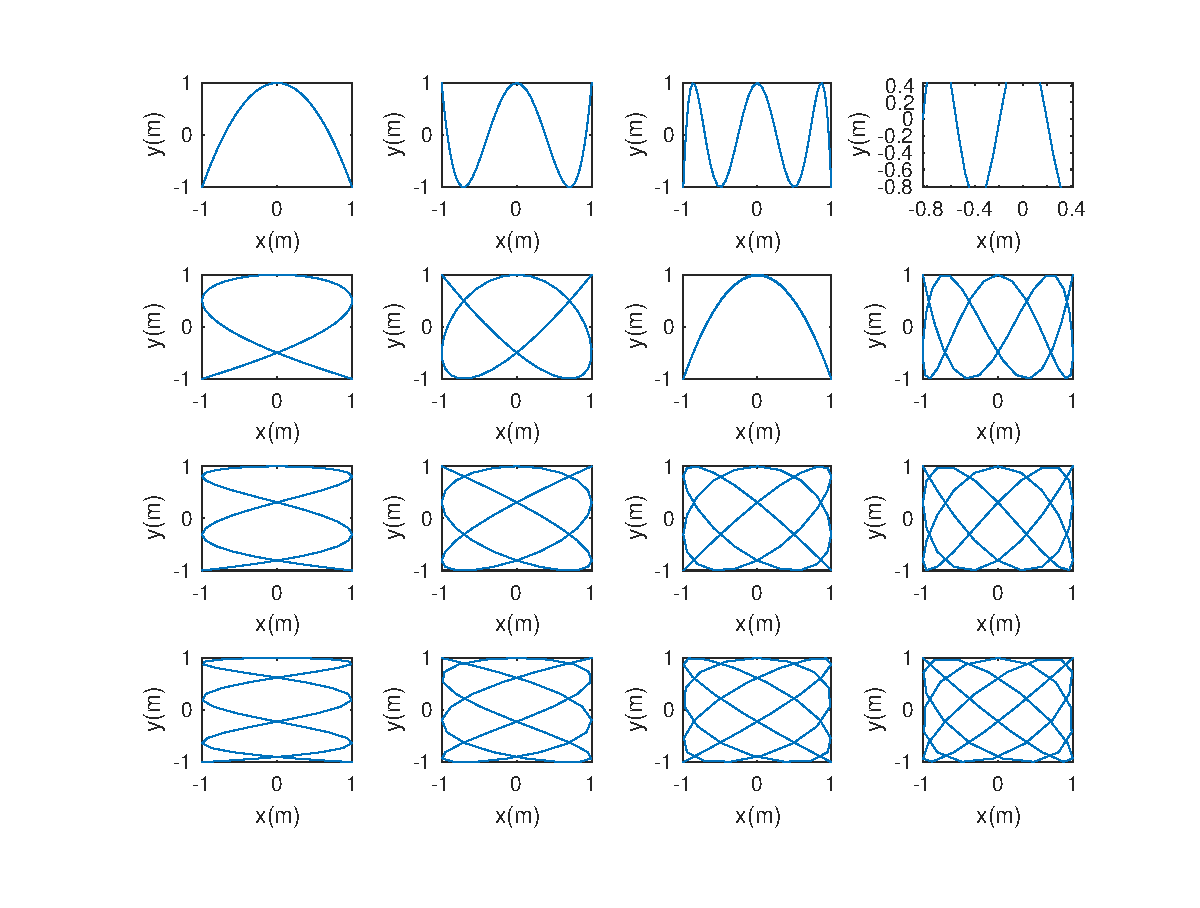
\includegraphics[scale=0.5]{lisa1.eps}
\caption{vista de la figura con los ocho subplots} \label{fig:1}
\end{figure}
